\documentclass[a4paper,12pt,twoside]{report}
\usepackage[utf8]{inputenc}
\usepackage[T1]{fontenc}
%\usepackage{times}
\usepackage[margin=3cm,left=2cm,right=1.5cm]{geometry}
%\usepackage[a4paper]{geometry}
\usepackage[brazilian]{babel} %french
\usepackage{colortbl}
\usepackage{fancyhdr}
\usepackage{lastpage}
\usepackage{multicol}
\usepackage{multirow}
\usepackage{array}
\usepackage{booktabs}
\usepackage{pdfpages}
\usepackage{subcaption}
\usepackage[hyperindex=true]{hyperref}
\usepackage{xspace}
\usepackage{qsymbols}
\usepackage{soul}
\usepackage[portuges]{varioref}
\usepackage{tabulary}
\usepackage{tabularx}
\usepackage{framed}
\usepackage{amsmath}
\usepackage{graphicx}
\usepackage{listings}
\usepackage[long,dayofweek]{datetime}
\usepackage{todonotes}
%\usepackage[disable]{todonotes}
\usepackage{titlesec}

\graphicspath{{.}{figs/}}

\hypersetup
{
  bookmarksopen=true,
  pdftitle="Notas de aula - Pesquisa e Ordenação de Dados A",
  pdfauthor="Joao Vicente Ferreira Lima", 
  pdfsubject="notas de aula", 
  pdftoolbar=false, 
  pdfmenubar=true,
  pdfhighlight=/O,
  pdfpagemode=UseNone,
  pdfpagelayout=SinglePage,
  pdffitwindow=true,
%  colorlinks=false,
  colorlinks=true,
%  linkcolor=linkcol,
%  citecolor=citecol,
%  urlcolor=linkcol
}

\titleformat{\chapter}{\normalfont\LARGE\bfseries}{\thechapter}{1em}{}
\titlespacing*{\chapter}{0pt}{3.5ex plus 1ex minus .2ex}{2.3ex plus .2ex}

\lstset{%
	language=C,
	basicstyle=\small\ttfamily,
	keywordstyle=\bfseries,
	commentstyle=\itshape,
%	commentstyle=\slshape\color{green!50!black},
%	keywordstyle=\bfseries\color{blue!50!black},
%	stringstyle=\color{red},
	numbers=left,
	escapechar=\#,
%	emphstyle=\bfseries\color{red}
}

\newtheorem{theorem}{Teorema}

\renewcommand{\headrulewidth}{0pt}
\renewcommand{\footrulewidth}{0pt}
\fancyhf{}
\fancypagestyle{plain}{
  \fancyhead{}
  \fancyfoot{}
  \renewcommand{\headrulewidth}{0pt}
  \renewcommand{\footrulewidth}{0pt}
}
%\fancyfoot[C]{\footnotesize Pesquisa e Ordenação de Dados ``A''~--~UFSM \hfill \thepage}
\fancyhead[LE]{\slshape\footnotesize \leftmark}
\fancyhead[RO]{\slshape\footnotesize \rightmark}
\fancyfoot[C]{\footnotesize\thepage}



\title{{\bf Notas de aula\\
Pesquisa e Ordenação de Dados ``A''}}

\author{
João Vicente Ferreira Lima\\
Departamento de Linguagens e Sistemas de Computação\\
Universidade Federal de Santa Maria
}

\date{\today}

\begin{document}
\maketitle

Versão compilada em \today.
Esta obra está licenciada sob uma licença \href{http://creativecommons.org/licenses/by-nc-nd/4.0/deed.pt_BR}{Creative Commons} (Atribuição-NãoComercial-SemDerivações 4.0 Internacional).

Material baseado nas aulas do prof. Sérgio Luis Sardi Mergen (UFSM) e slides do
livro ``Projeto de Algoritmos'' do prof. Nivio Ziviani.

\pagestyle{fancy}

\setcounter{tocdepth}{3}
\setcounter{secnumdepth}{3}
\tableofcontents

%%%%%%%%%%%%%%%%%%%%%%%%%%%%%%%%%%%%%%%%%%%%%%%%%%%%%%%%%%%%%%%%%%%%%%%%%%%%%%%
\chapter{Introdução}
%%%%%%%%%%%%%%%%%%%%%%%%%%%%%%%%%%%%%%%%%%%%%%%%%%%%%%%%%%%%%%%%%%%%%%%%%%%%%%%

As mídias de armazenamento podem ser analisadas por diversos aspectos como:
\begin{itemize}
\item velocidade de acesso aos dados.
\item custo unitário.
\item confiabilidade nos casos de perda de dados por desligamento de energia
ou falha no sistema, ou ainda falha física.
\end{itemize}

As mídias podem ser classificadas de duas formas:
\begin{itemize}
\item {\bf Armazenamento volátil} - perde o conteúdo quando a energia é desligada.
Ex.: memória principal (RAM).
\item {\bf Armazenamento não volátil} - o conteúdo permanece (persiste) mesmo após
o desligamento da energia.
Ex.: memórias secundários (como disco rígido) e terceária.
\end{itemize}

%%%%%%%%%%%%%%%%%%%%%%%%%%%%%%%%%%%%%%%%%%%%%%%%%%%%%%%%%%%%%%%%%%%%%%%%%%%%%%%
\section{Memória principal}
%%%%%%%%%%%%%%%%%%%%%%%%%%%%%%%%%%%%%%%%%%%%%%%%%%%%%%%%%%%%%%%%%%%%%%%%%%%%%%%

\todo[inline]{Texto.}

%%%%%%%%%%%%%%%%%%%%%%%%%%%%%%%%%%%%%%%%%%%%%%%%%%%%%%%%%%%%%%%%%%%%%%%%%%%%%%%
\section{Memória secundário}
%%%%%%%%%%%%%%%%%%%%%%%%%%%%%%%%%%%%%%%%%%%%%%%%%%%%%%%%%%%%%%%%%%%%%%%%%%%%%%%

\todo[inline]{Texto.}
%%%%%%%%%%%%%%%%%%%%%%%%%%%%%%%%%%%%%%%%%%%%%%%%%%%%%%%%%%%%%%%%%%%%%%%%%%%%%%%
\section{Memória terciária}
%%%%%%%%%%%%%%%%%%%%%%%%%%%%%%%%%%%%%%%%%%%%%%%%%%%%%%%%%%%%%%%%%%%%%%%%%%%%%%%

\todo[inline]{Texto.}

%%%%%%%%%%%%%%%%%%%%%%%%%%%%%%%%%%%%%%%%%%%%%%%%%%%%%%%%%%%%%%%%%%%%%%%%%%%%%%%
\section{Aula 02}
%%%%%%%%%%%%%%%%%%%%%%%%%%%%%%%%%%%%%%%%%%%%%%%%%%%%%%%%%%%%%%%%%%%%%%%%%%%%%%%

%%%%%%%%%%%%%%%%%%%%%%%%%%%%%%%%%%%%%%%%%%%%%%%%%%%%%%%%%%%%%%%%%%%%%%%%%%%%%%%
\subsection{Definição de algoritmo}

\begin{itemize}
\item Procedimento bem definido que:
	\begin{itemize}
	\item recebe como entrada um valor, ou conjunto de valores
	\item produz como saída um valor ou conjunto de valores
	\end{itemize}
\item Conjunto de passos que transforma a entrada na saída.
\item Exemplo do {\bf problema de ordenação}:
\end{itemize}

{\bf Entrada}: uma sequência de $n$ números $\langle a_1, a_2, ..., a_n \rangle$.

{\bf Saída}:  Uma permutação $\langle {a'}_1, {a'}_2, ..., {a'}_n \rangle$ da
entrada tal que ${a'}_1 \leq {a'}_2 \leq ... \leq {a'}_n \rangle$.

\begin{itemize}
\item Essa entrada do algoritmo é uma {\bf instância} do problema.
\item Para um algoritmo estar {\bf correto}, para cada instância, ele termina com saída 
correta. Um algoritmo correto \textsf{resolve} um problema. 
\end{itemize}

Exemplos de problemas:
\begin{itemize}
\item O Projeto do Genoma Humano para identificar todos os genes do DNA humano.
\item Internet com descoberta de rotas.
\item E-commerce.
\end{itemize}

%%%%%%%%%%%%%%%%%%%%%%%%%%%%%%%%%%%%%%%%%%%%%%%%%%%%%%%%%%%%%%%%%%%%%%%%%%%%%%%
\subsection{Análise de algoritmos}

Pergunta fund


\part{Classificação de dados}
%%%%%%%%%%%%%%%%%%%%%%%%%%%%%%%%%%%%%%%%%%%%%%%%%%%%%%%%%%%%%%%%%%%%%%%%%%%%%%%
\chapter{Classificação de dados}
%%%%%%%%%%%%%%%%%%%%%%%%%%%%%%%%%%%%%%%%%%%%%%%%%%%%%%%%%%%%%%%%%%%%%%%%%%%%%%%

Os algoritmos deste capítulo resolvem o {\bf problema de ordenação}:
\begin{itemize}
\item {\bf Entrada}: uma sequência de $n$ números $\langle a_1, a_2, ..., a_n \rangle$.

\item {\bf Saída}:  Uma permutação $\langle {a'}_1, {a'}_2, ..., {a'}_n \rangle$ da
entrada tal que ${a'}_1 \leq {a'}_2 \leq ... \leq {a'}_n$.
\end{itemize}
Ordenação pode ser usado em diversos outros algoritmos.
Ela pode ser necessária devido a requisitos do usuário, ou para a otimização de pesquisa 
como na pesquisa binária.

Em geral os dados são mantidos em um vetor onde cada objeto possui um
atributo \textbf{chave} que deve ser mantido ordenado.
Para fins de exemplo, utiliza-se números inteiros como elementos.

Um algoritmo de ordenação possui duas características principais:
\begin{itemize}
\item {\bf Estabilidade} -- relativo a manutenção da ordem original dos itens 
com chaves iguais.
	\begin{itemize}
	\item Um algoritmo de ordenação é {\bf estável} se a ordem relativa dos itens
		com chaves iguais não se altera durante a ordenação.
	\end{itemize}
\item {\bf Uso de memória} -- quanto ao uso de memória pelo algoritmo.
	\begin{itemize}
	\item {\bf Com cópia de dados} -- utiliza um vetor temporário para realizar a ordenação. As trocas são feitas entre o vetor original e o temporário.
	\item {\bf In-place} -- as trocas são feitas dentro do próprio vetor original.
	\end{itemize}
\end{itemize}

O critério de avaliação, sendo $n$ o número de registros, pode ser por:
\begin{itemize}
\item $C(n)$ -- número de comparações.
\item $M(n)$ -- número de movimentações de elementos.
\end{itemize}
Em grande parte dos casos, nos concentramos no número de comparações.

Os métodos de ordenação podem ser {\bf interno} (em memória primária) ou {\bf externo} (em memória secundária).
Na {\bf interna} o arquivo de entrada cabe todo na memória principal, enquanto
que na {\bf externa} o arquivo não cabe na memória principal. 

A maioria dos métodos é baseada em {\bf comparações} de chaves.
Porém, existem outros métodos que utilizam o principio da {\bf distribuição}. 
Um exemplo é ordenar um baralho com 52 cartas na ordem numérica e ordem de naipes.
O algoritmo seria:
\begin{enumerate}
\item Distribuir cartas em treze montes: ases, dois, três, ...., reis.
\item Coletar os montes na ordem especificada.
\item Distribuir novamente as cartas em quatro montes: paus, ouros, copas e espadas.
\item Coletar os montes na ordem especificada.
\end{enumerate}
Alguns desses métodos são o {\bf radixsort} e o {\bf bucketsort}.

%%%%%%%%%%%%%%%%%%%%%%%%%%%%%%%%%%%%%%%%%%%%%%%%%%%%%%%%%%%%%%%%%%%%%%%%%%%%%%%
\section{Classificação em memória primária}
%%%%%%%%%%%%%%%%%%%%%%%%%%%%%%%%%%%%%%%%%%%%%%%%%%%%%%%%%%%%%%%%%%%%%%%%%%%%%%%

Podem ser classificados como:
\begin{itemize}
\item {\bf Métodos simples} -- adequado para vetores pequenos, requerem $O(n^2)$ comparações.
Ex.: bolha, inserção, seleção, shellsort.
\item {\bf Métodos eficientes} -- adequados para vetores grandes, requerem $O(n \log n)$ comparações.
Ex.: quicksort, mergesort, heapsort.
\item {\bf Métodos mais eficientes} -- requerem $O(n)$ atribuições. Ex.: radixsort.
\end{itemize}

%%%%%%%%%%%%%%%%%%%%%%%%%%%%%%%%%%%%%%%%%%%%%%%%%%%%%%%%%%%%%%%%%%%%%%%%%%%%%%%
\subsection{Bolha (\emph{bubble sort})}

O algoritmo é ilustrado na figura~\ref{aula03:algo:bubblesort}.
\begin{figure}[!htb]
\centering
\begin{framed}
\begin{lstlisting}
void Bubblesort( int *A, int n ){
	int i;
	bool trocado;
	do{
		trocado = false;
		for( i = 1; i < n; i++){
			if( A[i-1] > A[i] ){
				troca( A[i-1], A[i] );
				trocado = true;
			}
		}
	} while(trocado);
}
\end{lstlisting}
\end{framed}
\caption{Algoritmo do bubblesort.}
\label{aula03:algo:bubblesort}
\end{figure}

O número de comparações é $(n-1)+(n-2)+....+2+1$ com complexidade (para qualquer caso)
\begin{equation*}
C(n) = \sum_{k=1}^{n-1} i = \frac{n(n-1)}{2} = O(n^2).
\end{equation*}

As principais vantagens:
\begin{itemize}
\item Algoritmo simples.
\item Algoritmo estável.
\end{itemize}
Desvantagens:
\begin{itemize}
\item Se o vetor estiver ordenado, não melhora o tempo pois continua quadrático.
\end{itemize}

%%%%%%%%%%%%%%%%%%%%%%%%%%%%%%%%%%%%%%%%%%%%%%%%%%%%%%%%%%%%%%%%%%%%%%%%%%%%%%%
\subsection{Seleção (\emph{selection sort})}

O algoritmo é ilustrado na figura~\ref{aula03:algo:selection}.
\begin{figure}[!htb]
\centering
\begin{framed}
\begin{lstlisting}
void Selecao( int *A, int n ){
	int i, j, min;
	for( i = 0; i < n; i++){
		min = i;
		for(j= i+1; j < n; j++)
			if( A[j] < A[min] )	min = j;
		troca( A[min], A[i] );
	}
}
\end{lstlisting}
\end{framed}
\caption{Algoritmo por seleção.}
\label{aula03:algo:selection}
\end{figure}

O número de comparações é $(n-1)+(n-2)+....+2+1$ com complexidade (qualquer caso)
\begin{equation*}
C(n) = \sum_{k=1}^{n-1} i = \frac{n(n-1)}{2} = O(n^2).
\end{equation*}

Vantagens:
\begin{itemize}
\item custo linear para movimentações.
\item interessante para vetores pequenos.
\end{itemize}
Desvantagens:
\begin{itemize}
\item vetor ordenado não ajuda, pois o custo continua quadrático.
\item algoritmo {\bf não é estável}.
\end{itemize}

%%%%%%%%%%%%%%%%%%%%%%%%%%%%%%%%%%%%%%%%%%%%%%%%%%%%%%%%%%%%%%%%%%%%%%%%%%%%%%%
\subsection{Inserção (\emph{insertion sort})}

A figura~\ref{aula02:algo:insertion} da seção~\ref{aula02:sec:insertion} ilustra
o algoritmo.
%
O número de comparações é $(n-1)+(n-2)+....+2+1$ no pior caso (ordem reversa), com complexidade
\begin{equation*}
C(n) = \sum_{k=1}^{n-1} i = \frac{n(n-1)}{2} = O(n^2).
\end{equation*}
Por outro lado, o número de comparações no melhor caso (vetor ordenado) é 
$1 + 1 + 1 + 1+ .... + 1 = n-1$ com complexidade
\begin{equation*}
C(n) = n - 1  = O(n).
\end{equation*}

Vantagens:
\begin{itemize}
\item ideal quando o vetor está ``quase'' ordenado.
\item ordenação estável.
\end{itemize}
Desvantagens:
\begin{itemize}
\item custo médio é quadratico.
\item alto custo para inserir elemento na posição correta.
\end{itemize}

%%%%%%%%%%%%%%%%%%%%%%%%%%%%%%%%%%%%%%%%%%%%%%%%%%%%%%%%%%%%%%%%%%%%%%%%%%%%%%%
\subsection{Shellsort}

%%%%%%%%%%%%%%%%%%%%%%%%%%%%%%%%%%%%%%%%%%%%%%%%%%%%%%%%%%%%%%%%%%%%%%%%%%%%%%%
\subsection{Comparação dos métodos básicos}

\begin{table}[!ht]
\centering
\begin{tabular}{lccccc}
\hline
          & Melhor caso & Caso médio & Pior caso & Memória & Estável \\ \hline
Bubble    & $O(n)$ & $O(n^2)$ & $O(n^2)$ & $1$ & sim \\ \hline
Selection & $O(n^2)$ & $O(n^2)$ & $O(n^2)$ & $1$ & não  \\ \hline
Insertion & $O(n)$ & $O(n^2)$ & $O(n^2)$ & $1$ &  sim \\ \hline
Shellsort & $O(n)$ & $O(n^{\frac{3}{2}})$ & $O(n^{\frac{3}{2}})$ &  $1$ & não \\ \hline
\end{tabular}
\end{table}

%%%%%%%%%%%%%%%%%%%%%%%%%%%%%%%%%%%%%%%%%%%%%%%%%%%%%%%%%%%%%%%%%%%%%%%%%%%%%%%
\subsection{Quicksort}

%%%%%%%%%%%%%%%%%%%%%%%%%%%%%%%%%%%%%%%%%%%%%%%%%%%%%%%%%%%%%%%%%%%%%%%%%%%%%%%
\subsection{Mergesort}

%%%%%%%%%%%%%%%%%%%%%%%%%%%%%%%%%%%%%%%%%%%%%%%%%%%%%%%%%%%%%%%%%%%%%%%%%%%%%%%
\subsection{Heapsort}

%%%%%%%%%%%%%%%%%%%%%%%%%%%%%%%%%%%%%%%%%%%%%%%%%%%%%%%%%%%%%%%%%%%%%%%%%%%%%%%
\subsection{Counting sort}

%%%%%%%%%%%%%%%%%%%%%%%%%%%%%%%%%%%%%%%%%%%%%%%%%%%%%%%%%%%%%%%%%%%%%%%%%%%%%%%
\subsection{Bucket sort}

%%%%%%%%%%%%%%%%%%%%%%%%%%%%%%%%%%%%%%%%%%%%%%%%%%%%%%%%%%%%%%%%%%%%%%%%%%%%%%%
\subsection{Radix sort}

%%%%%%%%%%%%%%%%%%%%%%%%%%%%%%%%%%%%%%%%%%%%%%%%%%%%%%%%%%%%%%%%%%%%%%%%%%%%%%%
\section{Classificação em memória secundária}
%%%%%%%%%%%%%%%%%%%%%%%%%%%%%%%%%%%%%%%%%%%%%%%%%%%%%%%%%%%%%%%%%%%%%%%%%%%%%%%

%%%%%%%%%%%%%%%%%%%%%%%%%%%%%%%%%%%%%%%%%%%%%%%%%%%%%%%%%%%%%%%%%%%%%%%%%%%%%%%
\section{Exercícios}
%%%%%%%%%%%%%%%%%%%%%%%%%%%%%%%%%%%%%%%%%%%%%%%%%%%%%%%%%%%%%%%%%%%%%%%%%%%%%%%


%%%%%%%%%%%%%%%%%%%%%%%%%%%%%%%%%%%%%%%%%%%%%%%%%%%%%%%%%%%%%%%%%%%%%%%%%%%%%%%
\chapter{Classificação em memória secundária}
%%%%%%%%%%%%%%%%%%%%%%%%%%%%%%%%%%%%%%%%%%%%%%%%%%%%%%%%%%%%%%%%%%%%%%%%%%%%%%%

Classificação em memória secundária, ou ordenação em memória externa, consiste
em ordenar arquivos de tamanho maior que a memória principal (interna)
disponível.
Nos algoritmos de ordenação externa deve-se reduzir o número de acessos ao disco,
resposável por grande parte do custo do algoritmo.

%Uma restrição que pode acontecer é o armazenamento de dados sequencial, como em
%fitas, discos e tambores magnéticos,.
%Ou também, quando somente um registro pode ser acessado em um dado momento.
%Esta última é uma restrições forte comparada ao acesso em vetores.

Os três principais fatores que diferenciam ordenação externa de interna são:
\begin{enumerate}
\item O custo para acessar um registro.
\item Restrições ao acesso físico, como em fitas magnéticas.
\item Tecnologia empregada.
\end{enumerate}

A maioria dos métodos de ordenação externa utiliza a seguinte estratégia:
\begin{enumerate}
\item Quebrar o arquivo em blocos do tamanho da memória interna disponível.
\item Ordenar cada bloco.
\item Intercalar os blocos ordenados, fazendo várias passadas.
\item A cada passada são criados blocos ordenados cada vez maiores, até que todo 
o arquivo esteja ordenado.
\end{enumerate}

Esses passos são agrupados em \textbf{passos}. 
O {\bf estágio de classificação} envolve os passos 1 e 2, enquanto que
o {\bf estágio de intercalação} consiste nos passos 3 e 4.
Os métodos para ordenação externa devem reduzir o número de passadas no arquivo.

Os conceitos usados neste capítulo são:
\begin{itemize}
\item {\bf Arquivo} - estrutura física de armazenamento. 
\item {\bf Partição} - estrutura lógica de armazenamento, que pode ser composto de
diversas partições.
\end{itemize}

%%%%%%%%%%%%%%%%%%%%%%%%%%%%%%%%%%%%%%%%%%%%%%%%%%%%%%%%%%%%%%%%%%%%%%%%%%%%%%%
\section{Classificação}
%%%%%%%%%%%%%%%%%%%%%%%%%%%%%%%%%%%%%%%%%%%%%%%%%%%%%%%%%%%%%%%%%%%%%%%%%%%%%%%

Considera-se que a memória principal tem capacidade para armazenar
$M$ registros do arquivo a classificar.

%%%%%%%%%%%%%%%%%%%%%%%%%%%%%%%%%%%%%%%%%%%%%%%%%%%%%%%%%%%%%%%%%%%%%%%%%%%%%%%
\subsection{Classificação interna}

A {\bf classificação interna} consiste na leitura de $M$  registros
para a memória, ordenação desses registros por qualquer outro algoritmo
de classificação interna e gravação desses registros classificados
em uma partição. 
Todas as partições ordenadas contêm $M$ registros, exceto (talvez) a última.

A {\bf classificação interna} envolve os seguintes passos:
\begin{enumerate}
\item leitura de $M$ registros para a memória.
\item ordenação desses registros por um algoritmo de ordenação interna.
	\begin{itemize}
	\item quicksort, mergesort, etc.
	\end{itemize}
\item gravação desses registros classificados.
	\begin{itemize}
	\item em uma partição nova de um arquivo existente (ou em novo arquivo).
	\end{itemize}
\end{enumerate}

A classificação interna possui a desvantagem de não explorar a ordem
parcial existente no arquivo de entrada.

%%%%%%%%%%%%%%%%%%%%%%%%%%%%%%%%%%%%%%%%%%%%%%%%%%%%%%%%%%%%%%%%%%%%%%%%%%%%%%%
\subsection{Seleção por substituição}

A {\bf seleção por substituição}  aproveita a possível classificação
parcial do arquivo de entrada. 
Em média, o tamanho das partições obtidas pelo processo de seleção com substituição
é de $2 * M$.

Os passos do algoritmo de seleção por substituição são:
\begin{enumerate}
\item Ler $M$ registros do arquivo para a memória.
\item Selecionar, na memória, o registro com menor chave.
\item Gravar na partição de saída o registro com menor chave.
\item Substituir (em memória) o registro gravado pelo próximo registro
do arquivo de entrada.
\item Caso a chave deste último seja menor do que a chave recém-gravada.
	\begin{enumerate}
	\item considerá-lo ``congelado'' e ignorá-lo no restante do processamento.
	\end{enumerate}
\item Caso existam em memória registros não ``congelados''
	\begin{enumerate}
	\item volta ao passo {\bf (2)}.
	\end{enumerate}
\item Caso contrário
	\begin{enumerate}
	\item fechar a partição de saída.
	\item ``descongelar'' os registros ``congelados''.
	\item abrir nova partição de saída.
	\item voltar ao passo {\bf (2)}.
	\end{enumerate}
\end{enumerate}

A seleção por substituição tem a desvantagem que no final da partição grande, 
parte do espaço em memória principal está ocupado com registros ``congelados''.

%%%%%%%%%%%%%%%%%%%%%%%%%%%%%%%%%%%%%%%%%%%%%%%%%%%%%%%%%%%%%%%%%%%%%%%%%%%%%%%
\subsection{Seleção natural}

A classificação por {\bf seleção natural} reserva um espaço na memória 
secundário (``\emph{o reservatório}''), que abriga os registros
``congelados'' em um processo de substituição.

A formação de uma partição se encerra quando o reservatório estiver cheio, ou
quando terminarem os registros de entrada.
Quando um reservatório encher, a memória é descarregada na partição atual
e os dados são copiados do repositório à memória.

A classificação por seleção natural usa como memória interna $M$ e um reservatório
que comporta $R$ registros.
Para $M = R$, o tamanho médio das partições é $M * e$ onde $e = 2,7182....$
(número de Euler).

Os passos do algoritmo de seleção natural são:
\begin{enumerate}
\item Ler $M$ registros do arquivo para a memória.
\item Selecionar, na memória, o registro com menor chave.
\item Gravar na partição de saída o registro com menor chave.
\item Substituir (em memória) o registro gravado pelo próximo registro
do arquivo de entrada.
\item Caso a chave deste último seja menor do que a chave recém-gravada.
	\begin{enumerate}
	\item gravá-lo no reservatório.
	\item substituir (em memória) o registro gravado no reservatório pelo
	próximo registro do arquivo de entrada.
	\end{enumerate}
\item Caso ainda exista espaço livre no reservatório.
	\begin{enumerate}
	\item volta ao passo {\bf (2)}.
	\end{enumerate}
\item Caso contrário
	\begin{enumerate}
	\item fechar a partição de saída.
	\item copiar os registros do reservatório para a memória.
	\item esvaziar o reservatório.
	\item abrir nova partição de saída.
	\item voltar ao passo {\bf (2)}.
	\end{enumerate}
\end{enumerate}

%%%%%%%%%%%%%%%%%%%%%%%%%%%%%%%%%%%%%%%%%%%%%%%%%%%%%%%%%%%%%%%%%%%%%%%%%%%%%%%
\subsection{Comparação de processos}

A classificação interna gera as menores partições, mas simplifica o estágio
de intercalação por usar partições de mesmo tamanho.
Os processos de seleção exigem intercalação mais elaborada, porém geram 
partições maiores, e reduzem o tempo de processamento.
A seleçõa natural gera as maiores partições, porém utiliza mais operações de 
entrada e saída. Além de usar memória externa adicional.

Os processos de seleção podem utilizar Heapsort para a ordenação interna.

%%%%%%%%%%%%%%%%%%%%%%%%%%%%%%%%%%%%%%%%%%%%%%%%%%%%%%%%%%%%%%%%%%%%%%%%%%%%%%%
\section{Intercalação}
%%%%%%%%%%%%%%%%%%%%%%%%%%%%%%%%%%%%%%%%%%%%%%%%%%%%%%%%%%%%%%%%%%%%%%%%%%%%%%%

O objetivo da intercalação é {\bf transformar um conjunto de partições classificadas em uma 
única partição classificada}.
Considera-se que a existência de $R$ partições geradas no particionamento.
O ideal seria intercalar todas as partições de uma só vez e obter o arquivo classificado.
Porém, todo sistema impõe um limite no número de arquivos abertos simultaneamente. 
Esse número pode ser menos que o número de partições geradas.

A intercalação exige uma série de passos, e em cada passo:
\begin{enumerate}
\item registros são lidos de um conjunto de partições dos arquivos de entrada.
\item e gravados em outro conjunto de partições de arquivos de saída.
\end{enumerate}

As operações de entrada e saída (E/S) tem um alto custo na ordenação externa.
Uma medida de eficiência do estágio de intercalação é dada pelo número de passos 
sobre os dados dado pela equação:
\begin{equation*}
N_{passos} = \frac{No. \; total \; de \; registros \; lidos}{No. \; total \;  de \; registros \; no \; arquivo \; classificado}
\end{equation*}
O menor número possível é $2$ ($1$ leitura e $1$ escrita).

%%%%%%%%%%%%%%%%%%%%%%%%%%%%%%%%%%%%%%%%%%%%%%%%%%%%%%%%%%%%%%%%%%%%%%%%%%%%%%%
\subsection{Intercalação balanceada de n caminhos}

A {\bf intercalação balanceada de n caminhos} usa $n$ arquivos para a entrada
de registros e outros $n$ arquivos para a saída de registros.  Sendo $F$ o
número máximo de arquivos que podem estar abertos ao mesmo tempo, $F = 2 n$.
Dessa forma, a intercalação balanceada de $n-$caminhos utiliza no máximo $F/2$
caminhos.

O particionamento inicial pode usar qualquer estratégia de particionamento.
{\bf Cada partição é escrita em um dos arquivos de entrada de forma intercalada}.

Os passos envolvidos são:
\begin{enumerate}
\item primeiro passo: determinar o número de arquivos ($F$) que o algoritmo irá
manipular, sendo a primeira metade ($F/2$) será usado para entrada enquanto
a outra metade ($F/2$) para saída.

\item passo dois: distribuir todas as partições, de forma {\bf intercalada},
nos arquivos de entrada.

\item {\bf passo de intercalação}: intercalar as primeiras partições,
gravando o resultado em um dos $F/2$ arquivos de saída, em ordem.

\item no final de cada fase, o conjunto de partições de saída
torna-se o conjunto de entrada.

\item a intercalação termina quando, em uma fase, grava-se apenas uma partição
(ordenada).
\end{enumerate}

%%%%%%%%%%%%%%%%%%%%%%%%%%%%%%%%%%%%%%%%%%%%%%%%%%%%%%%%%%%%%%%%%%%%%%%%%%%%%%%
\subsection{Intercalação ótima}

A {\bf intercalação ótima} usa $n$ arquivos para entrada e $1$ para saída
sendo $F = n + 1$.

O particionamento inicial pode usar qualquer estratégia de particionamento.
Ao contrário do particionamento na intercalação balanceada, {\bf o particionamento
inicial cria um novo arquivo por partição}.

Os passos envolvidos são:
\begin{enumerate}
\item primeiro passo: determinar o número de arquivos ($F$) que o algoritmo irá
manipular, sendo $F-1$ para entrada enquanto $1$ será de saída.

\item passo dois: abrir $F-1$ arquivos, cada um com uma partição. 

\item {\bf passo de intercalação}: intercalar as partições dos arquivos de entrada,
gravando o resultado em ordem no arquivo de saída.

\item o arquivo de saída é novo no primeiro passo, e é um dos arquivos já
inteiramente lidos nos próximos passos.

\item quando todas as partições ficarem vazias, os arquivos usados podem ser descartados.
O arquivo de saída vira um novo arquivo de entrada e é adicionado aos demais arquivos
de entrada não processados.

\item a intercalação termina quando restar apenas $1$ arquivo de entrada.
\end{enumerate}

O problema da intercalação ótima é que cada partição usa um arquivo próprio.
Esse número de arquivos pode ser grande.

%%%%%%%%%%%%%%%%%%%%%%%%%%%%%%%%%%%%%%%%%%%%%%%%%%%%%%%%%%%%%%%%%%%%%%%%%%%%%%%
\subsection{Intercalação polifásica}

A {\bf intercalação polifásica} permite restringir o número de arquivos usados.
Ela também usa $F-1$ arquivos de entrada, mas permite mútiplas partições por arquivo.

Os passos envolvidos são:
\begin{enumerate}
\item primeiro passo: determinar o número de arquivos ($F$) que o algoritmo irá
manipular, sendo $F-1$ para entrada enquanto $1$ será de saída.

\item passo dois: distribuir todas as partições, de forma {\bf intercalada},
nos arquivos de entrada.

\item {\bf passo de intercalação}: intercalar as partições dos arquivos de entrada,
gravando o resultado em ordem no arquivo de saída.

\item Se todas as partições selecionadas de entrada chegarem ao fim, 
mas nenhuma dos arquivos estiver no fim, uma nova particição no arquivo
de saída é iniciada.
As próximas partições de entrada são selecionadas.

\item Se um dos arquivos chegar ao fim, e todas as partições de entrada selecionadas
chegarem ao fim, o arquivo de saída se transforma em um arquivo de entrada.
O arquivo de entrada (que chegou ao fim) vira o arquivo de saída e uma nova fase é iniciada.

\item a intercalação termina quando restar apenas $1$ arquivo de entrada e 
$1$ partição.
\end{enumerate}

%%%%%%%%%%%%%%%%%%%%%%%%%%%%%%%%%%%%%%%%%%%%%%%%%%%%%%%%%%%%%%%%%%%%%%%%%%%%%%%
\subsection{Análise dos métodos de intercalação}

A tabela~\ref{aula04:tab:inter} mostra uma comparação dos métodos de intercalação
conforme exemplos.
%
\begin{table}[!ht]
\centering
\caption{Comparação dos métodos de intercalação.}
\begin{tabular}{l|c|c|c}
\hline
Estratégia & n. de operações & n. de passos & n. de arquivos usados \\ \hline
Intercalação balanceada & $72$ & $72/12 = 6$ & $4$ \\ \hline
Intercalação ótima      & $48$ & $48/12 = 4$ & $7$ \\ \hline
Intercalação polifásica & $60$ & $60/12 = 4$ & $4$ \\ \hline
%
\end{tabular}
\label{aula04:tab:inter}
\end{table}

A intercalação ótima pode ser usada quando {\bf não houver restrição} quanto ao
número de arquivos que podem ser criados, ou quando sabe-se que o número de
partições é menor que o limite.

A intercalação polifásica pode ser usada quando {\bf haver restrição} quanto ao
número de arquivos que podem ser criados.

%%%%%%%%%%%%%%%%%%%%%%%%%%%%%%%%%%%%%%%%%%%%%%%%%%%%%%%%%%%%%%%%%%%%%%%%%%%%%%%
\section{Exercícios}
%%%%%%%%%%%%%%%%%%%%%%%%%%%%%%%%%%%%%%%%%%%%%%%%%%%%%%%%%%%%%%%%%%%%%%%%%%%%%%%

\begin{enumerate}
\item Dados os números $10, 8, 7, 11, 9, 13, 16, 12, 15, 14$, mostre as partições
que são criadas por classificação para os métodos: classificação interna, seleção
por substituição, seleção natural.
Assuma $M = 3$ e $R = 3$.

\item Descreva os passos dos algoritmos de classificação para os métodos:
classificação interna, seleção por substituição, seleção natural.

\item Fazer a intercalação das seguintes partições:
$20, 24 - 5, 15 - 8, 9 - 12, 18 - 4, 10 - 7, 11 - 2, 13 - 14, 19$.
Utilize os métodos de: intercalação balanceada de n caminhos, intercalação ótima e intercalação
polifásica.
Consdere $F = 4$.

\end{enumerate}


\part{Pesquisa de dados}
%%%%%%%%%%%%%%%%%%%%%%%%%%%%%%%%%%%%%%%%%%%%%%%%%%%%%%%%%%%%%%%%%%%%%%%%%%%%%%%
\chapter{Pesquisa em memória primária}
%%%%%%%%%%%%%%%%%%%%%%%%%%%%%%%%%%%%%%%%%%%%%%%%%%%%%%%%%%%%%%%%%%%%%%%%%%%%%%%

A pesquisa ocorre em uma estrutura de dados armazenada em memória principal e
a informação é dividida em registros com {\bf chaves de busca}.
O objetivo da pesquisa é encontrar uma ou mais ocorrências de registros com
chave de busca igual a chave usada na pesquisa.

O armazenamento dos dados é em geral feita por {\bf vetores} e/ou {\bf listas
encadeadas} (pesquisa sequencial e pesquisa binária), ou {\bf árvores de
pesquisa binária} (árvores com ou sem balanceamento).

%%%%%%%%%%%%%%%%%%%%%%%%%%%%%%%%%%%%%%%%%%%%%%%%%%%%%%%%%%%%%%%%%%%%%%%%%%%%%%%
\section{Pesquisa sequencial}
%%%%%%%%%%%%%%%%%%%%%%%%%%%%%%%%%%%%%%%%%%%%%%%%%%%%%%%%%%%%%%%%%%%%%%%%%%%%%%%

A {\bf pesquisa sequencial} (ou força-bruta) é o método de pesquisa mais
simples e lê todos os dados a partir do início do vetor e compara com a chave
de busca até encontrar um registro ou até o final do vetor.
A lógica de busca depende da ordenação dos dados e da possibilidade de existirem
chaves repetidas.

Alguns exemplos de busca são:
\begin{itemize}
\item dados {\bf não ordenados} e chaves {\bf repetidas} - deve-ser
varrer todos os registros.

\item dados {\bf não ordenados} e chaves {\bf não repetidas} - 
deve-se varrer todos os registros até encontrar a chaves buscada.

\item dados {\bf ordenados} e chaves {\bf repetidas} -
deve-se varrer todos os registros até encontrar alguma chave maior 
do que a buscada.
No caminho, vários registros podem ser encontrados.

\item dados {\bf ordenados} e chaves {\bf não repetidas} -
deve-se varrer todos os registros até encontrar alguma chave maior 
do que a buscada.
No caminho, um registro pode ser encontrado.

\end{itemize}

O custo médio da pesquisa sequencial é medido em função do número de acessos
feitos em cada busca.
No caso da busca sem sucesso (não ordenado e não repetido) o custo é $C(n) =
n+1$.
Quando tiver sucesso (não ordenado e não repetido)  o melhor caso é $C(n) = 1$,
pior caso $C(n)=n$ e caso médio $C(n) = (n+1)/2$.

%%%%%%%%%%%%%%%%%%%%%%%%%%%%%%%%%%%%%%%%%%%%%%%%%%%%%%%%%%%%%%%%%%%%%%%%%%%%%%%
\section{Pesquisa binária}
%%%%%%%%%%%%%%%%%%%%%%%%%%%%%%%%%%%%%%%%%%%%%%%%%%%%%%%%%%%%%%%%%%%%%%%%%%%%%%%

A {\bf busca binária} pode ser feito em vetores ou listas em que os elementos
devem estar {\bf em ordem}.

Os passos envolvidos na buca binária são:
\begin{enumerate}
\item Compare a chave com o registro que está na posição do meio do vetor.

\item Se a chave é menor, o registro procurado está na primeira metade do vetor.

\item Se a chave é maior, o registro procurado está na segunda metade do vetor.

\item Repita o processo até que a chave seja encontrada, ou fique apenas um
registro cuja chave é $\neq$ da procurada.
\end{enumerate}
O algoritmo de busca binária é ilustrado na figura~\ref{aula05:algo:binaria}.
\begin{figure}[!htb]
\centering
\begin{framed}
\begin{lstlisting}
int Binaria( int* A, int n, int chave ) {
	int esq, dir, i;
	esq = 1;
	dir = n;
	do{
		i = (esq+dir)/2;
		if( A[i] > chave )  esq = i+1;
		else                dir = i-1;
	} while( (A[i] != chave) && (esq <= dir) );
	if(chave == A[i]) return i;
	return -1; /* sem sucesso */
}
\end{lstlisting}
\end{framed}
\caption{Algoritmo de busca binária.}
\label{aula05:algo:binaria}
\end{figure}

Na análise de custo, deve-se considerar que a cada iteração do algoritmo,
o tamanho da tabela é dividido ao meio.
Então, o número de divisões é $log n $.
Porém, uma ressalva importante é o custo de manter o vetor ordenado.
A pesquisa binária não é recomendado para aplicações muito dinâmicas.

%%%%%%%%%%%%%%%%%%%%%%%%%%%%%%%%%%%%%%%%%%%%%%%%%%%%%%%%%%%%%%%%%%%%%%%%%%%%%%%
\section{Árvore binária de pesquisa}
%%%%%%%%%%%%%%%%%%%%%%%%%%%%%%%%%%%%%%%%%%%%%%%%%%%%%%%%%%%%%%%%%%%%%%%%%%%%%%%

Uma {\bf árvore de pesquisa} (binária) (\emph{binary-search-tree}) é uma
estrutura de dados eficiente para armazenar informação.
Ela é particulamente adequada quando existe necessidade de considerar todos
ou alguma combinação de:
\begin{itemize}
\item acesso direto e sequencial eficientes.
\item facilidade de inserção e retirada de registros.
\item boa taxa de utilização de memória.
\end{itemize}

A {\bf propriedade das árvores de busca binária} é:
\begin{quote}
Seja $x$ um nó em uma árvore de busca binária.
Se $y$ é um nó na sub-árvore da esquerda de $x$, então $y.key \leq x.key$.
Se $y$ é um nó na sub-árvore da direita de $x$, então $y.key \geq x.key$.
\end{quote}

A {\bf altura} de um nó é o comprimento do caminho mais longo deste nó até um
nó folha.
A altura de uma árvore é a altura do nó raiz.

A figura~\ref{aula05:fig:arv} ilustra um exemplo de uma árvore de busca binária.
\begin{figure}[!htb]
\centering
\begin{tikzpicture}[thick, 
	level 1/.style={sibling distance=2cm},
	level 2/.style={sibling distance=1cm},
	level 3/.style={sibling distance=0.5cm},
	level distance = 1cm
	]
\node [circle,draw] (n4){$4$}
  child {node [circle,draw] (n2) {$2$}
  	child {node [circle,draw] (n1) {$1$}}
  	child {node [circle,draw] (n3) {$3$}}
  }
  child {node [circle,draw] (n6) {$6$}
  	child {node [circle,draw] (n5) {$5$}}
  	child {node [circle,draw] (n7) {$7$}}
 };
%\tikzstyle{nodo}=[shape=circle,draw,thick,inner sep=0pt,minimum size=25pt,draw=black]
%\node [nodo] (n4) {$4$};
%\node [nodo] (n2) [below of=n4] {$2$};
%\node [nodo] (n6) [below of=n4] {$6$};
%\path (n4) edge [thick] (n2);
%\path (n4) edge [thick] (n6);
%\node [mode] (m1) [right of=t2] {{\large\bf R}};
%\path (m1) edge [thick] (t1);
%\node [task] (t5) [below of=t4] {{\large$t_5$}};
%\node [mode] (m3) [right of=t5] {{\large\bf RW}}
%edge [thick] (t5)
%edge [<-,thick] (m2);
\end{tikzpicture}
\caption{Exemplo de árvore de busca binária.}
\label{aula05:fig:arv}
\end{figure}

Os passos na operação de {\bf busca} para uma chave $x$ são:
\begin{enumerate}
\item Compare com a chave que está na raiz.
\item Se $x$ é menor, vá para a sub-árvore esquerda.
\item Se $x$ é maior, vá para a sub-árvore direita.
\item Repita o processo recursivamente, até que a chave procurada seja
encontrada ou um nó folha é atingido.
\end{enumerate}
O algoritmo de busca em árvore binária é ilustrado na figura~\ref{aula05:algo:arv:busca}.
\begin{figure}[!htb]
\centering
\begin{framed}
\begin{lstlisting}
Arv* ArvBusca( Arv* a, int chave ) {
	if( a == NULL )        return NULL;
	if( a.chave == chave)  return a;
	if( chave < a.chave )  return ArvBusca( a->esq, chave );
	else                   return ArvBusca( a->dir, chave );
	return NULL;
}
\end{lstlisting}
\end{framed}
\caption{Algoritmo de busca em árvore binária.}
\label{aula05:algo:arv:busca}
\end{figure}

O procedimento de {\bf inserção} é:
\begin{enumerate}
\item Executar o procedimento de busca da chave a ser inserida.
\item O ponto onde deveria estar a chave é o ponto de inserção.
\end{enumerate}

O procedimento de {\bf remoção} não é tão simples:
\begin{enumerate}
\item Executar o procedimento de busca da chave a ser removida.
\item Se o nó contém o registro a ser removido possui no máximo
um descendente, trocar o nó a ser removido pelo seu descendente.
\item Se possuir dois descendentes o registro a ser removido deve ser primeiro
substituído:
	\begin{itemize}
	\item pelo registro mais à direita na sub-árvore esquerda.
	\item ou pelo registro mais à esquerda na sub-árvore direita.
	\end{itemize}
\end{enumerate}

{\bf Análise} -- o número de comparações em uma busca com sucesso no melhor caso é 
$C(n)= 1$, pior caso $C(n) = n$ e caso médio $C(n) = \log  n$.
O pior caso ocorre quando as chaves são inseridas em ordem crescente ou decrescente.

%%%%%%%%%%%%%%%%%%%%%%%%%%%%%%%%%%%%%%%%%%%%%%%%%%%%%%%%%%%%%%%%%%%%%%%%%%%%%%%
\section{Propriedades em árvores}
%%%%%%%%%%%%%%%%%%%%%%%%%%%%%%%%%%%%%%%%%%%%%%%%%%%%%%%%%%%%%%%%%%%%%%%%%%%%%%%

%%%%%%%%%%%%%%%%%%%%%%%%%%%%%%%%%%%%%%%%%%%%%%%%%%%%%%%%%%%%%%%%%%%%%%%%%%%%%%%
\subsection{Percurso em árvores}

Há três tipos de percurso em árvores:
\begin{description}
\item[Pré-ordem -] o nó é visitado antes das sub-árvores descendentes. 
\item[Pós-ordem -] o nó é visitado depois das sub-árvores descendentes.
\item[Em-ordem -] em árvores binárias, o nó é visitado depois da sub-árvore
da esquerda e antes da sub-árvore da direita.
\end{description}

%%%%%%%%%%%%%%%%%%%%%%%%%%%%%%%%%%%%%%%%%%%%%%%%%%%%%%%%%%%%%%%%%%%%%%%%%%%%%%%
\subsection{Propriedades em árvores binárias}

Dada a notação:
\begin{itemize}
\item $n$ - número de nós.
\item $e$ - número de nós externos (folhas).
\item $i$ - número de nós internos (não folhas).
\item $h$ - altura.
\end{itemize}
Segue as seguintes propriedades sobre árvores binárias:
\begin{itemize}
\item $e = i + 1$.
\item $n = 2e - 1$.
\item $h \leq i$.
\item $h \leq (n-1)/2$.
\item $e \leq 2^h$.
\item $h \geq \log e$.
\item $ \geq \log (n+1) -1$.
\end{itemize}



%%%%%%%%%%%%%%%%%%%%%%%%%%%%%%%%%%%%%%%%%%%%%%%%%%%%%%%%%%%%%%%%%%%%%%%%%%%%%%%
\section{Árvores de busca balanceadas}
%%%%%%%%%%%%%%%%%%%%%%%%%%%%%%%%%%%%%%%%%%%%%%%%%%%%%%%%%%%%%%%%%%%%%%%%%%%%%%%

Uma limitação das árvores binárias de pesquisa é a ordem em que os elementos
são inseridos. Por exemplo, as ordens de inserção abaixo:
\begin{itemize}
\item ordem $1, 2, 3, 4, 5, 6, 7$ gera uma {\bf árvore degenerada} (todo nó
tem apenas um filho).
\item ordem $4, 6, 2, 5, 1, 7, 3$ gera uma árvore binária completa.
\end{itemize}
O que afeta diretamente o desempenho na busca de elementos.

Idealmente deseja-se que a árvore esteja {\bf completamente balanceada}.
A distância média para qualquer nó da árvore é mínima.
No entanto, manter uma árvore completamente balanceada tem alto custo.
Uma solução é procurar uma solução intermediária que possa manter a árvore
balanceada.

Uma {\bf árvore de busca balanceada} garante uma altura de $O(\log n)$
quando implementa um conjunto dinâmico de $n$ itens.
Alguns exemplos de árvores balanceadas são AVL, árvores 2-3, árvores 2-3-4,
B-trees e árvore rubro-negra.

%%%%%%%%%%%%%%%%%%%%%%%%%%%%%%%%%%%%%%%%%%%%%%%%%%%%%%%%%%%%%%%%%%%%%%%%%%%%%%%
\subsection{Árvore AVL}

Uma árvore binária é denominada {\bf AVL} (dos seus criados Georgy
Adelson-Velsky e Landis) se para todos os nós, {\bf as alturas de suas duas
sub-árvores diferem no máximo em uma unidade}, sendo assim balanceada.
Operações de consulta, inserção e remoção de nós tem custo $O(\log n)$.

O {\bf fator de balanceamento} (FB) de um nó é a diferença entre
a altura da sub-árvore da esquerda e a altura da sub-árvore da direita.
Se não existir uma sub-árvore, a altura é zero.
Os resultados de um FB são:
\begin{itemize}
\item $> 0$ - sub-árvore da direita é menor.
\item $< 0$ - sub-árvore da esquerda é menor.
\item $= 0$ - sub-árvores tem a mesma altura.
\end{itemize}
Os valores válidos de FB são $-1$ (sub-árvore da esquerda é menor), $0$, $1$
(sub-árvore da direita é menor).

\subsubsection{Inserção}

O nó é inserido como em uma árvore binária comum.
Se a inserção não degenerar a árvore, o processo termina.
Caso contrário, é necessário:
\begin{enumerate}
\item encontrar o nó cujo FB esteja fora do intervalo (pivô).
\item realizar uma rotação na árvore a partir do nó ``pivô''
(rotação simples ou rotação dupla).
\end{enumerate}
Apenas uma rotação (simples ou dupla) é necessária.
Após essa rotação, a árvore já estará balanceada.
Há quatro possibilidades de rotão:
\begin{itemize}
\item 2 casos externos (direita e esquerda) com rotação simples.
\item 2 casos internos (direta e esquerda) com rotação dupla.
\end{itemize}

\subsubsection{Rotação}

Suponha que $\alpha$ seja um pivô, nos casos externos, uma rotação simples é necessária 
caso a inserção ocorra na \textbf{sub-árvore à esquerda do filho à esquerda de} $\alpha$
ou na \textbf{sub-árvore à direita do filho à direita de} $\alpha$.
A figura~\ref{aula05:avl:rot:simples1} demonstra dois exemplos de rotação
simples a direta.
%
\begin{figure}[!htb]
\centering
  \begin{minipage}{0.2\textwidth}
	\centering
	\begin{tikzpicture}[thick, 
		level 1/.style={sibling distance=2cm},
		level 2/.style={sibling distance=1cm},
		level 3/.style={sibling distance=1cm},
		level distance = 1cm
		]
	\node [circle,draw,label=above:{\footnotesize 2}] (n3) {3}
	  child {
		node [circle,draw,label=above:{\footnotesize 1}] (n2) {2}
			child { node [circle,draw,label=above:{\footnotesize 0}] (n1) {1} }
			child[missing] {}
	  }
	  child[missing] {};
	\end{tikzpicture}
  \end{minipage}
%
  \begin{minipage}{0.2\textwidth}
	\centering
	\begin{tikzpicture}[thick, 
		level 1/.style={sibling distance=2cm},
		level 2/.style={sibling distance=1cm},
		level 3/.style={sibling distance=1cm},
		level distance = 1cm
		]
	\node [circle,draw,label=above:{\footnotesize 0}] (n2) {2}
		child { node [circle,draw,label=above:{\footnotesize 0}] (n1) {1} }
		child { node [circle,draw,label=above:{\footnotesize 0}] (n3) {3} };
	\end{tikzpicture}
  \end{minipage}
  %
  \vline
  %
  \begin{minipage}{0.25\textwidth}
	\centering
	\begin{tikzpicture}[thick,
		level 1/.style={sibling distance=2cm},
		level 2/.style={sibling distance=1cm},
		level 3/.style={sibling distance=1cm},
		level distance = 1cm ]
	\node [circle,draw,label=above:{\footnotesize 2}] (n4) {4}
	  child {
		node [circle,draw,label=above:{\footnotesize 1}] (n2) {2}
		child {
			node [circle,draw,label=above:{\footnotesize 1}] (n1) {1}
			child { node[circle,draw,label=above:{\footnotesize 0}] (n0) {0} }
			child[missing] {}
		}
		child { node[circle,draw,label=above:{\footnotesize 0}] (n3) {3} }
	  }
	  child { node [circle,draw,label=above:{\footnotesize 0}] (n5) {5} };
	\end{tikzpicture}
  \end{minipage}
%
  \begin{minipage}{0.2\textwidth}
	\centering
	\begin{tikzpicture}[thick,
		level 1/.style={sibling distance=2cm},
		level 2/.style={sibling distance=1cm},
		level 3/.style={sibling distance=1cm},
		level distance = 1cm ]
	\node [circle,draw,label=above:{\footnotesize 0}] (n2) {2}
	  child {
		node [circle,draw,label=above:{\footnotesize 1}] (n1) {1}
		child { node [circle,draw,label=above:{\footnotesize 0}] (n0) {0} }
		child[missing] {}
	  }
	 child {
		 node[circle,draw,label=above:{\footnotesize 0}] (n4) {4}
		child { node [circle,draw,label=above:{\footnotesize 0}] (n3) {3} }
		child { node [circle,draw,label=above:{\footnotesize 0}] (n5) {5} }
	 };
	\end{tikzpicture}
  \end{minipage}
\caption{Dois exemplos de AVL com rotação simples para a direita e cada nó com seu FB.}
\label{aula05:avl:rot:simples1}
\end{figure}

Nos casos internos, suponha que o pivô seja $\alpha$, 
uma rotação dupla é necessária caso a inserção ocorra 
na {\bf sub-árvore à esquerda do filho à direita de} $\alpha$ ou
na {\bf sub-árvore à direita do filho à esquerda de} $\alpha$.
Uma rotação dupla equivale a duas rotações simples em sequência.
A figura~\ref{aula05:avl:rot:dupla1} demonstra um exemplo de rotação
dupla a direta.
%
\begin{figure}[!htb]
\centering
  \begin{minipage}{0.3\textwidth}
	\centering
	\begin{tikzpicture}[thick, 
		level 1/.style={sibling distance=2cm},
		level 2/.style={sibling distance=1cm},
		level 3/.style={sibling distance=1cm},
		level distance = 1cm
		]
	\node [circle,draw,label=above:{\footnotesize 2}] (n3) {3}
	  child {
		node [circle,draw,label=above:{\footnotesize -1}] (n1) {1}
			child[missing] {}
			child { node [circle,draw,label=above:{\footnotesize 0}] (n2) {2} }
	  }
	  child[missing] {};
	\end{tikzpicture}
  \end{minipage}
%
  \vline
%
  \begin{minipage}{0.3\textwidth}
	\centering
	\begin{tikzpicture}[thick, 
		level 1/.style={sibling distance=2cm},
		level 2/.style={sibling distance=1cm},
		level 3/.style={sibling distance=1cm},
		level distance = 1cm
		]
	\node [circle,draw,label=above:{\footnotesize 2}] (n3) {3}
	  child {
		node [circle,draw,label=above:{\footnotesize 1}] (n2) {2}
			child { node [circle,draw,label=above:{\footnotesize 0}] (n1) {1} }
			child[missing] {}
	  }
	  child[missing] {};
	\end{tikzpicture}
  \end{minipage}
%
  \vline
%
  \begin{minipage}{0.3\textwidth}
	\centering
	\begin{tikzpicture}[thick, 
		level 1/.style={sibling distance=2cm},
		level 2/.style={sibling distance=1cm},
		level 3/.style={sibling distance=1cm},
		level distance = 1cm
		]
	\node [circle,draw,label=above:{\footnotesize 0}] (n2) {2}
		child { node [circle,draw,label=above:{\footnotesize 0}] (n1) {1} }
		child { node [circle,draw,label=above:{\footnotesize 0}] (n3) {3} };
	\end{tikzpicture}
  \end{minipage}
\caption{Exemplo de AVL com rotação dupla, e cada nó com seu FB.}
\label{aula05:avl:rot:dupla1}
\end{figure}

\subsubsection{Remoção}

A remoção em AVL é similar a inserções, mas mais complexas.
Incialmente, usa-se a estratégia de remoção das árvores não balanceadas.
Porém, pode gerar desequilíbrio e exigir balanceamento.
Rotações simples e duplas são necessárias durante esse balanceamento.

Após o balanceamento, pode haver desequilíbrio em níveis superiores.
Assim, deve-ser analisar também esses níveis superiores.
A figura~\ref{aula05:avl:rm:ex1} demonstra um exemplo de remoção
com rotação simples a esquerda.
%
\begin{figure}[!htb]
\centering
  \begin{minipage}{0.3\textwidth}
	\centering
	\begin{tikzpicture}[thick, 
		level 1/.style={sibling distance=2cm},
		level 2/.style={sibling distance=1cm},
		level 3/.style={sibling distance=1cm},
		level distance = 1cm
		]
	\node [circle,draw,label=above:{\footnotesize -1}] (n4) {4}
	  child { node [circle,draw,label=above:{\footnotesize 0}] (n2) {2} }
	  child {
		node [circle,draw,label=above:{\footnotesize -1}] (n6) {6}
			child[missing] {}
			child { node [circle,draw,label=above:{\footnotesize 0}] (n7) {7} }
	  };
	\end{tikzpicture}
  \end{minipage}
%
  \vline
%
  \begin{minipage}{0.3\textwidth}
	\centering
	\begin{tikzpicture}[thick, 
		level 1/.style={sibling distance=2cm},
		level 2/.style={sibling distance=1cm},
		level 3/.style={sibling distance=1cm},
		level distance = 1cm
		]
	\node [circle,draw,label=above:{\footnotesize -2}] (n4) {4}
	  child[missing] {}
	  child {
		node [circle,draw,label=above:{\footnotesize -1}] (n6) {6}
			child[missing] {}
			child { node [circle,draw,label=above:{\footnotesize 0}] (n7) {7} }
	  };
	\end{tikzpicture}
  \end{minipage}
%
  \vline
%
  \begin{minipage}{0.3\textwidth}
	\centering
	\begin{tikzpicture}[thick, 
		level 1/.style={sibling distance=2cm},
		level 2/.style={sibling distance=1cm},
		level 3/.style={sibling distance=1cm},
		level distance = 1cm
		]
	\node [circle,draw,label=above:{\footnotesize 0}] (n6) {6}
		child { node [circle,draw,label=above:{\footnotesize 0}] (n4) {4} }
		child { node [circle,draw,label=above:{\footnotesize 0}] (n7) {7} };
	\end{tikzpicture}
  \end{minipage}
\caption{Exemplo de remoção em AVL (nó 2) com rotação simples a esquerda.}
\label{aula05:avl:rm:ex1}
\end{figure}

\subsubsection{Análise}

Entre as possíveis operações temos:
\begin{itemize}
\item {\bf rotação} única custo $O(1)$ pois é constante.
\item {\bf busca}  é $O(\log n)$ pois a altura de árvore é $O(\log n)$
e não necessita balanceamento.
\item {\bf inserção} é $O(\log n)$ com o custo da busca incial de $O(\log n)$
e mais balanceamento para manter FP tem custo $O(\log n)$.
\item {\bf remoção} é $O(\log n)$ com a busca inicial de $O(\log n)$ mais
balanceamento para manter FP tem custo $O(\log n)$.
\end{itemize}

%%%%%%%%%%%%%%%%%%%%%%%%%%%%%%%%%%%%%%%%%%%%%%%%%%%%%%%%%%%%%%%%%%%%%%%%%%%%%%%
\subsection{Árvore rubro-negra}

Uma  árvore rubro-negra (\emph{red-black tree}) é um tipo de árvore de pesquisa
binária com uma propriedade adicional (1 bit) que representa a \textbf{cor} de
um nó.
Além disso, as folhas não armazenam dados sendo denotados por \textsc{NIL}
(nulo).
A figura~\ref{aula05:redblack:ex1} demonstra um exemplo de árvore rubro-negra.
%
\begin{figure}[!htb]
\centering
  \begin{minipage}{\textwidth}
	\centering
	\begin{tikzpicture}[thick, 
		level 1/.style={sibling distance=4cm},
		level 2/.style={sibling distance=3cm},
		level 3/.style={sibling distance=2cm},
		level 4/.style={sibling distance=1cm},
		level distance = 1cm
		]
	\node [circle,draw,white,fill=black,draw=black] (n7) {7}
	  child {
		  node [circle,draw,white,fill=black,draw=black] (n3) {3}
		  child { node [rectangle,draw,white,fill=black,draw=black,minimum size=0.5em] {} }
		  child { node [rectangle,draw,white,fill=black,draw=black,minimum size=0.5em] {} }
	  }
	  child {
		node [circle,draw,white,fill=red,draw=black] (n18) {18}
		child {
		  node [circle,draw,white,fill=black,draw=black] (n10) {10}
		  child {
			node [circle,draw,white,fill=red,draw=black] (n8) {8}
			  child { node [rectangle,draw,white,fill=black,draw=black,minimum size=0.5em] {} }
			  child { node [rectangle,draw,white,fill=black,draw=black,minimum size=0.5em] {} }
		  }
		  child {
			node [circle,draw,white,fill=red,draw=black] (n11) {11}
			  child { node [rectangle,draw,white,fill=black,draw=black,minimum size=0.5em] {} }
			  child { node [rectangle,draw,white,fill=black,draw=black,minimum size=0.5em] {} }
		  }
		}
		child {
		  node [circle,draw,white,fill=black,draw=black] (n22) {22}
			  child { node [rectangle,draw,white,fill=black,draw=black,minimum size=0.5em] {} }
			  child {
				node [circle,draw,white,fill=red,draw=black] (n26) {26}
				  child { node [rectangle,draw,white,fill=black,draw=black,minimum size=0.5em] {} }
				  child { node [rectangle,draw,white,fill=black,draw=black,minimum size=0.5em] {} }
			  }
		}
	  };
	\end{tikzpicture}
  \end{minipage}
\caption{Exemplo de árvore rubro-negra.}
\label{aula05:redblack:ex1}
\end{figure}

As propriedades de uma rubro-negra são:
\begin{enumerate}
\item Cada nó é vermelho ou preto.
\item A raiz e todas as folhas (\textsc{NIL}) são preto.
\item Se um nós é vermelho, então seu antecessor (nó pai) é preto.
\item Todos os caminhos simples de qualquer nó $x$ para uma folha descendente 
tem o mesmo número de nós pretos.
\end{enumerate}

\begin{theorem}
Uma árvore rubro-negra com $n$ elementos tem altura
\[ h \leq 2 \log (n + 1) \].
\end{theorem}

\subsubsection{Rotações}

Inserções e remoções custam $O(\log n)$ e, como podem modificar a árvore,
o resultado pode violar as propriedades de uma rubro-negra.
A rotação muda cores de nós e a estrutura da árvore.
Há dois tipos de rotação em árvores rubro-negras: rotações a esquerda e 
rotações a direita.
As rotação são explicadas na inserção.

\subsubsection{Inserção}

A inserção adiciona um nó $x$ de cor vermelha na árvore da mesma forma que 
em uma árvore binária de busca.
Nesse caso, apenas a propriedade 3 de rubro-negras pode ser violada.
Caso a propriedade 3 foi violada, mover para o nó pai por recoloração até que
as propriedades sejam respeitadas através de rotações e recolorações.

Os passos da inserção envolvem 3 casos. Nos exemplos abaixo,
cada quadrado azul representa uma sub-árvore com uma raiz preta, e todas
tem a mesma altura em nós preto.
\begin{enumerate}
\item insere na árvore o nó $x$ com cor vermelha.
\item se propriedade 3 foi violada:
	\begin{enumerate}
	\item {\bf Caso 1} - ocorre quando o nó pai de $x$ e $z$ são vermelhos
	(figura~\ref{aula05:redblack:ex2}).
	Consiste em recolorir o nó pai de $x$ e tios (nós vizinhos do pai de $x$, ou
	filhos do avô de $x$).
	O novo $x$ será o nó avô do antigo $x$ .
	\item {\bf Caso 2} - quando o pai de $x$ é vermelho e $z$ é preto
		(figura~\ref{aula05:redblack:ex3}).
		É feita uma rotação para esquerda, e automaticamente cai no {\bf Caso 3}.
	\item {\bf Caso 3} - novamente quando o pai de $x$ é vermelho e $z$ é preto
		(figura~\ref{aula05:redblack:ex4}).
		É feita uma rotação para direita, ainda recolorir pai de $x$ e avô de $x$.
	\end{enumerate}
\end{enumerate}

\begin{figure}[!htb]
\centering
  \begin{minipage}{0.4\textwidth}
	\centering
	\begin{tikzpicture}[thick, 
		level 1/.style={sibling distance=3cm},
		level 2/.style={sibling distance=2cm},
		level 3/.style={sibling distance=1cm},
		level 4/.style={sibling distance=0.5cm},
		level distance = 1cm
		]
	\node [circle,draw,white,fill=black,draw=black] (c) {C}
	  child {
		  node [circle,draw,white,fill=red,draw=black] (a) {A}
		  child { node [rectangle,draw,white,fill=blue,draw=black] {} }
		  child {
			  node [circle,draw,white,fill=red,draw=black,label=left:$x$] (b) {B} 
			  child { node [rectangle,draw,white,fill=blue,draw=black] {} }
			  child { node [rectangle,draw,white,fill=blue,draw=black] {} }
		  }
	  }
	  child {
		  node [circle,draw,white,fill=red,draw=black,label=left:$z$] (d) {D}
		  child { node [rectangle,draw,white,fill=blue,draw=black] {} }
		  child { node [rectangle,draw,white,fill=blue,draw=black] {} }
	  };
	\end{tikzpicture}
  \end{minipage}
  %
  \vline
  %
  \begin{minipage}{0.4\textwidth}
	\centering
	\begin{tikzpicture}[thick, 
		level 1/.style={sibling distance=3cm},
		level 2/.style={sibling distance=2cm},
		level 3/.style={sibling distance=1cm},
		level 4/.style={sibling distance=0.5cm},
		level distance = 1cm
		]
	\node [circle,draw,white,fill=red,draw=black,label=left:novo $x$] (c) {C}
	  child {
		  node [circle,draw,white,fill=black,draw=black] (a) {A}
		  child { node [rectangle,draw,white,fill=blue,draw=black] {} }
		  child {
			  node [circle,draw,white,fill=red,draw=black] (b) {B}
			  child { node [rectangle,draw,white,fill=blue,draw=black] {} }
			  child { node [rectangle,draw,white,fill=blue,draw=black] {} }
		  }
	  }
	  child {
		  node [circle,draw,white,fill=black,draw=black] (d) {D}
		  child { node [rectangle,draw,white,fill=blue,draw=black] {} }
		  child { node [rectangle,draw,white,fill=blue,draw=black] {} }
	  };
	\end{tikzpicture}
  \end{minipage}
\caption{Caso 1 da inserção em árvore rubro-negra: recoloração}
\label{aula05:redblack:ex2}
\end{figure}

\begin{figure}[!htb]
\centering
  \begin{minipage}{0.4\textwidth}
	\centering
	\begin{tikzpicture}[thick, 
		level 1/.style={sibling distance=3cm},
		level 2/.style={sibling distance=2cm},
		level 3/.style={sibling distance=1cm},
		level 4/.style={sibling distance=0.5cm},
		level distance = 1cm
		]
	\node [circle,draw,white,fill=black,draw=black] (c) {C}
	  child {
		  node [circle,draw,white,fill=red,draw=black] (a) {A}
		  child { node [rectangle,draw,white,fill=blue,draw=black] {} }
		  child {
			  node [circle,draw,white,fill=red,draw=black,label=left:$x$] (b) {B}
			  child { node [rectangle,draw,white,fill=blue,draw=black] {} }
			  child { node [rectangle,draw,white,fill=blue,draw=black] {} }
		  }
	  }
	  child { node [rectangle,draw,white,fill=blue,draw=black,label=left:$z$] {} };
	\end{tikzpicture}
  \end{minipage}
  %
  \vline
  %
  \begin{minipage}{0.4\textwidth}
	\centering
	\begin{tikzpicture}[thick, 
		level 1/.style={sibling distance=3cm},
		level 2/.style={sibling distance=2cm},
		level 3/.style={sibling distance=1cm},
		level 4/.style={sibling distance=0.5cm},
		level distance = 1cm
		]
	\node [circle,draw,white,fill=black,draw=black] (c) {C}
	  child {
		  node [circle,draw,white,fill=red,draw=black] (b) {B}
		  child {
			  node [circle,draw,white,fill=red,draw=black,label=left:$x$] (a) {A}
			  child { node [rectangle,draw,white,fill=blue,draw=black] {} }
			  child { node [rectangle,draw,white,fill=blue,draw=black] {} }
		  }
		  child { node [rectangle,draw,white,fill=blue,draw=black] {} }
	  }
	  child { node [rectangle,draw,white,fill=blue,draw=black] {} };
	\end{tikzpicture}
  \end{minipage}
\caption{Caso 2 da inserção em árvore rubro-negra: rotação para esquerda.}
\label{aula05:redblack:ex3}
\end{figure}

\begin{figure}[!htb]
\centering
  \begin{minipage}{0.4\textwidth}
	\centering
	\begin{tikzpicture}[thick, 
		level 1/.style={sibling distance=3cm},
		level 2/.style={sibling distance=2cm},
		level 3/.style={sibling distance=1cm},
		level 4/.style={sibling distance=0.5cm},
		level distance = 1cm
		]
	\node [circle,draw,white,fill=black,draw=black] (c) {C}
	  child {
		  node [circle,draw,white,fill=red,draw=black] (b) {B}
		  child {
			  node [circle,draw,white,fill=red,draw=black,label=left:$x$] (a) {A}
			  child { node [rectangle,draw,white,fill=blue,draw=black] {} }
			  child { node [rectangle,draw,white,fill=blue,draw=black] {} }
		  }
		  child { node [rectangle,draw,white,fill=blue,draw=black] {} }
	  }
	  child { node [rectangle,draw,white,fill=blue,draw=black,label=left:$z$] {} };
	\end{tikzpicture}
  \end{minipage}
  %
  \vline
  %
  \begin{minipage}{0.4\textwidth}
	\centering
	\begin{tikzpicture}[thick, 
		level 1/.style={sibling distance=3cm},
		level 2/.style={sibling distance=2cm},
		level 3/.style={sibling distance=1cm},
		level 4/.style={sibling distance=0.5cm},
		level distance = 1cm
		]
	\node [circle,draw,white,fill=black,draw=black] (b) {B}
	  child {
		  node [circle,draw,white,fill=red,draw=black] (a) {A}
		  child { node [rectangle,draw,white,fill=blue,draw=black] {} }
		  child { node [rectangle,draw,white,fill=blue,draw=black] {} }
	  }
	  child { 
		  node [circle,draw,white,fill=red,draw=black] (c) {C}
		  child { node [rectangle,draw,white,fill=blue,draw=black] {} }
		  child { node [rectangle,draw,white,fill=blue,draw=black] {} }
	};
	\end{tikzpicture}
  \end{minipage}
\caption{Caso 3 da inserção em árvore rubro-negra: rotação para direita.}
\label{aula05:redblack:ex4}
\end{figure}

%\subsubsection{Remoção}

\subsubsection{Análise}

Como a altura de uma rubro-negra de $n$ nós é $O(\log n)$, o custo da inserção
é $O(\log n)$.
Esse custo inclui o custo de inserção $O(\log n)$, como em uma árvore binária
de busca, e rotações para manter a árvore de no máximo $O(\log n)$.
Não obstante, ele não executa mais do que 2 rotações porque sempre executa 
o caso 1 e em seguida caso 2 ou caso 3.

%%%%%%%%%%%%%%%%%%%%%%%%%%%%%%%%%%%%%%%%%%%%%%%%%%%%%%%%%%%%%%%%%%%%%%%%%%%%%%%%
%\subsection{Árvore SBB}
%
%\todo[inline]{Prox. aula.}

%%%%%%%%%%%%%%%%%%%%%%%%%%%%%%%%%%%%%%%%%%%%%%%%%%%%%%%%%%%%%%%%%%%%%%%%%%%%%%%
\section{Tabelas \textsc{Hash}}
%%%%%%%%%%%%%%%%%%%%%%%%%%%%%%%%%%%%%%%%%%%%%%%%%%%%%%%%%%%%%%%%%%%%%%%%%%%%%%%

Em uma tabela \textsc{hash} os registros armazenados em uma tabela são
diretamente endereçados a partir de uma transformação aritmética sobre a chave
de pesquisa.
A operação é chamada transformação de chave ou \emph{hashing}.

A pesquisa com transformação de chave é composta de duas etapas:
\begin{enumerate}
\item Computar o valor a {\bf função de transformação}, que 
transforma a chave de pesquisa em um endereço da tabela.

\item Considerando que duas ou mais chaves podem ser transformadas em um
mesmo endereço de tabela, é necessário existir um método lidar
com \textbf{colisões}.
\end{enumerate}

Algumas {\bf colisões} irão ocorrer qualquer que seja a função de transformação,
e tais colisões têm de ser resolvidas.
Mesmo com alguma função de transformação que distribua registros de forma uniforme,
existe uma alta probabilidade de haver colisões.

%%%%%%%%%%%%%%%%%%%%%%%%%%%%%%%%%%%%%%%%%%%%%%%%%%%%%%%%%%%%%%%%%%%%%%%%%%%%%%%%
\subsection{Funções de hash}

Uma função de hash $h$ mapea um universo $U$  de todas as chaves em 
\emph{slots} de uma tabela hash $T[0..m-1]$ para $S$ sendo
$S = \{0, 1, ..., m-1\}$ onde $m$ é muito menor que o universo $U$.
O valor da chave $h(k)$ é o {\bf valor hash} da chave $k$.
A função hash reduz o intervalo de índices e tamanho de um vetor.
Ao invés de $|U|$, o vetor (tabela $T$) tem tamanho $m$ sendo $|U| > m$.

Um método simples de \emph{hashing} é o resto da divisão por $m$
\begin{equation*}
h(k) = k\; mod\; m
\end{equation*}
onde $k$ é a chave como um inteiro.

{\bf Cuidado} na escolha do valor de $m$. $m$ deve ser um número primo não muito
próximo do exponencial de $2$ ou $10$ e não usado com frequência.

Existem diversos métodos para armazenar $n$ registros em uma tabela de tamanho
$m > n$ em que utilizam lugares vázios na própria tabela para resolver
colisões.

%%%%%%%%%%%%%%%%%%%%%%%%%%%%%%%%%%%%%%%%%%%%%%%%%%%%%%%%%%%%%%%%%%%%%%%%%%%%%%%%
\subsection{Encadeamento}

No caso de colisões, uma solução simples é construir uma lista 
encadeada para cada endereço da tabela.
Dessa forma, todas as chaves com o mesmo endereço são encadeadas em uma lista.
O {\bf fator de balanceamento} de $T$ é $\alpha = n/m$ onde $n$ é o número
de chaves na tabela e $m$ o tamanho da tabela.
A figura~\ref{aula05:fig:hash} ilustra um exemplo de tabela hash com alguns
slots com colisões.
%
\begin{figure}[ht]
\centering
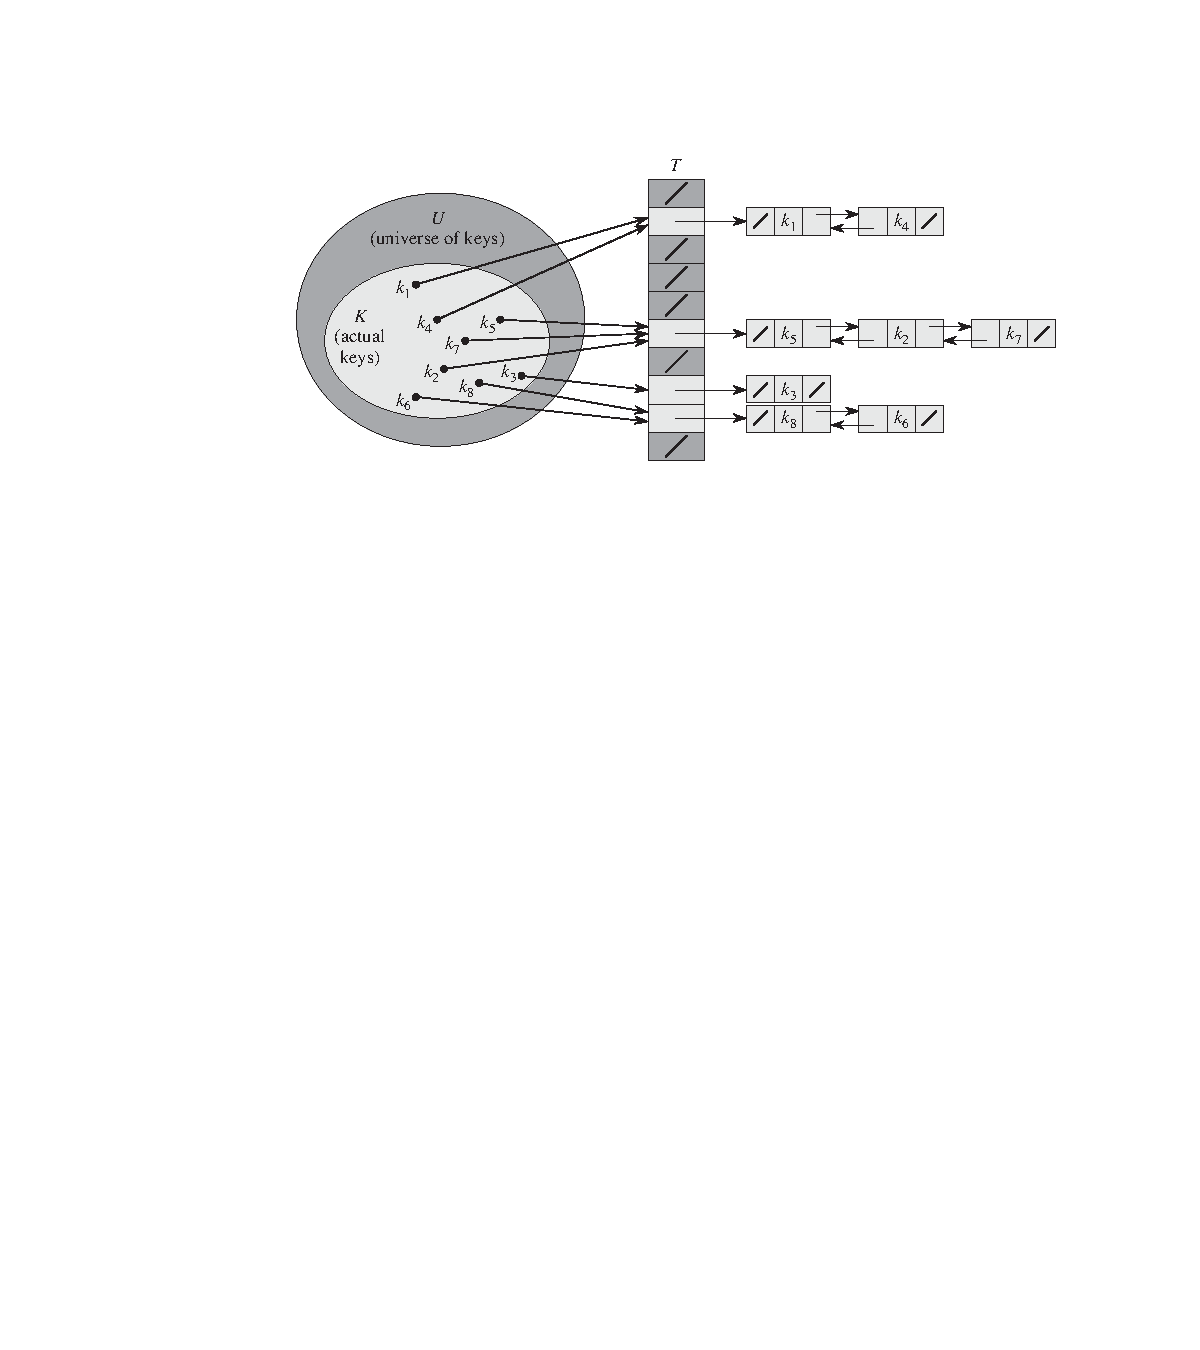
\includegraphics[width=0.8\textwidth]{aula05-hash1}
\caption{Exemplo de uma tabela hash com colisões.}
\label{aula05:fig:hash}
\end{figure}

O custo de busca para uma chave é $O(1 + \alpha)$ onde custo $1$ é aplicar
a função hash e acessar o slot, e $\alpha$ a busca na lista.
Então, o custo é $O(1)$ se $\alpha = O(1)$.

%%%%%%%%%%%%%%%%%%%%%%%%%%%%%%%%%%%%%%%%%%%%%%%%%%%%%%%%%%%%%%%%%%%%%%%%%%%%%%%%
\subsection{Endereçamento aberto}

No {\bf endereçamento aberto} todas as chaves são armazenadas na própria 
tabela, sem uso de memória adicional.
Se o endereço $e$ estiver ocupado tenta no endereço $e+1, e+2, ... n, 1, 2, ...  e-1$.

% TODO exemplo ziviane pg 86
Entre as várias propostas, a mais simples é \emph{hashing linear} dada por
\begin{equation*}
k(k,i) = (h'(k) + i)\; mod \; m.
\end{equation*}
O hashing linear sofre do {\bf agrupamento} (\emph{clustering}) na medida
em que a tabela começa a ficar cheia, pois a inserção de uma nova chave tende
a ocupar uma posição na tabela que esteja contígua a outras posições já ocupadas,
o que deteriora o tempo necessário para novas pesquisas.
Mesmo que o hashing linear ter esse problema, os resultados são satisfatórios.
O melhor caso, assim como o caso médio é $O(1)$.
O pior caso é $O(n)$.

%%%%%%%%%%%%%%%%%%%%%%%%%%%%%%%%%%%%%%%%%%%%%%%%%%%%%%%%%%%%%%%%%%%%%%%%%%%%%%%%
\subsection{Chaves não númericas}

As chaves não númericas devem ser transformadas em números dado por
\begin{equation*}
k = \sum_{i = 1}^{n} chave[i] \times p[i]
\end{equation*}
onde $n$ é o número de caracteres da chave, $chave[i]$ é o código ASCII do $i-$ésimo
caractere da chave, e $p[i]$ é um inteiro de um conjunto de pesos gerados aleatóriamente
para $1 \leq i \leq n$.

O uso de pesos tem a vantagem de gerar duas funções $h_1(k)$ e $h_2(k)$ diferentes
para dois conjuntos diferentes $p_1[i]$ e $p_2[i]$ $1 \leq i \leq n$.

%%%%%%%%%%%%%%%%%%%%%%%%%%%%%%%%%%%%%%%%%%%%%%%%%%%%%%%%%%%%%%%%%%%%%%%%%%%%%%%%
\subsection{Hashing perfeito}

Se $h(x_i) = h(x_j)$ se e somente se $i = j$, então não há colisões e a 
função de transformação é chamada de {\bf função de transformação perfeita}.
Se o número de chaves $n$ e o tamanho da tabela $m$ são iguais, então temos uma
{\bf função de transformação perfeita mínima} ($hp$).

Se $x_i \leq x_j$ e $hp(x_i) \leq hp(x_j)$ então a ordem lexicográfica é preservada. 
Nesse caso, temos uma {\bf função de transformação perfeito mínima com ordem preservada}.

%%%%%%%%%%%%%%%%%%%%%%%%%%%%%%%%%%%%%%%%%%%%%%%%%%%%%%%%%%%%%%%%%%%%%%%%%%%%%%%
\section{Busca digital}
%%%%%%%%%%%%%%%%%%%%%%%%%%%%%%%%%%%%%%%%%%%%%%%%%%%%%%%%%%%%%%%%%%%%%%%%%%%%%%%

A busca digital, ou pesquisa digital, é baseada na representação das chaves como uma 
sequência de caracteres ou dígitos.
Em vez de comparar uma chave de busca com os elementos, os caracteres da chave
de busca são comparados.
O método de busca digital é análogo à pesquisa manual em dicionários.

Os métodos de busca digital são vantajosos quando as chaves são grandes e de 
\textbf{tamanho variável}.
Um aspecto interessante quanto aos métodos de pesquisa digital é a possibilidade
de localizar todas as ocorrências de uma determinada cadeia em um texto com tempo
de resposta logarítmico em relação ao tamanho do texto.

Os métodos estudados são Trie e Patricia.

%%%%%%%%%%%%%%%%%%%%%%%%%%%%%%%%%%%%%%%%%%%%%%%%%%%%%%%%%%%%%%%%%%%%%%%%%%%%%%%%
\subsection{Árvores Trie}

O nome \textbf{Trie} vem de \emph{Retrieval} (recuperação).
Uma trie é uma árvore de busca $n-$ária, o grau equivale ao tamanho do
alfabeto, e ordenada, cujos nós irmãos são ordenados.
Usada para indexar chaves de busca, em geral caracteres, os arcos
os arcos são caracteres da chave.

Considerando as chaves como sequência de bits (quando $n = 2$), o algoritmo
de pesquisa digital é semelhante ao de pesquisa em árvore, exceto que em vez de
caminhar na árvore de acordo com o resultado da comparação entre chaves, caminha-se
de acordo com os bits da chave.

A figura~\ref{aula05:fig:trie1} ilustra um exemplo de árvore Trie com palavras indexadas
Alma, Almir, Alto, Be, Cal.
%
\begin{figure}[ht]
\centering
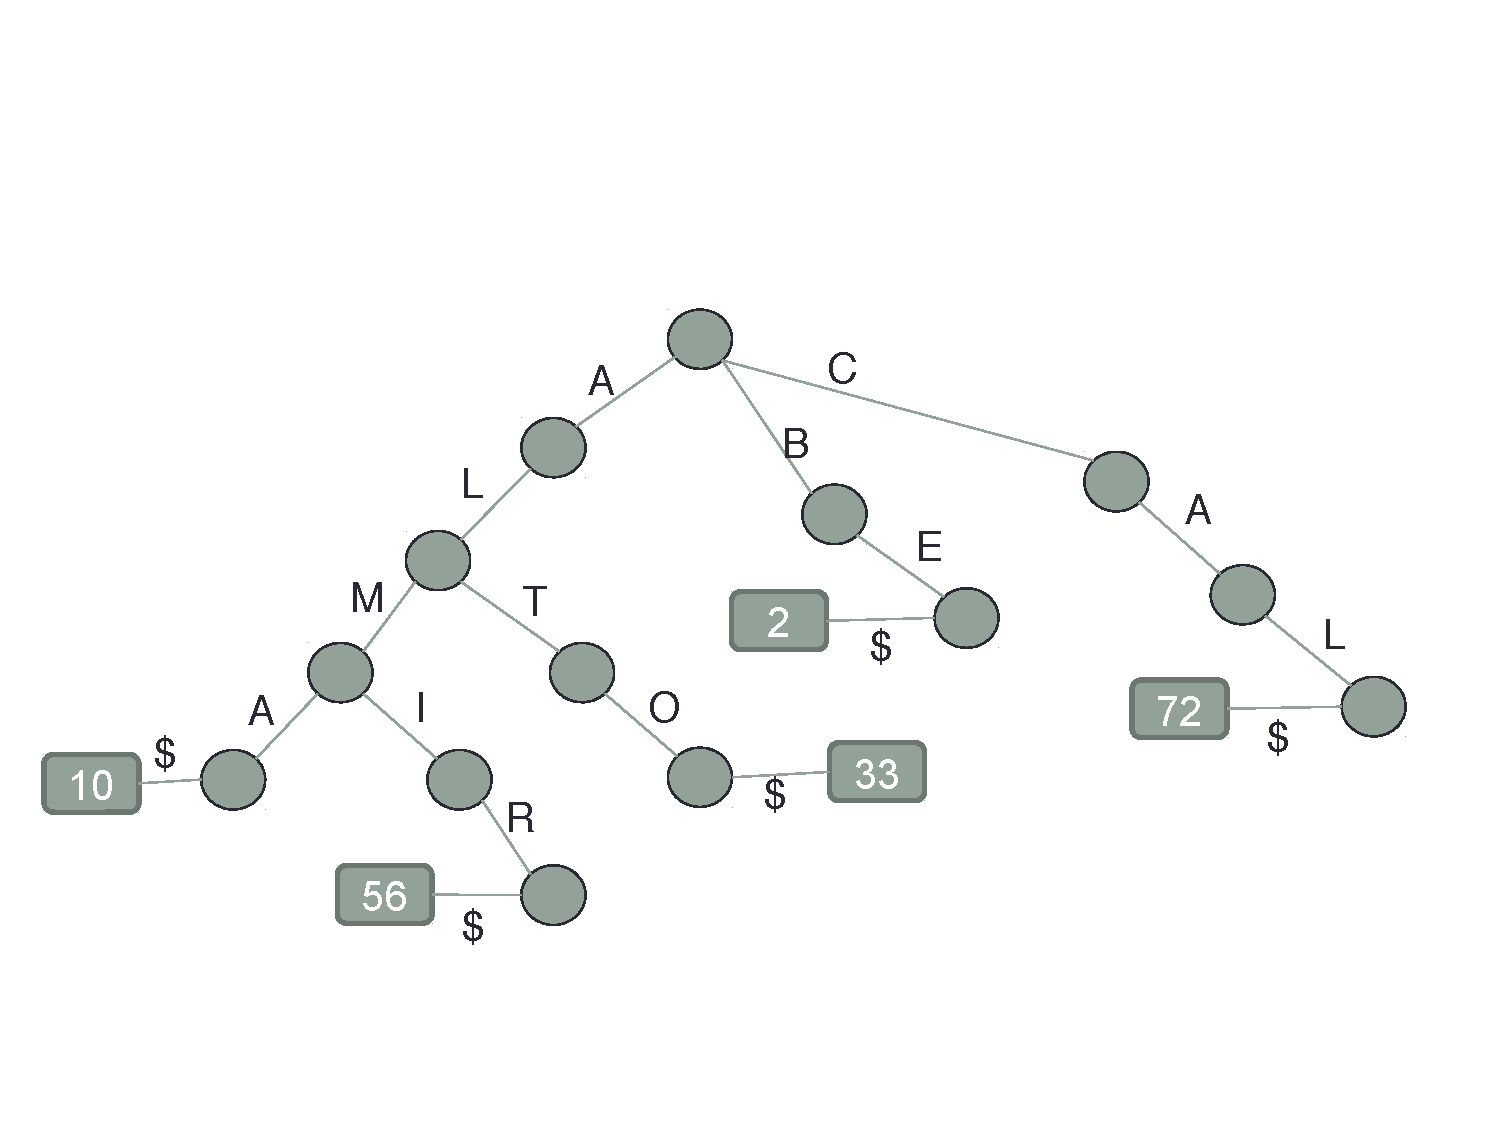
\includegraphics[width=0.7\textwidth]{aula05-trie1}
\caption{Exemplo de uma árvore Trie.}
\label{aula05:fig:trie1}
\end{figure}

\subsubsection{Chaves}

Uma chave é uma palavra sobre um alfabeto. 
Um símbolo é usado para indicar o término de uma chave. 
Esse símbolo deve ser um caractere que não faça parte do alfabeto, e garante
que uma chave não seja um prefixo de outra.
Dessa forma, os registros estarão nos nós folha da árvore.
%
\begin{description}
\item[Exemplo 1] tendo o alfabeto \{A, B, C, ..., Z\} e o símbolo
de término \$. Possíveis chaves: BOTA\$, CARRO\$, LEI\$.

\item[Exemplo 2] tendo o alfabeto \{0, 1, ..., 9\} e o símbolo de término \$.
Possíveis chaves: 134\$, 12978\$, 99777\$.
\end{description}
O caminho da raiz até um nó qualquer forma de um prefixo de uma chave indexada.

O formato das tries não depende da ordem em que as chaves são inseridas, depende
apenas dos valores das chaves.

\subsubsection{Estrutura de uma Trie}

A estrutura é composta de:
\begin{description}
\item[Nó raiz]  vazio e indexa nós que representem prefixos das chaves indexadas.
\item[Nós intermediários] prefixos de chaves de busca indexadas. Indexam outros nós
que aumentam o prefixo.
\item[Nós folha] chave completa e indexam as regiões de interesse. Ex.: offset da chave
de busca dentro de um arquivo de texto.
\end{description}

\subsubsection{Busca}

A busca começa pela raiz e pelo primeiro caractere.
Há dois cenários:
\begin{description}
\item[Cenário 1] o nó atual não é folha.
	\begin{enumerate}
	\item Se existe um filho que corresponda ao próximo caractere da chave.
		\begin{itemize}
		\item Avançar um caractere (passar a ignorá-lo a partir deste momento).
		\item Visitar o filho.
		\end{itemize}
	\item Se não existe esse filho.
		\begin{itemize}
		\item A chave não está indexada.
		\end{itemize}
	\end{enumerate}
\item[Cenário 2]  o nó atual é folha.
	\begin{enumerate}
	\item Esse nó de dados representa a resposta.
	\end{enumerate}
\end{description}

\subsubsection{Inserção}

Os passos da inserção são:
\begin{enumerate}
\item A palavra é buscada.
\item Se encontrar a palavra.
	\begin{enumerate}
	\item Adiciona-se um ponteiro no nó correspondente. O nó vira uma lista invertida contendo
	os offsets.
	\end{enumerate}
\item Caso contrário 
	\begin{enumerate}
	\item Localizar o último nó visitado.
	\item a partir desse nó, inserir o restante dos caracteres em novos nós.
	\end{enumerate}
\end{enumerate}

\subsubsection{Implementação}

Uma Trie pode ser implementada de duas formas diferentes:
\begin{itemize}
\item \textbf{R-Way} com nós de desvio e nós de informação. Os nós de desvio contem um filho para
cada símbolo do alfabeto mais um filho para o símbolo especial.

\item {\bf árvore TST (Ternary Search Tree)} ocupam menos espaço.
Cada nós possui um caractere e três ponteiros: próximo caractere (centro), 
caractere alternativo menor que o atual (esquerda), e caractere alternativo
maior que o atual (direita).
\end{itemize}

\subsubsection{Análise}

O custo em execução é $O(k m)$ para $k$ o tamanho do alfabeto e $m$ o tamanho da 
chave de busca.
O tempo de execução é independente do número de chaves, e a altura é igual ao comprimento da chave
mais longa.

O custo em espaço é $O(s)$ para $s$ a soma do tamanho de todas as chaves. 

\subsubsection{Trie compacta}

O espaço de uma Trie é reduzido por meio de compressão de nós redundantes, ou seja,
mesclando nós que possuem apenas um caminho possível.
A figura~\ref{aula05:fig:trie2} ilustra a versão compacta da  árvore Trie 
da figura~\ref{aula05:fig:trie1}.
%
\begin{figure}[ht]
\centering
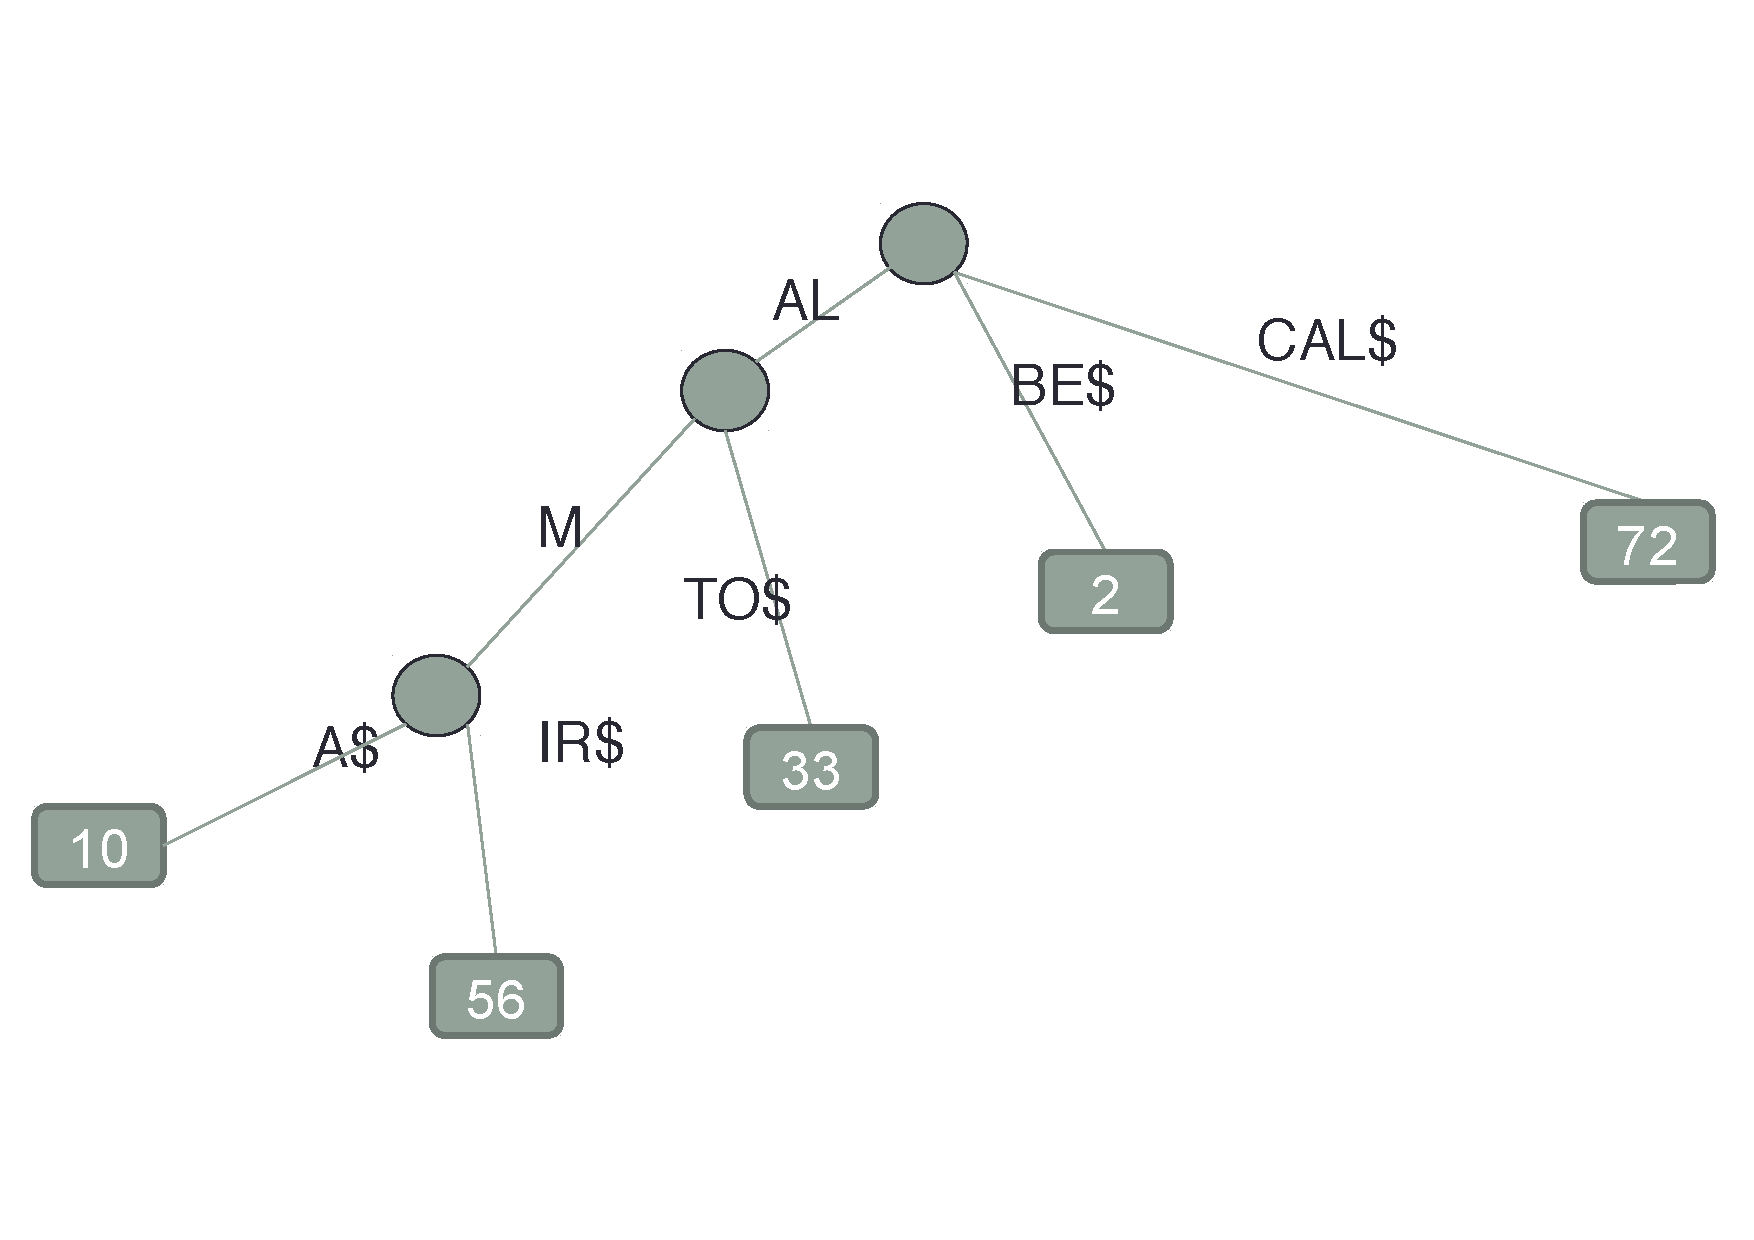
\includegraphics[width=0.6\textwidth]{aula05-trie2}
\caption{Exemplo de uma árvore Trie compacta.}
\label{aula05:fig:trie2}
\end{figure}

O custo em espaço de uma Trie compacta é $O(n)$ para $n$ o número de chaves, bem menor
que $O(s)$ da árvore não compacta. 
Todavia, o tempo de execução é o mesmo sendo $O(k m)$ para $k$ o tamanho do alfabeto e $m$
o tamanho da chave de busca.

\subsubsection{Trie binária}

Uma Trie binária é um tipo especial de Trie em que o alfabeto possui apenas 
apenas dois símbolos: \{0, 1\}.
Para compensar a ausência de símbolo especial, todas as cadeias de bits devem
ter o mesmo tamanho.
Caso alguma chave não tenha tamanho suficiente, basta preencher com 0s à
esquerda.

A figura~\ref{aula05:fig:trie3} ilustra um exemplo de árvore de árvore Trie binária
normal (esquerda) e compacta (direita) para os seguintes elementos:
\begin{itemize}
\item 0 - chave 000 valor 4.
\item 1 - chave 001 valor 22.
\item 4 - chave 100 valor 14.
\item 5 - chave 101 valor 39.
\end{itemize}
%
\begin{figure}[!htb]
\centering
  \begin{minipage}{0.4\textwidth}
	\centering
	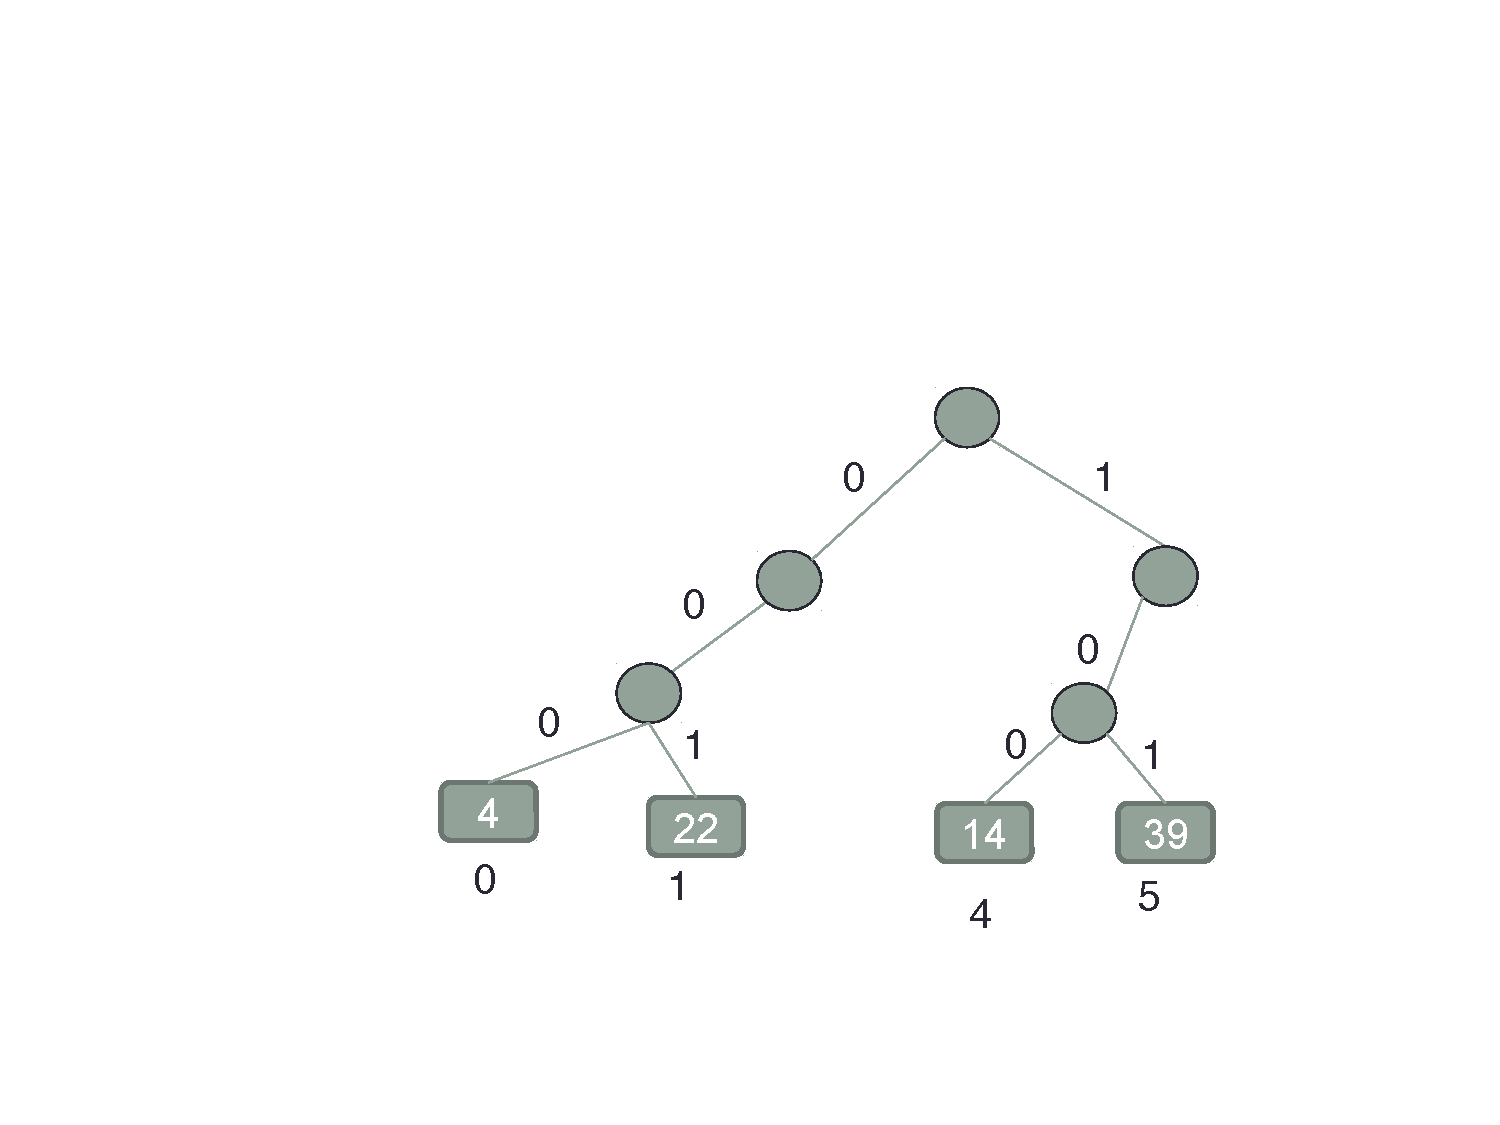
\includegraphics[width=\textwidth]{aula05-trie3}
  \end{minipage}
  %
  \vline
  %
  \begin{minipage}{0.4\textwidth}
	\centering
	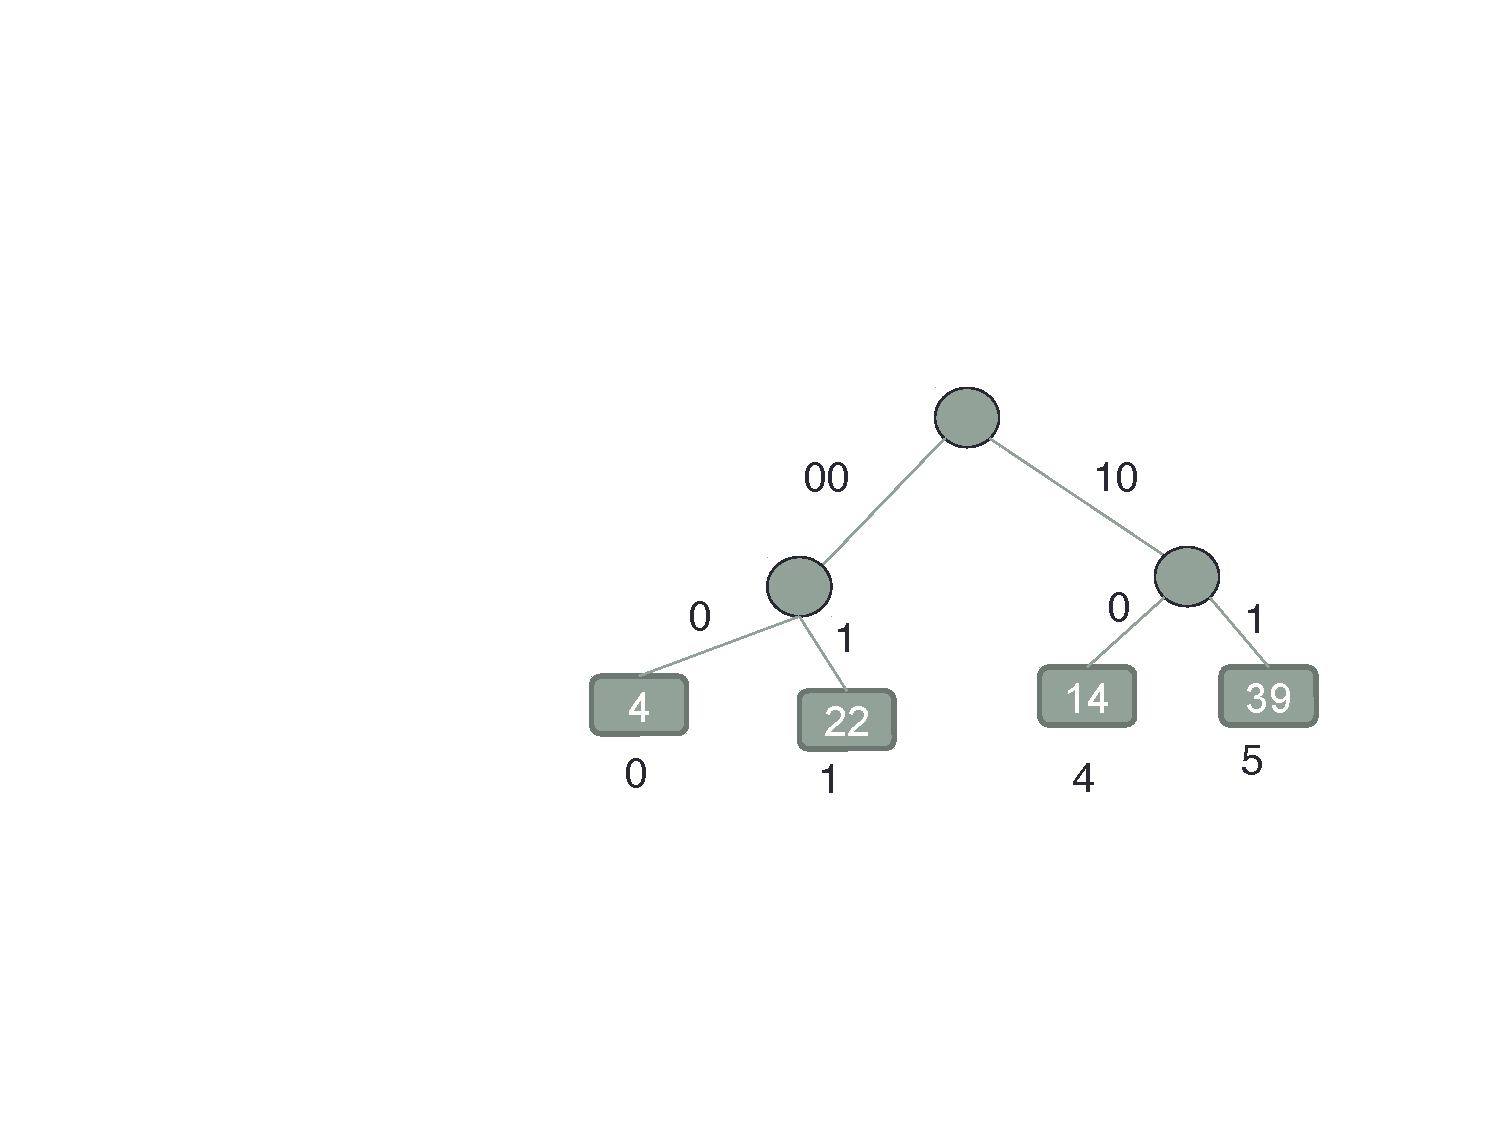
\includegraphics[width=\textwidth]{aula05-trie4}
  \end{minipage}
\caption{Exemplo de uma árvore Trie binária (esquerda) e binária compacta (direita).}
\label{aula05:fig:trie3}
\end{figure}

No pior caso, há $b$ comparações de bits, o que pode ser ineficiente quando as
chaves são grandes.  A versão compacta pode reduzir o custo, mas não o
suficiente.

%%%%%%%%%%%%%%%%%%%%%%%%%%%%%%%%%%%%%%%%%%%%%%%%%%%%%%%%%%%%%%%%%%%%%%%%%%%%%%%%
\subsection{Árvores Patricia}

Uma árvore Patricia, ou \emph{radix tree}, ou \emph{patricia trie}, vem do
acrônimo ``\emph{Practical Algorithm To Retrieve Information Coded In
Alphanumeric}'' e é uma árvore de busca compacta semelhante a uma Trie binária,
com alfabeto \{0, 1\}.
Entretanto, ela não usa um caractere especial para término (\$).
Todas as cadeias devem ter o mesmo tamanho.

Cada nó possui no máximo 2 filhos, e cada nó tem dois tipos: nós de desvio e nós de conteúdo.
Os nós de desvio possuem uma informação numérica que indica o bit da chave a testar.
A partir desse bit é decidido qual caminho da árvore a seguir.

A figura~\ref{aula05:fig:patricia1} mostra um exemplo de árvore Patricia e as
respectivas chaves.
Os valores dentro de cada nó indicam qual bit a ser testado no próximo desvio.
%
\begin{figure}[!htb]
\centering
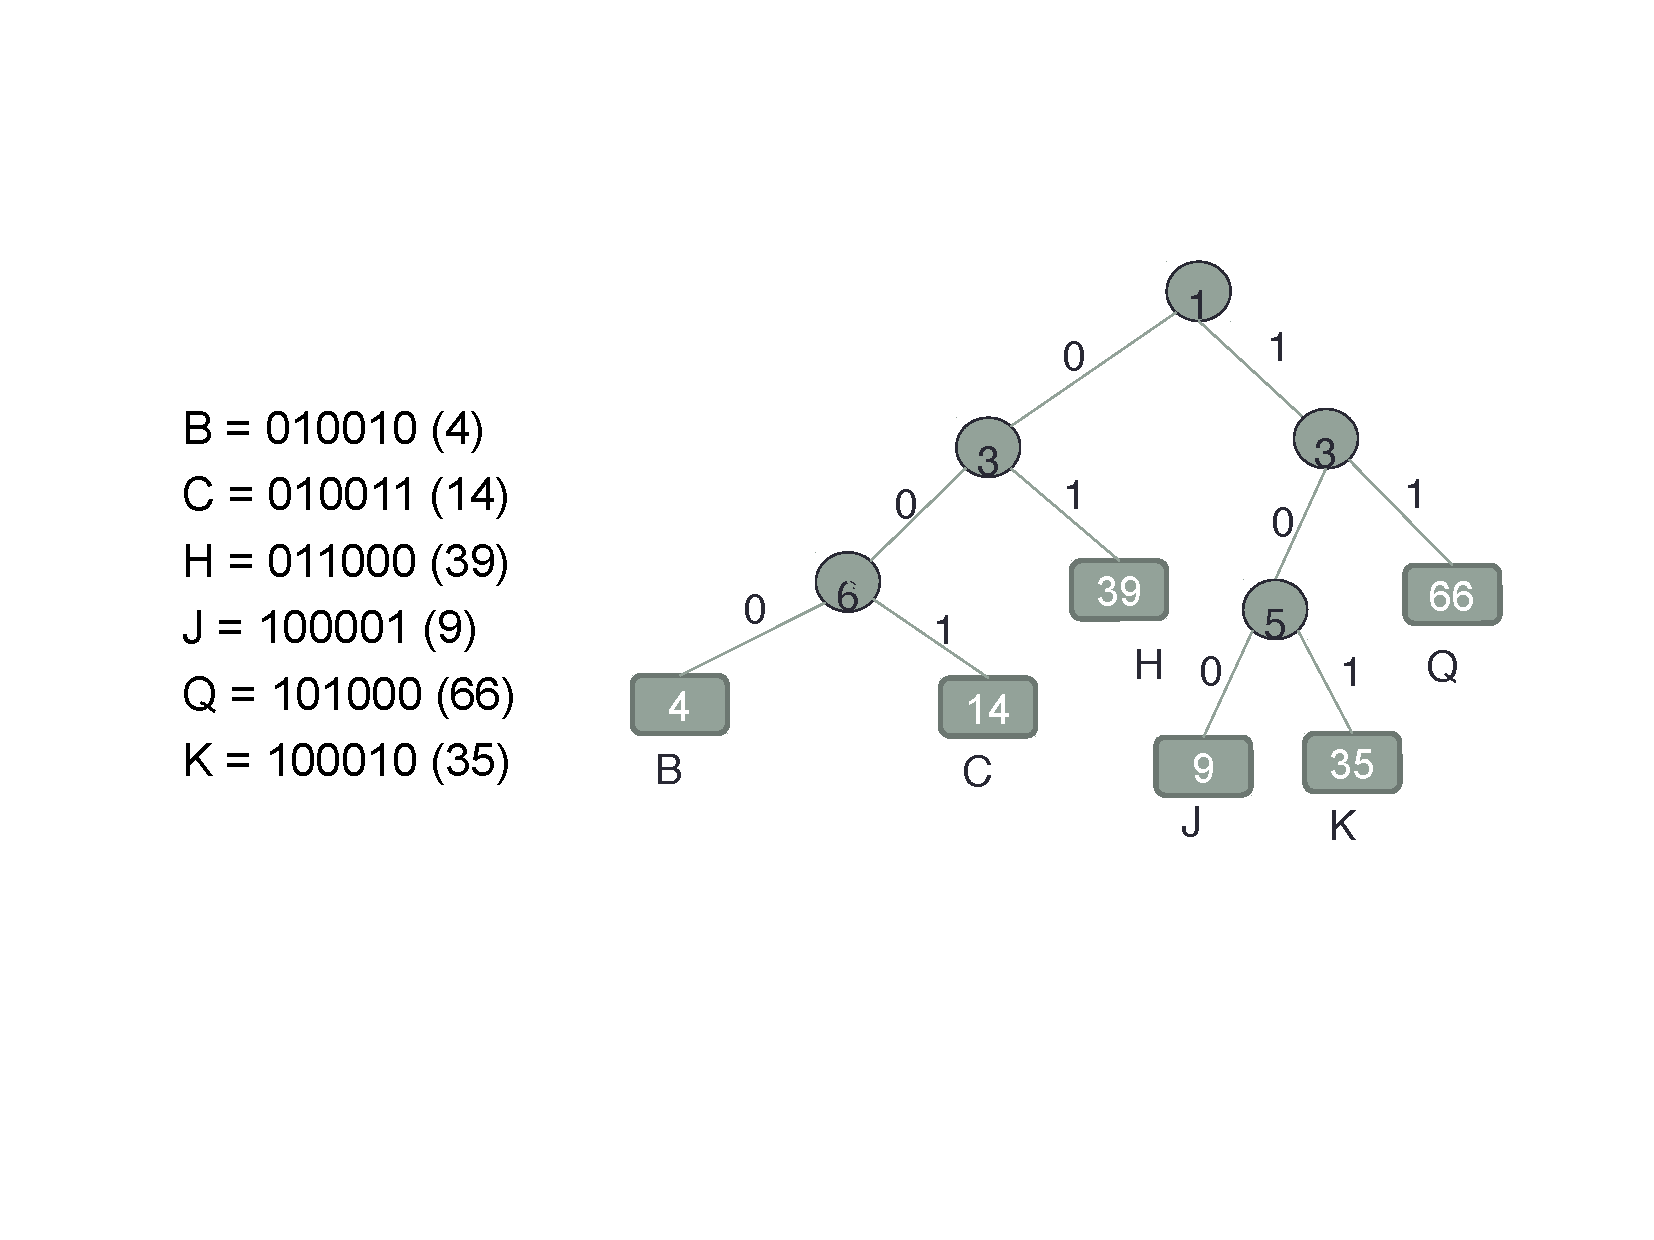
\includegraphics[width=0.6\textwidth]{aula05-patricia1}
\caption{Exemplo de uma árvore Patricia.}
\label{aula05:fig:patricia1}
\end{figure}

\subsubsection{Busca}

A busca começa pela raiz e pelo primeiro caractere (bit 0). 
Há dois cenários:
\begin{description}
\item[Cenário 1] o nó atual não é folha.
	\begin{enumerate}
	\item Verificar o dígito da chave de busca equivalente ao valor do nó.
	\item Se for 0, seguir a subárvore da esquerda.
	\item Caso contrário, seguir a subárvore da direita.
	\item Se não houver subárvore a seguir, a chave de busca não está indexada.
	\end{enumerate}

\item[Cenário 2] o nó atual é folha.
	\begin{enumerate}
	\item Deve-se verificar se o valor indexado realmente corresponde a chave de busca.
	\end{enumerate}
\end{description}

\subsubsection{Inserção}

Os passos da inserção em árvores Patricia são os seguintes:
\begin{enumerate}
\item A palavra (cadeia de bits) é buscada.
\item Se a árvore estiver vazia:
	\begin{enumerate}
	\item Cria-se uma estrutura inicial para indexar a palavra.
	\item Um nó raiz, com valor igual a 1, e um nó filho (a esquerda ou direita), indexando
		a palavra.
	\end{enumerate}
\item Se a busca parar em um nó anterior a um nó folha.
	\begin{enumerate}
	\item Significa que o nó só possui um único filho.
	\item Cria-se o outro filho, que indexará a palavra inserida.
	\end{enumerate}

\item Se a busca parar em um nó folha.
	\begin{enumerate}
	\item o conteúdo indexado é comparado com a palavra a ser inserida.
	\item se for igual, é adicionada uma entrada no nó folha para a palavra indexada.
	\item Se for diferente.
		\begin{enumerate}
		\item é preciso descobrir o nó da árvore a ser atualizado.
		\item para isso, é verificada a posição $P$ do primeiro bit onde ocorre a
			diferença.
		\item Se o bit for {\bf maior} que a última posição utilizada, deve-se adicionar um nó aqui.
		\item Se o bit for {\bf menor}  que a última posição utilizada, deve-ser subir na árvore
			para encontrar o local adequado. 
		\end{enumerate}
	\end{enumerate}

\item Para o caso de subida na árvore.
	\begin{enumerate}
	\item Sobe-se na árvore até encontrar o nó $X$, o nó mais baixo cujo
		valor seja maior que a posição $P$.
	\item Nesse ponto é inserido um novo nó, tendo como filhos:
		\begin{enumerate}
		\item O nó $X$.
		\item Um novo nó para indexar a nova palavra.
		\end{enumerate}
	\item Os ponteiros e valores dos nós criados/remanejados são atualizados.
	\end{enumerate}
	
\end{enumerate}

%%%%%%%%%%%%%%%%%%%%%%%%%%%%%%%%%%%%%%%%%%%%%%%%%%%%%%%%%%%%%%%%%%%%%%%%%%%%%%%%
\subsection{Aplicações de Tries e Patricia}

As Tries de caracteres podem ser aplicadas em:
\begin{itemize}
\item Verificadores de ortografia.
\item Motores de busca - nós folhas guardam páginas que possuem a palavra indexada.
\end{itemize}

As Tries binárias são usadas na compressão de dados, como na Codificação de Huffman.

As árvores Patricia podem ser usadas na indexação de chaves longas.

%%%%%%%%%%%%%%%%%%%%%%%%%%%%%%%%%%%%%%%%%%%%%%%%%%%%%%%%%%%%%%%%%%%%%%%%%%%%%%%
\section{Exercícios}
%%%%%%%%%%%%%%%%%%%%%%%%%%%%%%%%%%%%%%%%%%%%%%%%%%%%%%%%%%%%%%%%%%%%%%%%%%%%%%%

\begin{enumerate}
\item Descreva os passos da busca binária e os custos para o melhor caso, caso médio
e pior caso.

\item Qual é a principal característica de uma árvore binária de pesquisa ?

\item Descreva a árvore binária de busca criada a partir dos seguintes elementos:
$5, 8, 3, 6, 7, 1, 9, 4$.

\item A partir da árvore do exercício anterior, descreva a árvore binária de busca
resultante da remoção dos seguintes elementos: $4, 5$.

\item Desenhe a árvore AVL resultante da inserção dos números: 
$9, 8, 7, 6, 5, 4, 3, 2, 1$.

\item Escreva o algoritmo para imprimir o \textsc{menor} elemento de uma árvore de busca binária.
\item Escreva o algoritmo para imprimir o \textsc{maior} elemento de uma árvore de busca binária.

\item Escreva dois algoritmos que recebem uma árvore AVL como entrada: para
imprimir todos os elementos em ordem crescente e decrescente.

\item Considere a seguinte lista de valores: $[0, 9, 10, 3, 8, 4, 5, 1]$. 
	\begin{enumerate}
	\item Construa  uma árvore binária de busca não balanceada.
	\item Construa  uma árvore AVL.
	\end{enumerate}

\item Para uma árvore binária de busca:
	\begin{enumerate}
	\item Descreva um algoritmo {\bf não recursivo} que faz um percurso em-ordem.
	\item Descreva algoritmos recursivos para percursos pré-ordem e pós-ordem.
	\item Descreva algoritmos recursivos para buscar o elemento mínimo
		(\lstinline{ArvoreMinimo}) e elemento máximo
		(\lstinline{ArvoreMaximo}).
	\end{enumerate}

\item  Supondo que temos números de $1$ a $1000$ em uma árvore binária de busca,
e queremos buscar o número $363$. Quais das sequencias abaixo {\bf não} 
poderiam ser sequencias de nós percorridos nessa busca ?
	\begin{enumerate}
	\item $2,252,401,398,330,344,397,363$.
	\item $924, 220, 911, 244, 898, 258, 362, 363$.
	\item $925, 202, 911, 240, 912, 245, 363$.
	\item $2,399,387,219,266,382,381,278,363$.
	\item $935, 278, 347, 621, 299, 392, 358, 363$.
	\end{enumerate}

\item Desenhe uma árvore rubro-negra com chaves ${1, 2, ..., 15}$.
Adicione os nós folhas com \textsc{NIL} e faça coloração dos nós de forma
que o $bh(x)$ (\emph{black-height} ou altura-preto) da árvore seja 2, 3 e 4.

\item Mostre a árvore rubro-negra resultante depois de inserir sucessivamente
os nós ${41, 38, 31, 12, 19, 8}$ em uma árvore vazia.

\item Agora, baseado no exercício anterior,  mostre a árvore rubro-negra
resultante da remoção dos nós ${8, 12, 19, 31, 38, 41}$ sucessivamente.

\item Para as palavras chave da seguinte frase ``Marcos Lima marcou o marco'', e
	considerando o alfabeto \{a, b, ..., z\}, crie:
	\begin{enumerate}
	\item uma Trie compacta em formato de árvore.
	\item uma Trie normal, em formato R-Way.
	\item uma Trie normal, em formato TST.
	\end{enumerate}
Obs: artigos não precisma ser indexados.

\item Dadas as seguintes cadeias de bits: 00101 valor 5, 11000 valor 15, 01010 valor 34,
10101 valor 23, 11111 valor 12, 01110 valor 77. Crie:
	\begin{enumerate}
	\item uma Trie binária compacta.
	\item uma árvore Patricia.
	\end{enumerate}

\end{enumerate}

%%%%%%%%%%%%%%%%%%%%%%%%%%%%%%%%%%%%%%%%%%%%%%%%%%%%%%%%%%%%%%%%%%%%%%%%%%%%%%%
\chapter{Pesquisa em memória secundária}
%%%%%%%%%%%%%%%%%%%%%%%%%%%%%%%%%%%%%%%%%%%%%%%%%%%%%%%%%%%%%%%%%%%%%%%%%%%%%%%

Este capítulo aborda questões relacionadas a técnicas de armazenamento
e recuperação de dados em memória secundária.

%%%%%%%%%%%%%%%%%%%%%%%%%%%%%%%%%%%%%%%%%%%%%%%%%%%%%%%%%%%%%%%%%%%%%%%%%%%%%%%
\section{Memória secundária}
%%%%%%%%%%%%%%%%%%%%%%%%%%%%%%%%%%%%%%%%%%%%%%%%%%%%%%%%%%%%%%%%%%%%%%%%%%%%%%%

A classificação de dispositívos físicos pode ser feita ao considerar:
\begin{enumerate}
\item Desempenho no acesso aos dados.
\item Custo por unidade de dados.
\item Confiabilidade para casos de perda de dados em falhas de
energia ou falha do sistema, ou mesmo falha física do dispositívo.
\end{enumerate}
Também pode-se diferenciar armazenamento em:
\begin{description}
\item[Volátil] perde dados quando é desligado.
\item[Não-volátil] persistente mesmo quando é desligado. Inclui armazenamento
secundário e terciário.
\end{description}

%%%%%%%%%%%%%%%%%%%%%%%%%%%%%%%%%%%%%%%%%%%%%%%%%%%%%%%%%%%%%%%%%%%%%%%%%%%%%%%
\subsection{Mídias de armazenamento}

As médias de armazenamento disponíveis em geral são:
\begin{description}
\item[Cache] a mais rápida e custosa, volátil, e gerenciada pelo hardware
do processador.

\item[Memória principal] acesso rápido da ordem de 10 a 100 nanosegundos (1 nanosegundo = $10^{-9}$).
Em geral muito pequena (ou muito cara) para armazenar todos os dados de um banco de dados.
Hoje  em dia, em alguns casos, armazena todo o banco de dados (\emph{memcached}).
Ela é volátil, sendo que os dados são perdidos na falta de energia ou falha do sistema.

\item[Flash] dados sobrevivem em falhas de energia. Dados podem ser escritos em um local
uma única vez, porém podem ser escritos novamente.
Pode ser lida um número ilimitado de vezes, mas há um limite no  número de gravações
que varia entre 10K e 1M.
As leituras podem ser mais rápidas que a memória principal, mas as escritas
são lentas.
Muito usada em dispositivos embarcados como câmeras digitais, 
telefones, e memórias flash drive (pendrive).

\item[Magnética] dados são armazenados em uma mídia magnética com discos de movimento
giratório. 
Deve-se ler os dados do disco para a memória principal, e depois escrever de volta ao disco.
O acesso direto é possível em qualquer ordem, ao contrário de mídias de fita.


\item[Ótica] não volátil e os dados são lidos óticamente de um disco 
giratório através de um laser.
Os mais populares são CD-ROM (640 MB), DVD (4.7GB), e Blu-ray (27 GB a 54 GB).
As leituras e escritas são mais lentas comparadas a discos magnéticos.

\item[Fita magnética]
não volátil, usado primariamente para backup (recuperar falhas de disco), e 
arquivamento de dados.
O acesso é sequencial, muito mais lento que discos. Porém, a capacidade
de armazenamento é alta (40 a 300GB).
\end{description}

A figura~\ref{aula06:fig:media} ilustra a hierarquia de armazenamento de acordo com 
o desempenho e custo.
Os níveis mais altos são mais custosos, porém mais rápidos.
No sentido contrário, o custo por bit reduz, mas o tempo de acesso aumenta.
%
\begin{figure}[!htb]
\centering
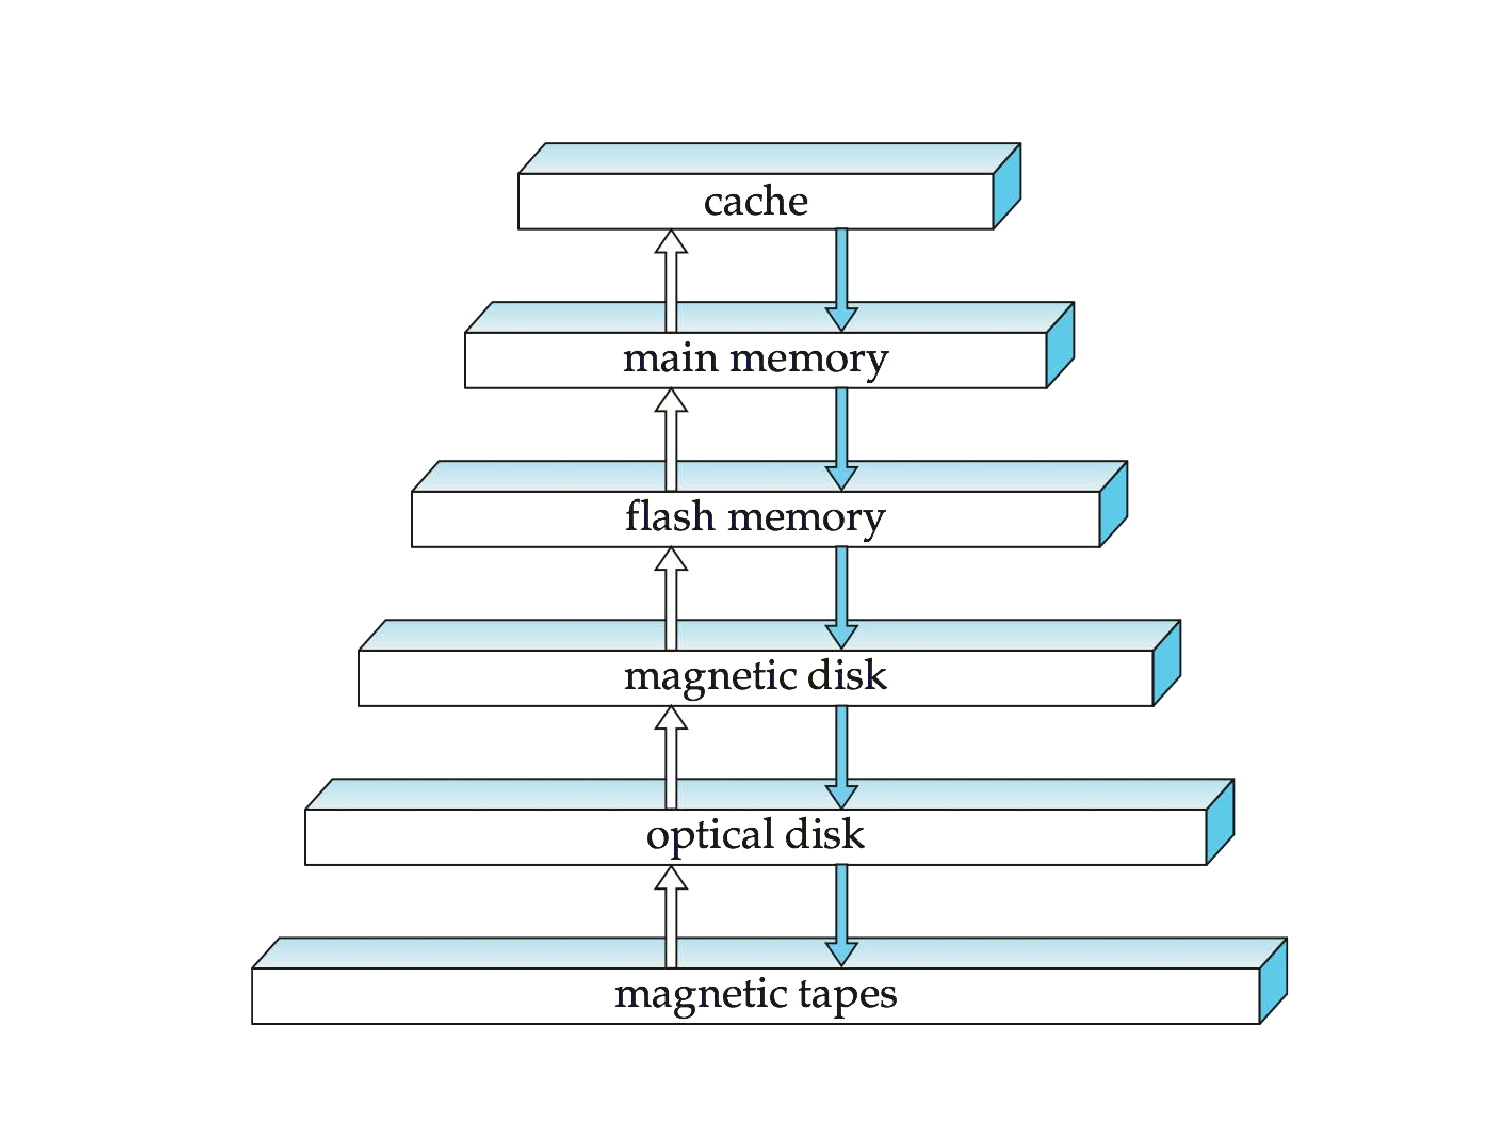
\includegraphics[width=0.6\textwidth]{aula06-media}
\caption{Hierarquia de mídias de armazenamento.}
\label{aula06:fig:media}
\end{figure}

Nessa hierarquia, podemos agrupar as mídias em:
\begin{description}
\item[Armazenamento primário] mais rápido mas volátil. Ex: cache, memória principal.

\item[Armazenamento segundário] próximo nível na hierarquia, não volátil,
acesso moderadamente rápido. Ex: memória flash, discos magnéticos.

\item[Armazenamento terciário] nível mais baixo, não volátil, tempo de acesso
lento. Também chamado armazenamento \emph{off-line}. Ex: fita magnética, armazenamento ótico.
\end{description}

%%%%%%%%%%%%%%%%%%%%%%%%%%%%%%%%%%%%%%%%%%%%%%%%%%%%%%%%%%%%%%%%%%%%%%%%%%%%%%%
\subsection{Disco magnético}

\subsubsection{Estrutura física}

Fisicamente, discos magnéticos são simples.
A figura~\ref{aula06:fig:hd} mostra o funcionamento interno de um disco.
%
\begin{figure}[!htb]
\centering
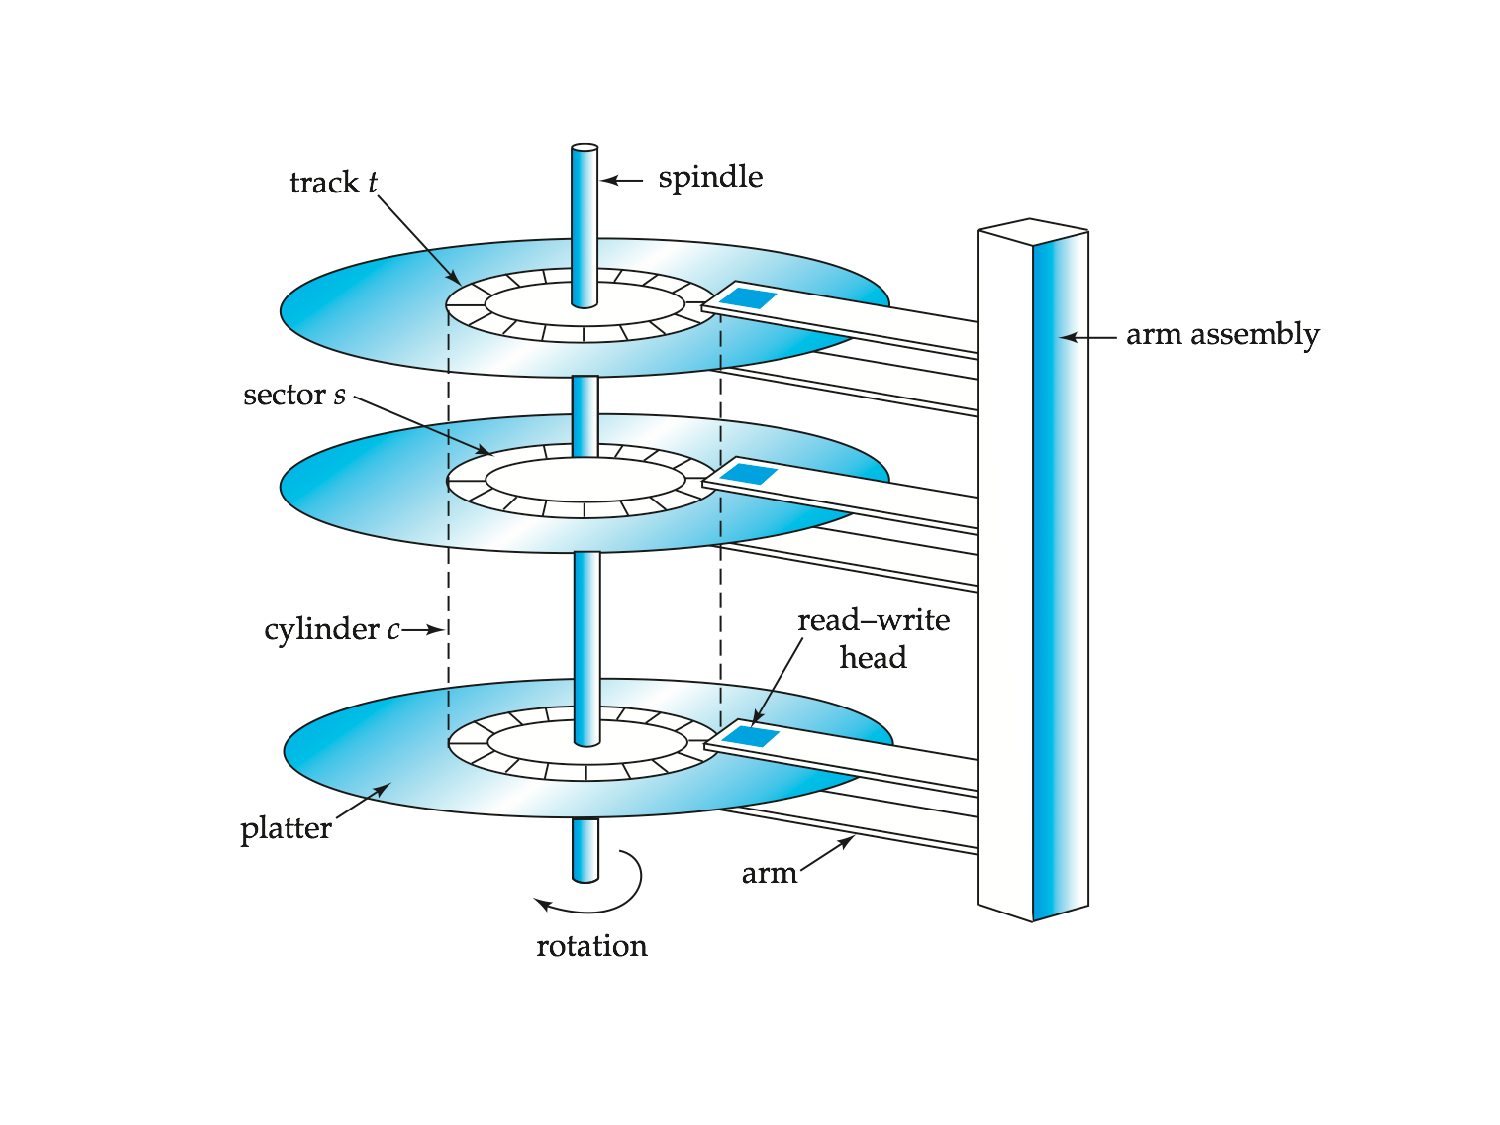
\includegraphics[width=0.6\textwidth]{aula06-hd}
\caption{Mecanismo de cabeças de leitura em um disco magnético.}
\label{aula06:fig:hd}
\end{figure}

Cada prato do disco tem duas superfícias com material magnético, onde a informação
é gravada.
O cabeçote de escrita-leitura (\emph{read-write head}) fica posicionada bem 
próxima a superfície do prato, e lê e escreve dados codificados magneticamente.
A superfície é dividida logicamente em {\bf trilhas}, que são subdivididas em 
\textbf{setores}. 
Um setor é a menor unidade que pode ser lida ou escrita do disco.
Em geral, um setor tem 512 bytes; há perto de 50K a 100K trilhas por prato, e 1
a 5 pratos por disco.

Os pratos são montados em braços de disco.
Para ler e escrever um setor, o braço do disco se move para posicionar o cabeçote
na trilha correta.
O prato gira, e os dados são lidos e/ou escritos a medida que o setor
passa pelo cabeçote.

Outro componente de discos é o {\bf controlador de disco} que faz a inteface 
entre o computador e o hardware do disco.
Ele aceita comandos de alto nível para ler e escrever setores.
Entre outras funções, garante checagem de erros.

\subsubsection{Medidas desempenho}

O \textbf{tempo de acesso} é o tempo que leva desde a solicitação de leitura/escrita
até o momento em que a transferência começa de fato. 
O tempo de acesso consiste em:
\begin{description}
\item[Tempo de busca] tempo que leva para reposicionar o braço na trilha correta.
O tempo médio de busca é 1/2 do pior tempo de busca, em geral 4 a 10 milisegundos.

\item[Latência rotacional] tempo que leva para o setor a ser acessado
aparecer debaixo do cabeçote. Latência média é 1/2 do pior caso, em geral
4 a 11 milisegundos em discos (5400 a 15000 rpm). 
\end{description}

A \textbf{taxa de transferência} é a taxa com que os dados são recuperados ou 
armazenados no disco. A taxa máxima é de 25 a 100 MB por segundo, e essa
taxa é menor para trilhas internas.

O \emph{Mean time to failure} (MTTF) é o tempo médio de funcionamento de um disco
sem falhas. 
Esse tempo varia entre 3 a 5 anos. 
A probabilidade de falhas em disco novos é baixa, que corresponde a um
``MTTF teórico'' de 500K a 1,2M horas.
Ou seja, um MTTF de 1,2M horas para um disco novo significa que dados 1000 novos discos,
na média um irá falhar a cada 1200 horas.

\subsubsection{Otimização de acessos}

A transferência de dados entre disco e memória ocorre em unidades de \textbf{blocos},
que são uma sequência continua de setores em uma única trilha.
O tamanho varia de 512 a vários kilobytes. Blocos pequenos podem implicar 
em várias transferencias do disco, enquanto que grandes blocos podem 
desperdiçar espaços devido a blocos parcialmente ocupados.
Um tamanho típico utilizado é de 4 a 16 kilobytes.

A otimização de acessos envolve \textbf{algoritmos de escalonamento} que são usados para ordenar o 
acesso às trilhas para minimizar o  movimento do braço.
O \textbf{algoritmo do elevador} funciona da seguinte forma:
\begin{enumerate}
\item move o braço do disco em uma direção (de dentro para fora ou de fora para dentro).
\item processa todas as requisições pendentes nessa direção.
\item reverte o movimento e repete a varredura.
\end{enumerate}

Outra forma de otimização é a \textbf{organização de arquivos} que otimiza o acesso ao
organizar os blocos, de modo a corresponder à forma com que os dados são acessados.
Exemplo é armazenar informações relacionadas em regiões próximas.
Arquivos podem se \textbf{fragmentar} com o passar do tempo.
Fragmentação acontece quando o arquivo é modificado, ou quando os blocos livres
estão espalhados, e novos arquivos tiverem que ocupar esses blocos.
O acesso sequencial a um arquivo fragmentado leva a maior movimentação do
braço do disco. 
Alguns sistemas possuem utilitários para \textbf{desfragmentar} o sistema
de arquivos, de modo a acelerar o acesso.

%%%%%%%%%%%%%%%%%%%%%%%%%%%%%%%%%%%%%%%%%%%%%%%%%%%%%%%%%%%%%%%%%%%%%%%%%%%%%%%
\section{Organização de arquivos}
%%%%%%%%%%%%%%%%%%%%%%%%%%%%%%%%%%%%%%%%%%%%%%%%%%%%%%%%%%%%%%%%%%%%%%%%%%%%%%%

A pesquisa em memória secundária normalmente está associada a \textbf{pesquisa 
em bancos de dados}.
O banco de dados é armazenado como uma coleção de arquivos. Cada arquivo
é uma sequência de registros, e cada registro é uma sequência de campos.

%%%%%%%%%%%%%%%%%%%%%%%%%%%%%%%%%%%%%%%%%%%%%%%%%%%%%%%%%%%%%%%%%%%%%%%%%%%%%%%
\subsection{Registros de tamanho fixo}

A estratégia mais simples é assumir \textbf{registros de tamanho fixo}.
Cada tabela possui o seu próprio arquivo, e cada arquivo possui registros
de um tipo específico de dado.
O cabeçalho possui informações de controle. Cada registro tem um ponteiro
especial, que aponta para o seu próximo registro.
O problema com essa abordagem é a ocupação parcial do bloco.
Por exemplo, cada registro ocupa 300 bytes e cada bloco ocupa 1024 bytes.
O cabeçalho ocupa 20 bytes. Qual o mínimo de espaço que será desperdiçado ?

Uma solução é permitir que registros cruzem a fronteira de um bloco. 
As alternativas para remoção do registro $i$ são:
\begin{enumerate}
\item mover registros $i+1$, ..., $n$ para $i$, ..., $n-1$.
\item mover registro $n$ para $i$.
\item não mover nada, ligar os registros vazios por uma \emph{free list}.
\end{enumerate}

Com \emph{free lists}, pode-se usar um ponteiro especial para guardar os registros livres.
Ela é uma representação mais eficiente que reusa o espaço destinado
aos atributos dos registros para guardar os ponteiros.
O cabeçalho possui informações de controle como ponteiro para o primeiro registro
com dados do bloco, e ponteiro para o primeiro registro livre do bloco.

O principal problema dessa abordagem é o desperdício de espaço dentro do bloco.

%%%%%%%%%%%%%%%%%%%%%%%%%%%%%%%%%%%%%%%%%%%%%%%%%%%%%%%%%%%%%%%%%%%%%%%%%%%%%%%
\subsection{Registros de tamanho variável}

A estrutura de \textbf{slotted-page} é comumente utilizada para organizar
registros de tamanho variável dentro de um bloco.
A figura~\ref{aula06:fig:slotted} ilustra a estrutura.
%
\begin{figure}[!htb]
\centering
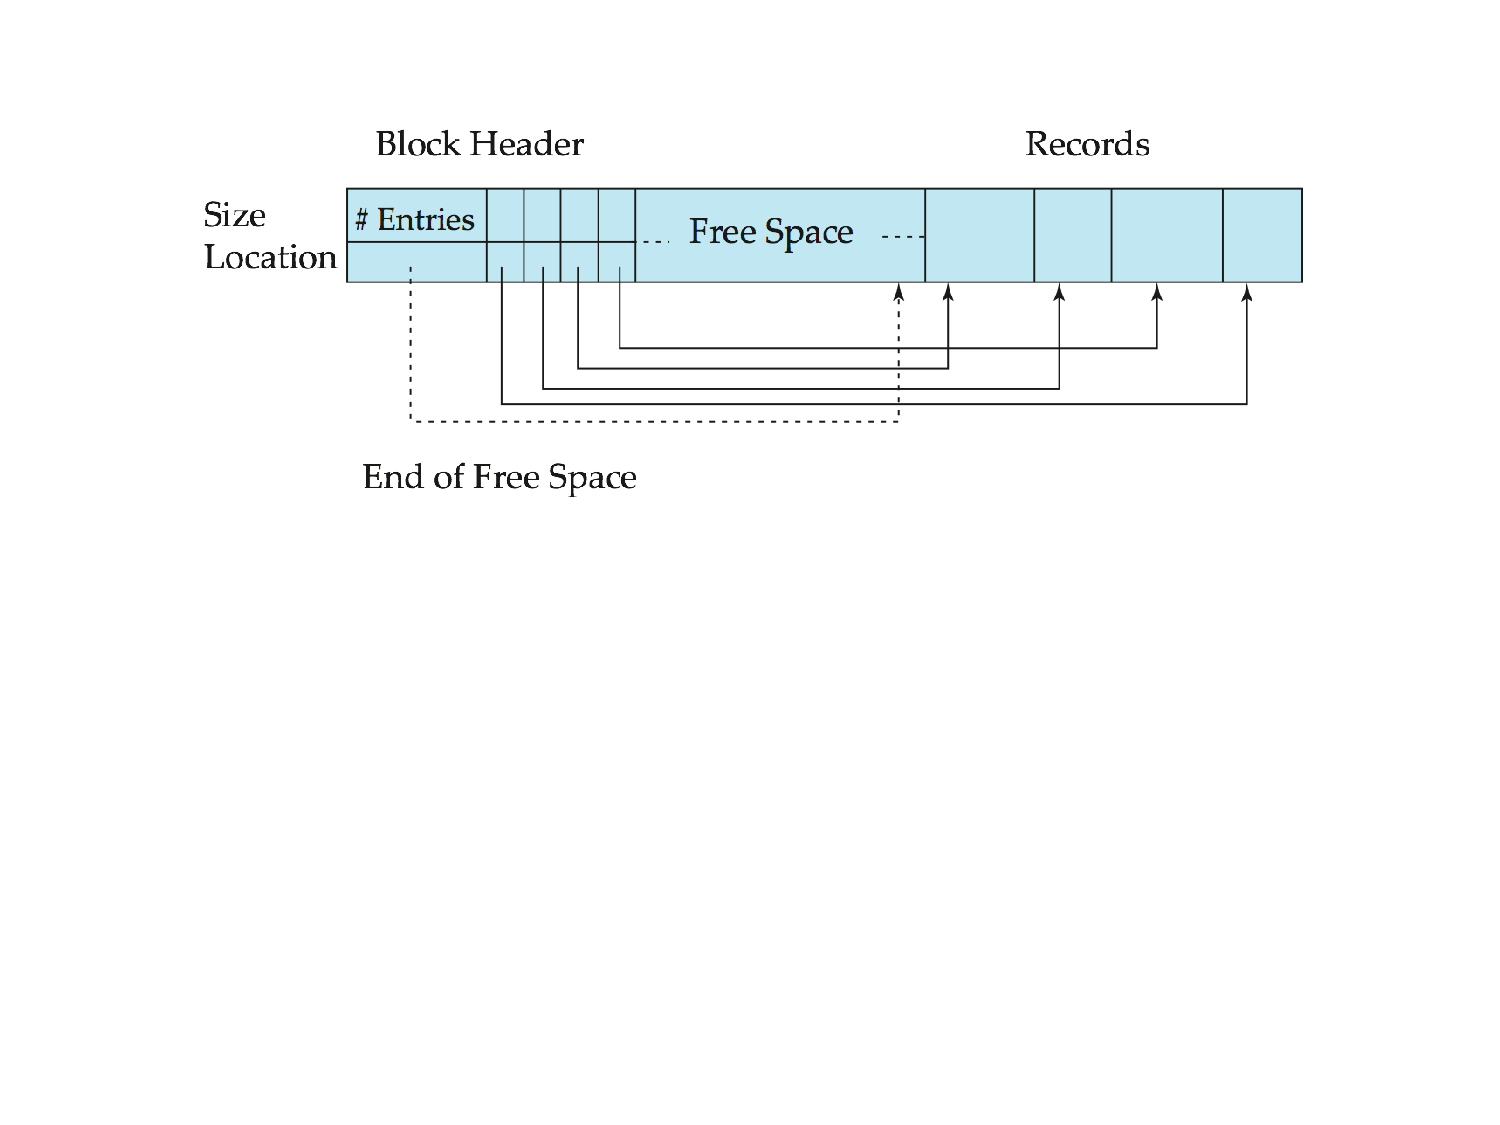
\includegraphics[width=0.8\textwidth]{aula06-slotted}
\caption{Estrutura do \emph{slotted-page}.}
\label{aula06:fig:slotted}
\end{figure}
O cabeçalho contém:
\begin{itemize}
\item número de registros.
\item localização e tamanho de cada registro.
\item fim do espaço livre no bloco.
\end{itemize}
Os registros podem ser movidos dentro de uma página para evitar espaços vazios
entre eles; as entradas no cabeçalho precisam ser atualizadas.
Ponteiros não apontam diretamente para o registro, mas apontam 
para o ponteiro de entrada do registro no cabeçalho.

Registros de tamanho variável aparecem em bancos de dados de diversas formas:
armazenameto de múltiplos tipos de conteúdo em um mesmo arquivo;
armazenamento de atributos que possuem tamanho variável.

Se as slotted-pages são do tamanho de um bloco, o problema dos registros que cruzam é eliminado.
Isso limita o tamanho dos registros em um banco de dados, o que é o caso padrão.

%%%%%%%%%%%%%%%%%%%%%%%%%%%%%%%%%%%%%%%%%%%%%%%%%%%%%%%%%%%%%%%%%%%%%%%%%%%%%%%
\section{Organização de registros em arquivos}
%%%%%%%%%%%%%%%%%%%%%%%%%%%%%%%%%%%%%%%%%%%%%%%%%%%%%%%%%%%%%%%%%%%%%%%%%%%%%%%

Até agora, vimos como representar registros em uma estrutura de arquivo.
Há várias formas de organizar registros em arquivos:
\begin{description}
\item[Heap] um registro pode ser posicionado em qualquer lugar onde haja espaço.

\item[Sequencial] registros armazenados em ordem sequencial, com base
no valor da chave de busca de cada registro.

\item[Hashing] um função hash calculada com base em alguns atributos do 
registro. O resultado especifica em que bloco do arquivo do registro
deve ser posicionado.
\end{description}

%%%%%%%%%%%%%%%%%%%%%%%%%%%%%%%%%%%%%%%%%%%%%%%%%%%%%%%%%%%%%%%%%%%%%%%%%%%%%%%
\subsection{Organização de arquivos sequencial}

Adequada para aplicações que executam processamento sequencial sobre todo o arquivo.
Os registros do arquivo são ordenados por uma \textbf{chave de busca}.

A operação de remoção usa \emph{free lists} para registros de tamanho fixo.

A inserção localiza a posição onde o registro deve ser inserido e:
\begin{enumerate}
\item se houver espaço no bloco, insere no bloco.
\item se for o último registro, insere em um novo bloco.
\item se houver espaço em um bloco vizinho, distribuir. Caso contrário,
insere em um novo \textbf{bloco de estouro} (\emph{overflow block}).
\item de qualquer forma, as cadeias de ponteiros precisam ser atualizadas.
\end{enumerate}
O uso de blocos de estouro demanda a reorganização do arquivo de tempo em tempo
para restaurar a ordem sequencial.

%%%%%%%%%%%%%%%%%%%%%%%%%%%%%%%%%%%%%%%%%%%%%%%%%%%%%%%%%%%%%%%%%%%%%%%%%%%%%%%
\subsection{Clusterização multitable}

Os registros de cada tabela podem ser armazenados em arquivos separados.
Em uma \textbf{clusterização multitable}, registros de tabelas diferentes são armazenados no mesmo 
arquivo.
A principal motivação para armazenar registros relacionados no mesmo bloco é minimizar
a entrada e saída.
A figura~\ref{aula06:fig:clustering1} ilustra a organização de um arquivo com clusterização.
Esse arquivo armazena registros de uma ou mais relações em cada bloco.
Tal organização permite a leitura de registros que podem satisfazer uma união por meio de 
uma leitura de bloco.
%
\begin{figure}[!htb]
\centering
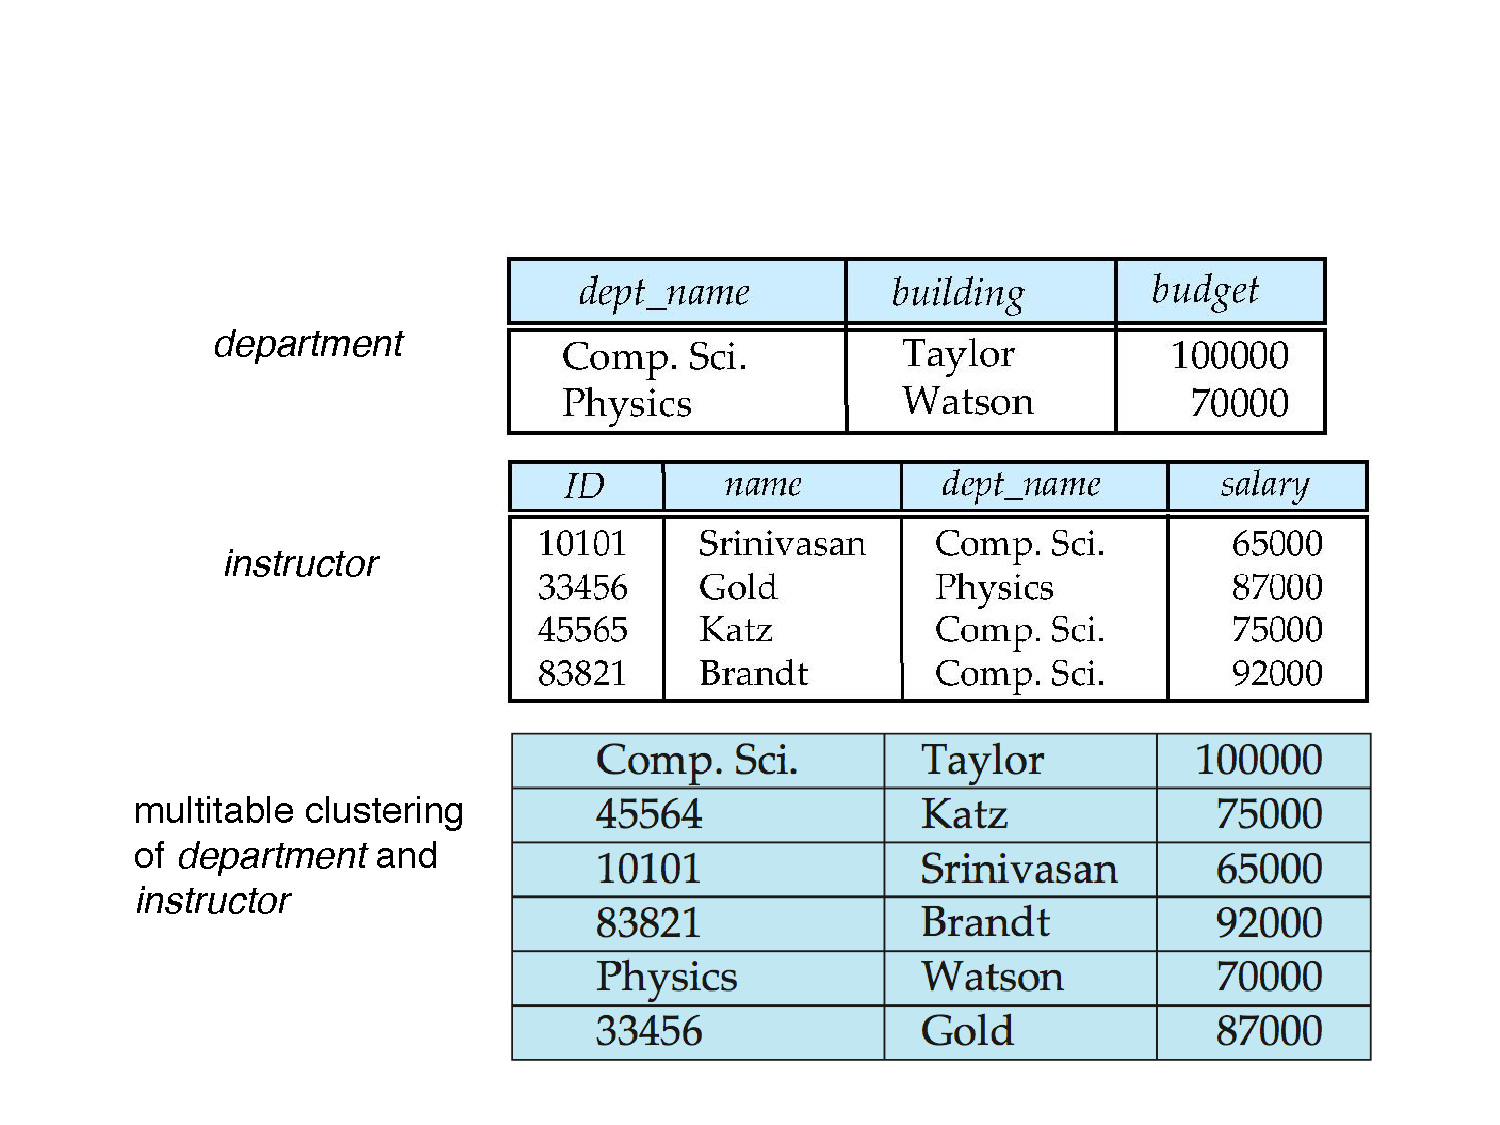
\includegraphics[width=0.6\textwidth]{aula06-clustering1}
\caption{Estrutura de arquivo de uma clusterização multitable.}
\label{aula06:fig:clustering1}
\end{figure}

Essa organização é boa para consultas com relação, e consultas envolvendo um único
deparamento e seus professores.
Porém, ela é ruim para consultas somente de departamentos.

%%%%%%%%%%%%%%%%%%%%%%%%%%%%%%%%%%%%%%%%%%%%%%%%%%%%%%%%%%%%%%%%%%%%%%%%%%%%%%%
\section{Sistemas de arquivos}
%%%%%%%%%%%%%%%%%%%%%%%%%%%%%%%%%%%%%%%%%%%%%%%%%%%%%%%%%%%%%%%%%%%%%%%%%%%%%%%

Em organizações de arquivos sequencias, cada tabela é armazenada em um arquivo.
O armazenamento poderia ser feito por meio do sistema de arquivos do sistema
operacional (SO).
A clusterização multitable pode trazer ganhos significativos em eficiência, mas 
essa organização não é compatível com o sistema de arquivos de sistemas operacionais.

Muitos dos sistemas de bancos de dados (SGBDs) de grande escala não utilizam diretamente o SO.
As tabelas são armazenadas em um único arquivo, e o SGBD gerencia o arquivos por conta própria.
Isso exige a implementação de um sistema de arquivos dentro do SGBD.

%%%%%%%%%%%%%%%%%%%%%%%%%%%%%%%%%%%%%%%%%%%%%%%%%%%%%%%%%%%%%%%%%%%%%%%%%%%%%%%
\subsection{Buffer manager}

O  número de transferencias de blocos entre o disco e a memória pode ser
reduzido mantendo o maior número possível de blocos na memória principal.
Um \textbf{buffer} é a porção da memória principal disponível para armazenar cópias
de blocos de disco.
O \textbf{buffer manager} é responsável pela alocação de espaço do buffer na 
memória principal.

Programas utilizam o buffer manager quando precisam ler um bloco do disco:
\begin{enumerate}
\item se o bloco já estiver no buffer, o gerenciador retorna o endereço 
do bloco na memória principal.

\item se o bloco não estiver no buffer, o manager:
	\begin{enumerate}
	\item aloca espaço no buffer para o bloco.
		\begin{enumerate}
		\item substituindo algum outro bloco, se necessário, para
			liberar espaço para o novo bloco.
		\item o bloco substituído é escrito de volta no disco somente se ele foi
		modificado desde a última vez que ele foi escrito/recuperado do disco.
		\end{enumerate}
	\item Lê o bloco do disco para o buffer e retorna o endereço do bloco
		na memóra principal para o programa.
	\end{enumerate}
\end{enumerate}

Sua função é similar ao gerenciamento e memória virtual dos sistemas operacionais.
Porém, bancos de dados tem requisitos diferentes.

%%%%%%%%%%%%%%%%%%%%%%%%%%%%%%%%%%%%%%%%%%%%%%%%%%%%%%%%%%%%%%%%%%%%%%%%%%%%%%%
\subsection{Políticas de substituição de blocos}

A maioria dos sistemas operacionais usam a política de substituição do bloco menos recentemente usado
ou \emph{least recently used} (LRU).
A ideia por trás do LRU é usar um padrão passado de referência a blocos como uma previsão de 
futuras referências, já que usualmente nada mais se conhece.
Consultas possuem um padrão de acesso bem definido, com varreduras sequenciais.
O sistema do BD pode usar informação contida na consulta para prever referências futuras.

O LRU pode ser uma estratégia ruim para certos tipos de acesso que envolvem varreduras repetidas.
Por exemplo, na junção de 2 tabelas $r$ e $s$ por um laço aninhado. 
Uma estratégia mista é preferível, onde o otimizador de consultas pode oferecer dicas
para substituição de blocos.

Outras técnicas do buffer manager são:
\begin{description}
\item[Pinned block] bloco em memória que não tem permissão de ser escrito
de volta no disco.

\item[Estratégia Toss-immediate]  libera o espaço ocupado por um bloco assim que 
a última tupla do bloco é processada.

\item[Estratégia MRU] MRU significa mais recentemente usado (\emph{most recently used}), onde 
o sistema marca o bloco sendo processado. Depois que a última tupla do bloco é processada,
o bloco é desmarcado, e se torna o bloco mais recentemente usado.

\item[Saída forçada] o manager também suporta saída forçada de blocos para fins de 
recuperação.
\end{description}

%%%%%%%%%%%%%%%%%%%%%%%%%%%%%%%%%%%%%%%%%%%%%%%%%%%%%%%%%%%%%%%%%%%%%%%%%%%%%%%
\section{Mecanismos de indexação}
%%%%%%%%%%%%%%%%%%%%%%%%%%%%%%%%%%%%%%%%%%%%%%%%%%%%%%%%%%%%%%%%%%%%%%%%%%%%%%%

Muitas buscas referenciam apenas uma pequena porção dos registros de um arquivo.
Seria ineficiente ler todos os registros para encontrar apenas uma tupla.
Usa-se estruturas adicionais a fim de permitir esse tipo de acesso.

%%%%%%%%%%%%%%%%%%%%%%%%%%%%%%%%%%%%%%%%%%%%%%%%%%%%%%%%%%%%%%%%%%%%%%%%%%%%%%%
\subsection{Introdução}

Um índice de um arquivo funciona como o índice de um livro.
Mecanismos de indexação são utilizados para acelerar o acesso
aos dados.
Uma \textbf{chave de busca} (\emph{search key}) é/são o(s) atributo(s) usado(s)
para localizar registros em um arquivo.
Um \textbf{arquivo de índice} consiste em registros na forma \emph{chave -
pointeiro}.
Arquivos de índice são muito menores que o arquivo original.

Há dois tipos básicos de índices:
\begin{description}
\item[Índices ordenados] chaves de busca são armazenadas (encadeadas) em ordem.
\item[Índices hash]  chaves de busca são distribuídas uniformemente
em buckets usando uma função de hash.
\end{description}

As duas técnicas são estudadas. 
Nenhuma delas é considerada a melhor. 
Cada técnica é avaliada de acordo com os seguintes fatores:
\begin{description}
\item[Tipo de acesso eficiente]  como registros de um valor específico em um atributo. Esse fator
exerce bastante influência na escolha do tipo de índice.
\item[Tempo de acesso]
\item[Tempo de inserção]
\item[Tempo de remoção]
\item[Sobrecarga de espaço] sendo o espaço adicional para o índice.
\end{description}

%%%%%%%%%%%%%%%%%%%%%%%%%%%%%%%%%%%%%%%%%%%%%%%%%%%%%%%%%%%%%%%%%%%%%%%%%%%%%%%
\subsection{Índices ordenados}

Em um \textbf{índice ordenado}, as entradas são ordenadas de acordo
com o valor da chave de busca, como por exemplo pelo nome do autor em um catálogo.
Podem ser classificados quanto:
\begin{itemize}
\item A chave de busca indexada.
	\begin{itemize}
	\item índices primários.
	\item índices secundários.
	\end{itemize}
\item Aos registros indexados.
	\begin{itemize}
	\item índices densos.
	\item índices esparsos.
	\end{itemize}
\end{itemize}

O \textbf{índice primário}, em um arquivo sequencialmente ordenado, é o índice
cuja chave de busca é usada para ordenar o arquivo.
É também chamado de \textbf{índice clusterizado} (\emph{clustering index}).
A chave de busca de um índice primário é quase sempre a chave primária.

O \textbf{índice secundário} é um índice cuja chave de busca não está armazenada
de acordo com a ordem sequencial do arquivo.
Também chamado de \textbf{índice não clusterizado} (\emph{non-clustering index}).

%%%%%%%%%%%%%%%%%%%%%%%%%%%%%%%%%%%%%%%%%%%%%%%%%%%%%%%%%%%%%%%%%%%%%%%%%%%%%%%
\subsection{Índices densos e esparsos}

Uma entrada no índice consiste em uma chave de busca e pointeiros para um ou mais registros.
O ponteiro para um registro consiste no identificador de um bloco do disco e um deslocamento
dentro do bloco para identificar o registro.
Há dois tipos de índices: denso e esparso.

\textbf{Índices esparsos} contém entradas no índice para apenas alguns valores de chave de busca.
Para localizar um registro com uma chave de busca $k$, deve-se:
\begin{enumerate}
\item encontrar a entrada com o maior valor de chave de busca $< k$.
\item varrer o arquivo sequencialmente a partir do resgistro apontado por essa entrada.
\end{enumerate}
Índices esparsos são somente aplicáveis quando os registros estão ordenados pela chave
de busca do índice.

Em \textbf{índices densos} registros do índice aparecem para todos os valores
de chave de busca do arquivo.
Índices primários podem ser densos ou esparsos, mas índices secundários
precisam ser densos.

A figura~\ref{aula06:fig:denso:esparso} ilustra um exemplo entre índices denso e esparso.
%
\begin{figure}[!htb]
\centering
  \begin{minipage}{0.45\textwidth}
	\centering
	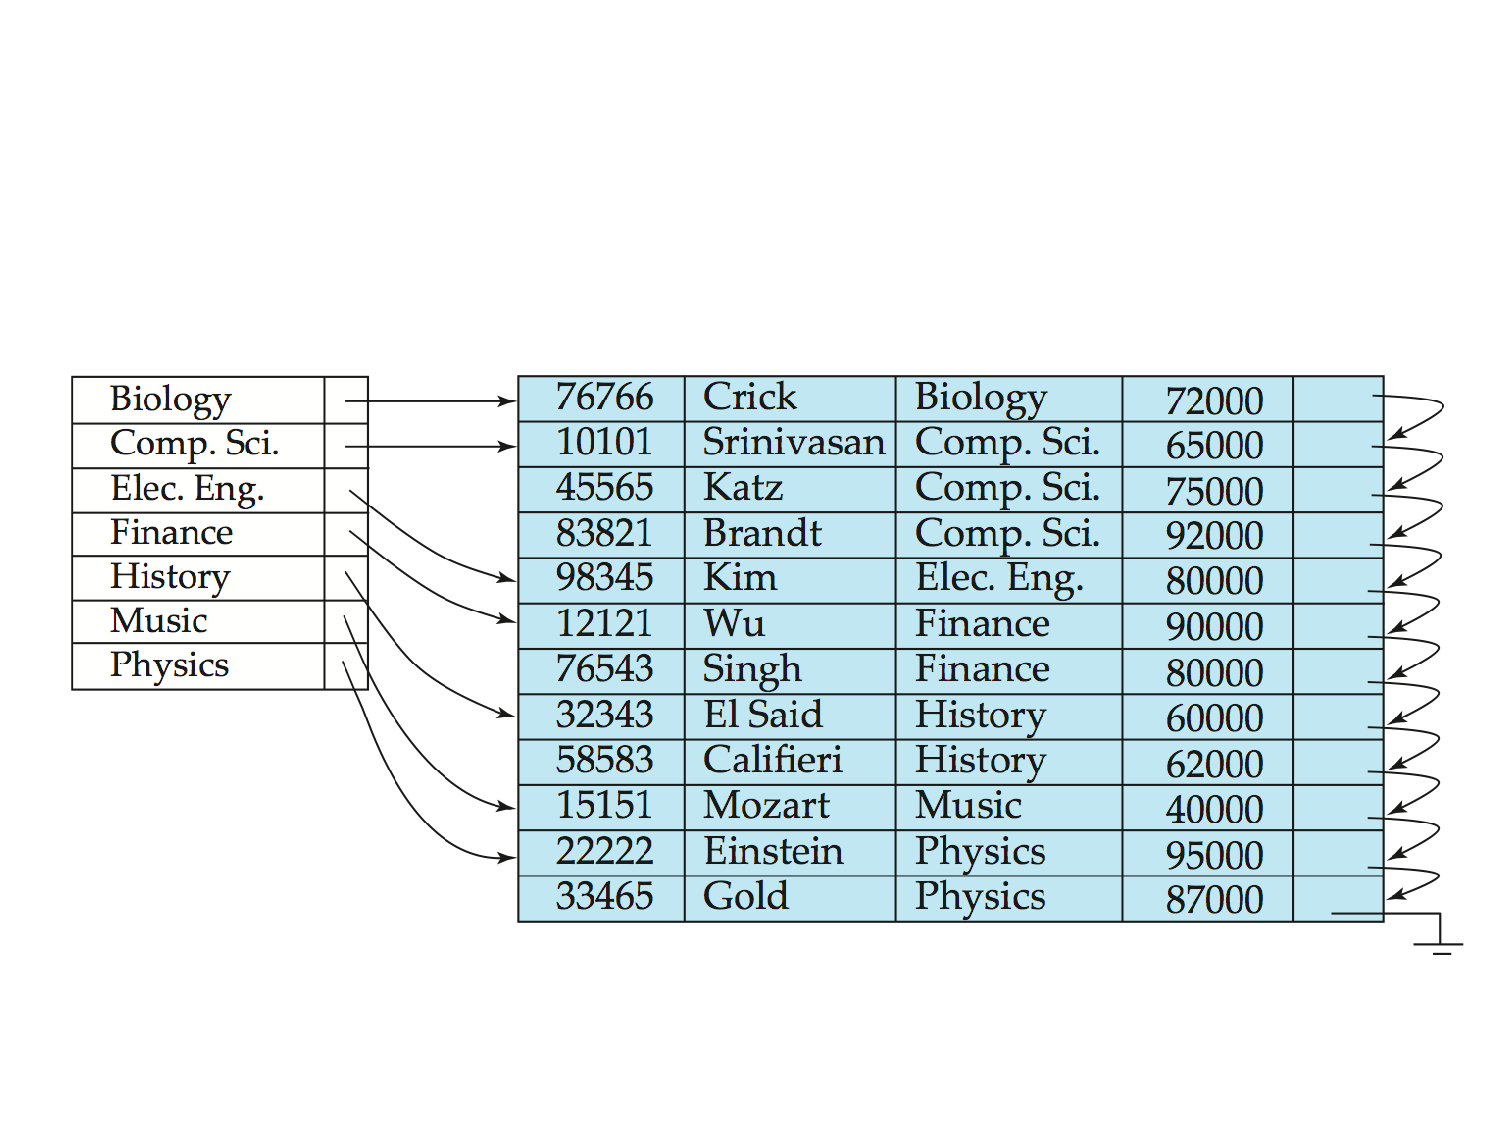
\includegraphics[width=\textwidth]{aula06-denso1}
  \end{minipage}
  %
  \begin{minipage}{0.45\textwidth}
	\centering
	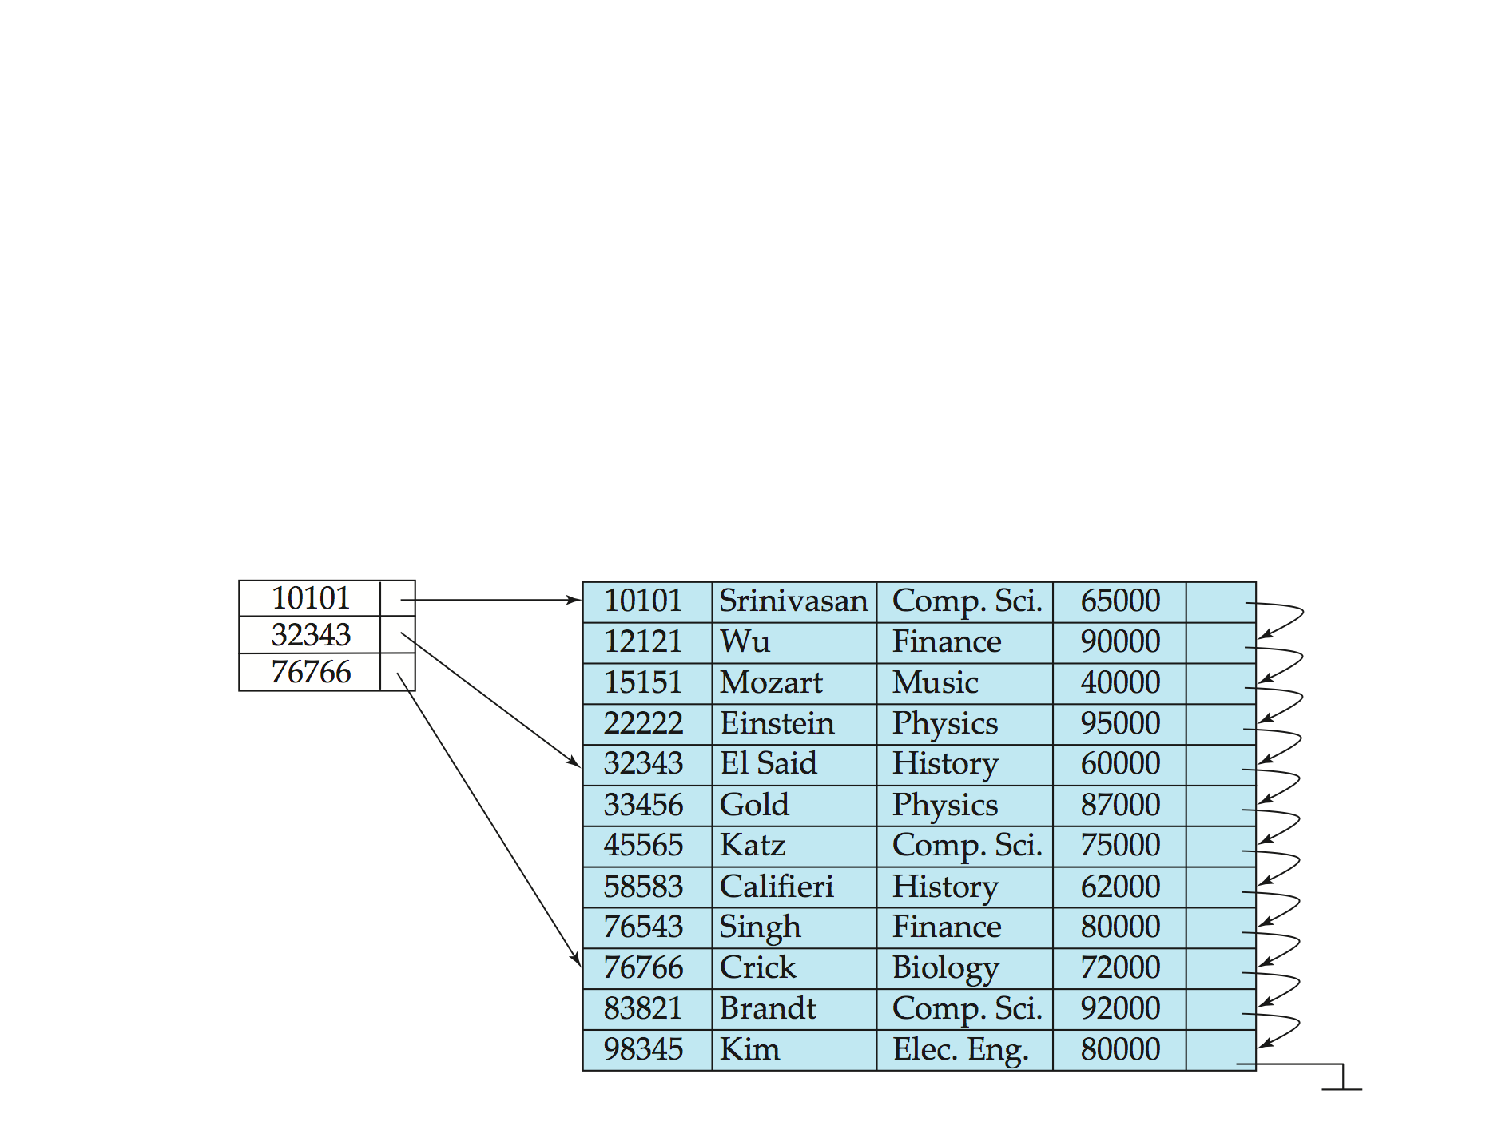
\includegraphics[width=\textwidth]{aula06-esparso1}
  \end{minipage}
\caption{Exemplo de um índice denso (esquerda) e esparso (direita).}
\label{aula06:fig:denso:esparso}
\end{figure}

%%%%%%%%%%%%%%%%%%%%%%%%%%%%%%%%%%%%%%%%%%%%%%%%%%%%%%%%%%%%%%%%%%%%%%%%%%%%%%%
\subsection{Índices multinível}

Para casos em que o índice primário não cabe em memória, o acesso torna-se caro.
Uma solução é tratar o índice primário em disco como um arquivo sequencial e
construir um índice esparso sobre ele.
O \textbf{índice externo} é um índice esparso do índice primário, e 
o \textbf{índice interno} é o arquivo do índice primário.

Se mesmo o índice externo for muito grande para caber na memória, outro nível
pode ser criado, e assim por diante.
Note que índices em todos os níveis devem ser atualizados quando ocorrer
atualizações no arquivo.
A figura~\ref{aula06:fig:multinivel} mostra um simples exemplo de índice esparso
construído de um índice primário.
%
\begin{figure}[!htb]
\centering
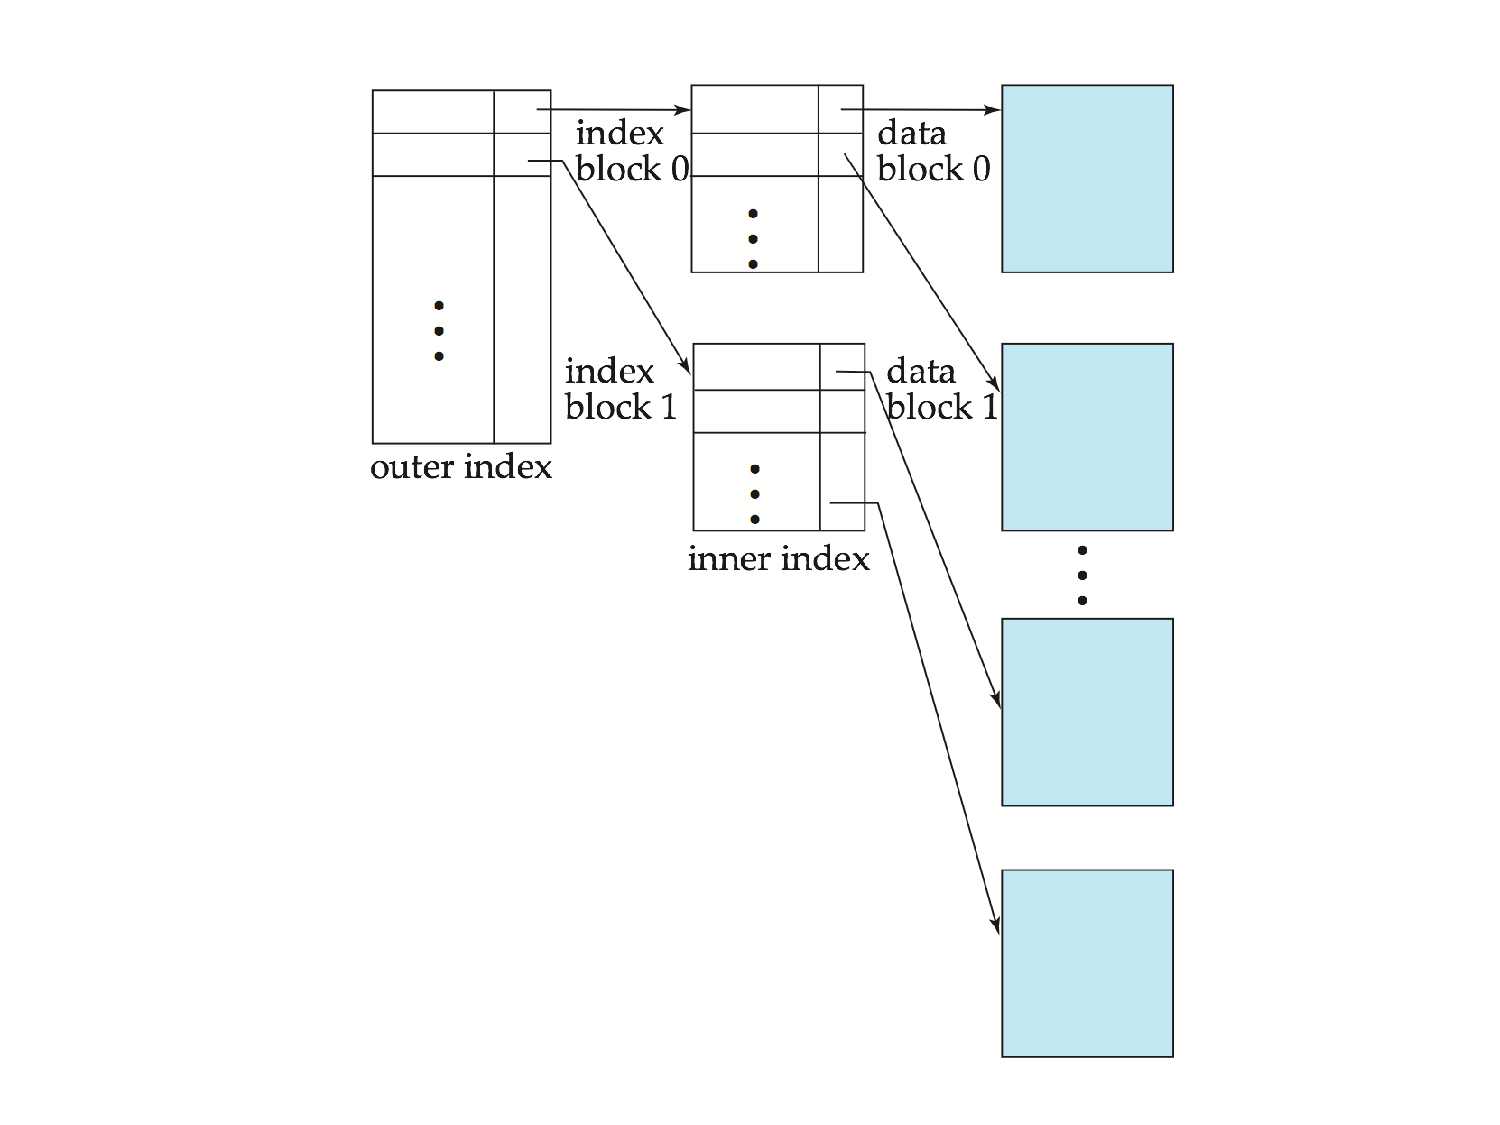
\includegraphics[width=0.4\textwidth]{aula06-multinivel1}
\caption{Índice esparso externo construído de um índice primário.}
\label{aula06:fig:multinivel}
\end{figure}

%%%%%%%%%%%%%%%%%%%%%%%%%%%%%%%%%%%%%%%%%%%%%%%%%%%%%%%%%%%%%%%%%%%%%%%%%%%%%%%
\subsection{Atualização de índice}

Em qualquer das formas de índice, cada índice precisa ser atualizado quando um
registro é inserido ou removido.

{\bf Remoção} - se o registro removido é o único registro no arquivo
com uma chave de busca, a chave de busca também é removida do índice.
Em índices densos, remoção de uma chave de busca é similar a remoção
de um registro de arquivo.
Em índices esparsos, se uma chave de busca existe no índice, ela é removida 
e substituída pela próxima chave de busca do arquivo.
Se a próxima chave de busca já for indexada, a entrada no índice é simplesmente 
removida.

{\bf Inserção} - em índíces densos, realiza uma busca no índice usando a chave de
busca do registro a ser inserido.
Se a chave não existe, ela é inserida no índice.
Em índices esparsos, se o índice mantem uma entrada para cada bloco do arquivo,
nenhuma mudança é necessária, a não ser que um novo bloco seja criado (ou sofra
distribuição).
Se um novo bloco for criado (ou sofrer distribuição), 
a primeira chave de busca nova do bloco é inserida no índice.

Em índices multinível, as inserções e remoções são simples extensões dos
algoritmos usados em índices de um nível só.
As inserções e remoções são propagadas dos níveis internos para os externos.

As atualizações dos índices significam atualizações nos blocos físicos
onde os índices estão armazenados.
A organização física e lógica desses blocos é feita de forma similar
aos blocos de um arquivo de dados.

%%%%%%%%%%%%%%%%%%%%%%%%%%%%%%%%%%%%%%%%%%%%%%%%%%%%%%%%%%%%%%%%%%%%%%%%%%%%%%%
\subsection{Índices secundários}

Em índices secundários, registros do índice apontam para o bucket que contem pointeiros
para todos os registros com uma chave de busca.
A figura~\ref{aula06:fig:secundario} mostra um exemplo de índice secundário.
Note que índices secundários tem de ser densos.
%
\begin{figure}[!htb]
\centering
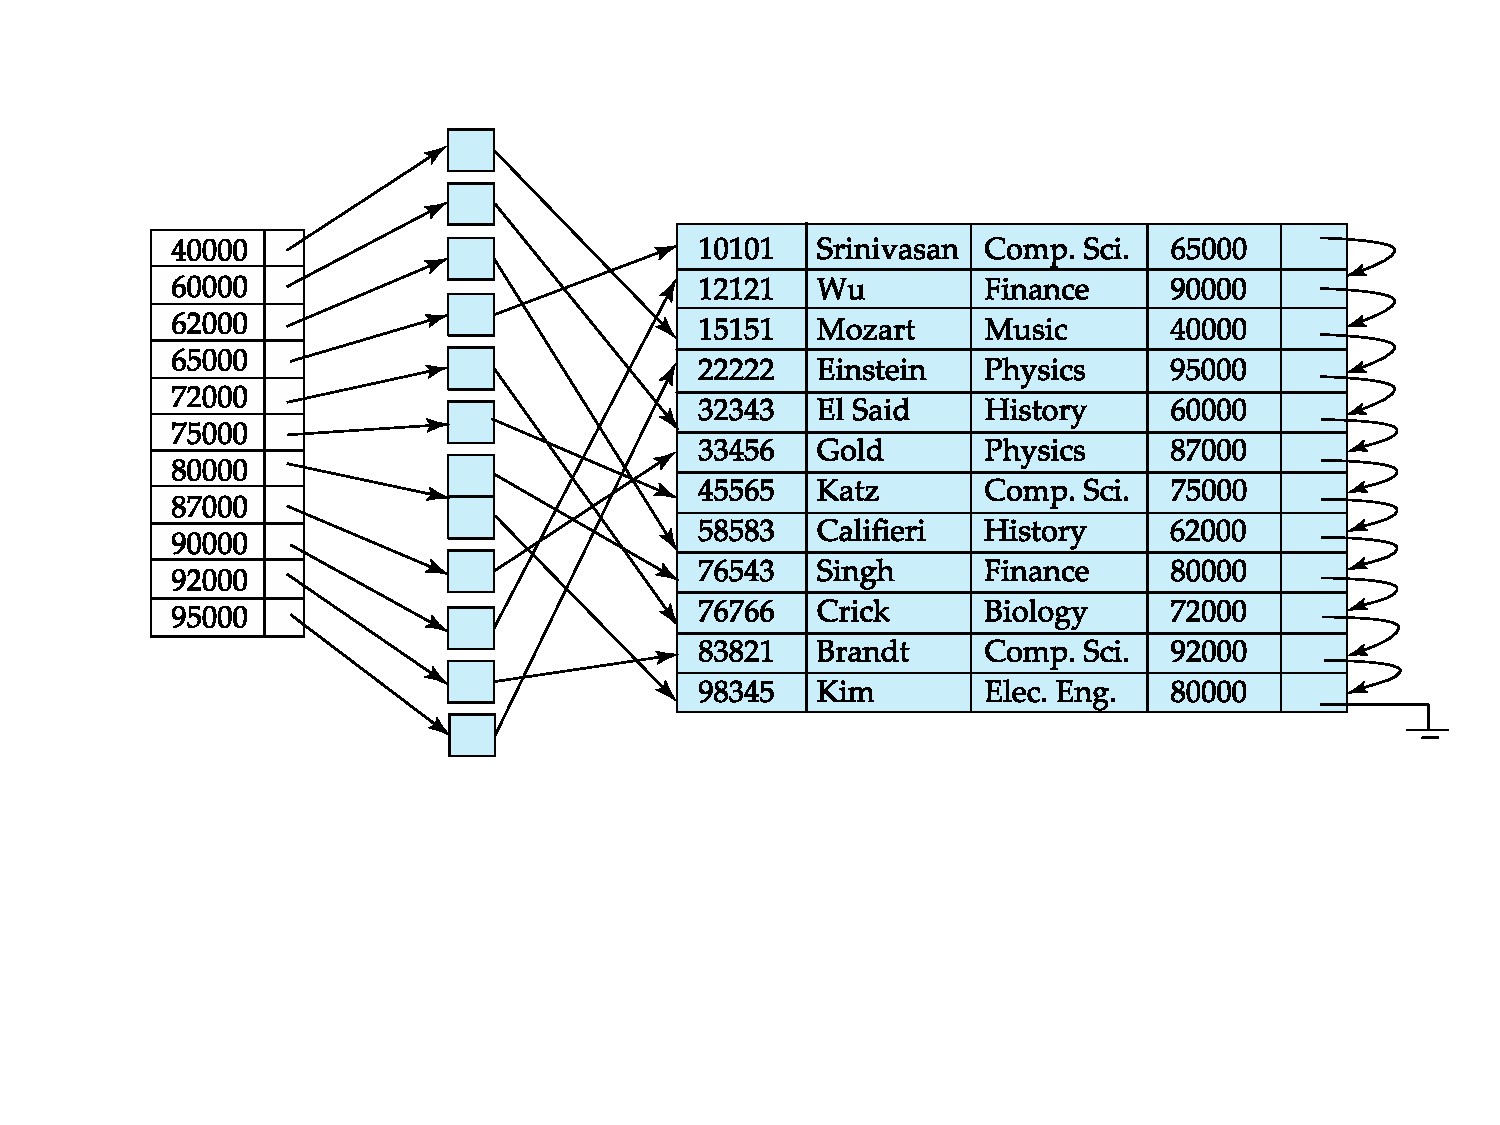
\includegraphics[width=0.6\textwidth]{aula06-secundario1}
\caption{Exemplo de índice secundário sobre o campo \emph{salary}.}
\label{aula06:fig:secundario}
\end{figure}

Índices oferecem benefícios substanciais na busca por registros.
Porém, atualizações de índices impõem sobrecustos em atualizações.

A varredura sequencial de um índice primário é eficiente, mas a 
varredura sequencial em índices secundários é cara pois é preciso
uma transferência de bloco do disco para cada acesso ao registro.
Uma transferência de bloco requer cerca de 5 a 10 milisegundos, contra
100 nanosegundos de um acesso à memória.

%%%%%%%%%%%%%%%%%%%%%%%%%%%%%%%%%%%%%%%%%%%%%%%%%%%%%%%%%%%%%%%%%%%%%%%%%%%%%%%
%\subsection{conceitos basicos}

%%%%%%%%%%%%%%%%%%%%%%%%%%%%%%%%%%%%%%%%%%%%%%%%%%%%%%%%%%%%%%%%%%%%%%%%%%%%%%%
\section{Índices em árvores B+}
%%%%%%%%%%%%%%%%%%%%%%%%%%%%%%%%%%%%%%%%%%%%%%%%%%%%%%%%%%%%%%%%%%%%%%%%%%%%%%%

A principal desvantagem de índices sequenciais é a perda de desempenho
a medida que o arquivo de índice cresce, tanto buscas e varreduras sequenciais.
Reorganizações periódicas são necessárias, mas reorganizações frequentes
são indesejadas.
\textbf{Índices em árvores B+} é um tipo de árvore balanceada que mantem a eficiência
mesmo com inserções e remoções.
Cada nó não-folha de uma árvore B+ tem entre $\lceil n/2 \rceil$ e $n$ filhos,
sendo $n$ fixo para uma árvore particular.

Árvores B+ tem a vantagem de se auto-organizar com modificações pequenas e
locais em inserções e remoções, além de não requerer a reorganização de todo o
arquivo para manter o desempenho.
Uma desvantagem menor é o sobrecusto de inserção e remoção para manter o 
balanceamento, além do sobrecusto em espaço.

A figura~\ref{aula06:fig:btree1} mostra um exemplo de árvore B+.
%
\begin{figure}[!htb]
\centering
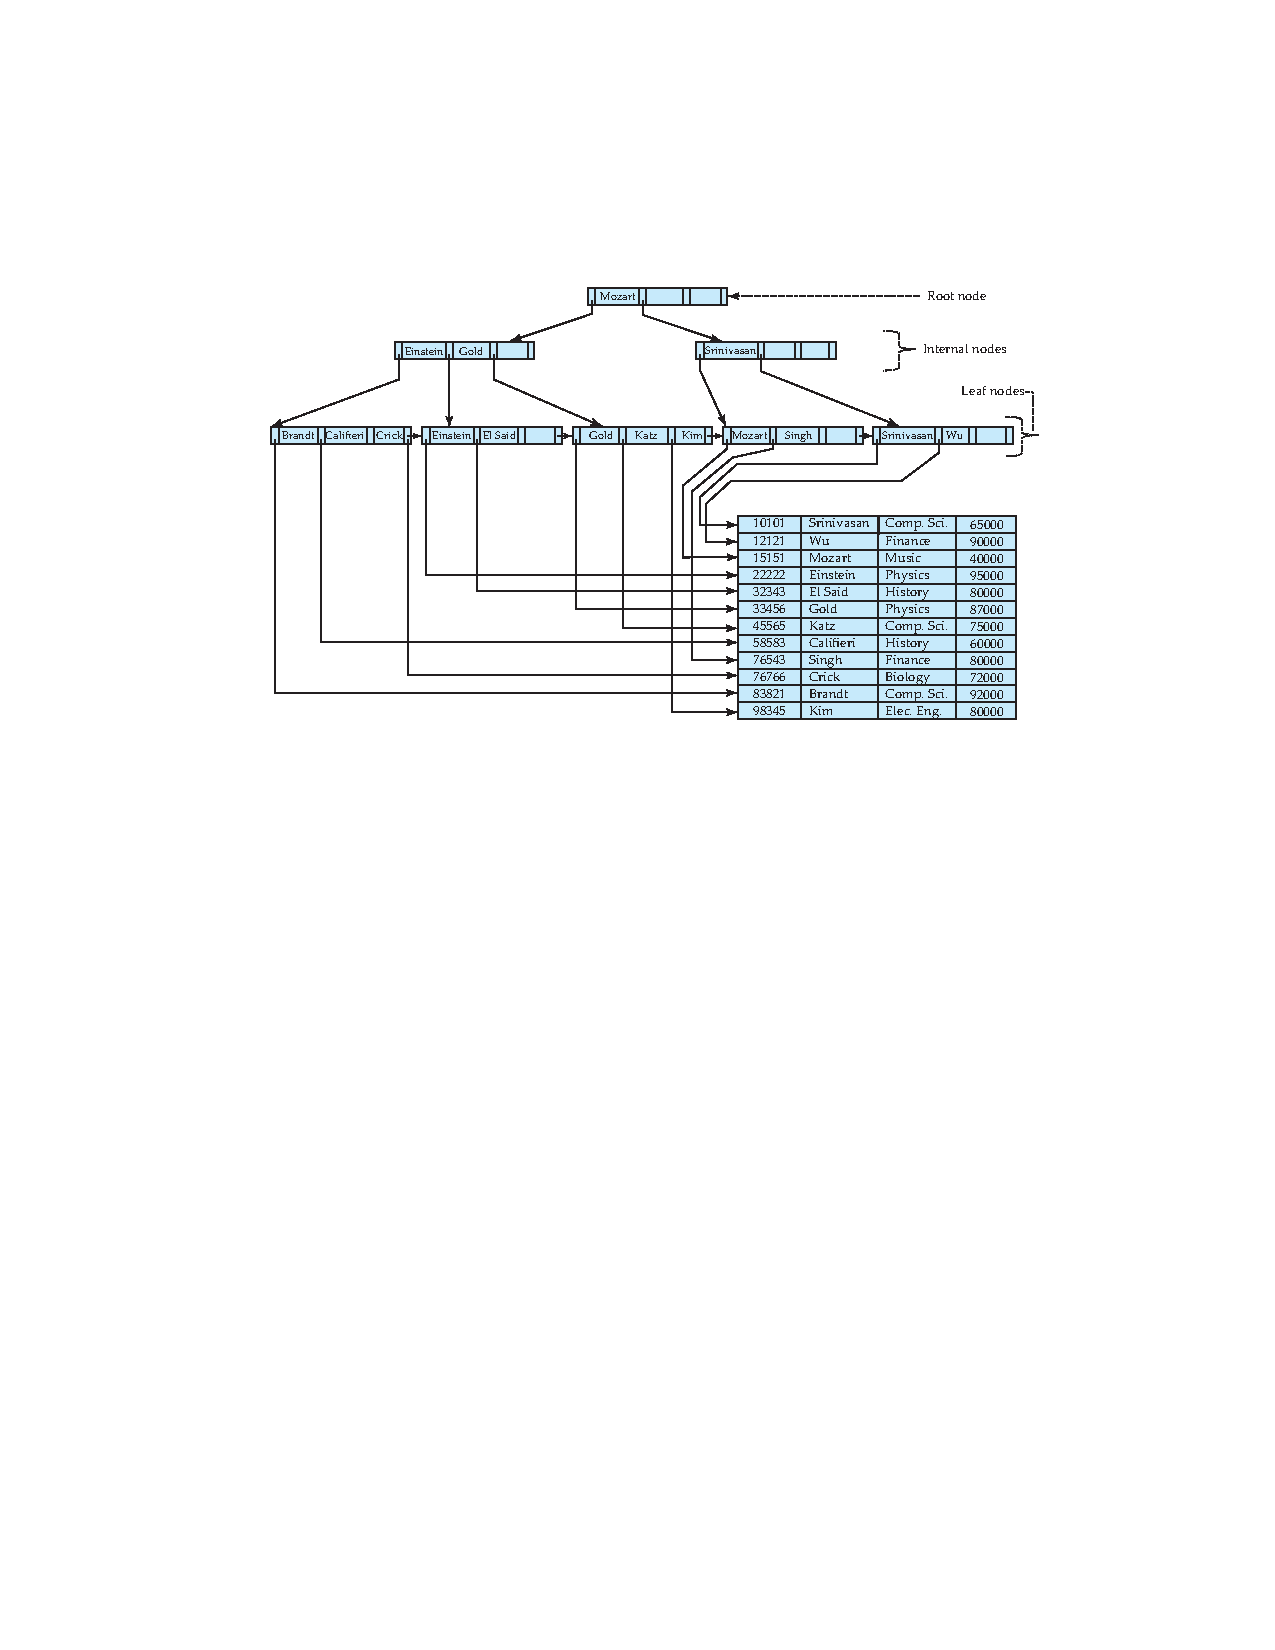
\includegraphics[width=0.7\textwidth]{aula06-btree1}
\caption{Exemplo de uma árvore B+.}
\label{aula06:fig:btree1}
\end{figure}

Uma árvore B+ é uma árvore com raiz única que segue as seguintes propriedades:
\begin{itemize}
\item Todos os caminhos da raiz até as folhas tem o mesmo tamanho.
\item Cada nó que não seja raiz nem folha possui de $\lceil n/2 \rceil$
até $n$ filhos.
\item Um nó folha tem de $\lceil (n-1)/2 \rceil$ até $n-1$ valores.
\item Casos especiais:
	\begin{itemize}
	\item Se a raiz não é uma folha, ela possui pelo menos dois filhos.
	\item Se a raiz é uma folha (ou seja, é o único nó da árvore), ela
	pode ter de $0$ a $(n-1)$ valores.
	\end{itemize}
\end{itemize}

%%%%%%%%%%%%%%%%%%%%%%%%%%%%%%%%%%%%%%%%%%%%%%%%%%%%%%%%%%%%%%%%%%%%%%%%%%%%%%%
\subsection{Estrutura}

Um nó típico de árvore B+, como na figura~\ref{aula06:fig:btree2}, possui:
\begin{itemize}
\item $K_i$ são valores de chaves de busca.
\item $P_i$ são pointeiros para filhos (nós não folha), ou para
registros ou buckets de registros (para nós folha).
\end{itemize}
As chaves de busca de um nó são ordenadas com $K_1 < K_2 < K_3 < ... < K_{n-1}$.
Normalmente o nó tem o tamanho de um bloco.
%
\begin{figure}[!htb]
\centering
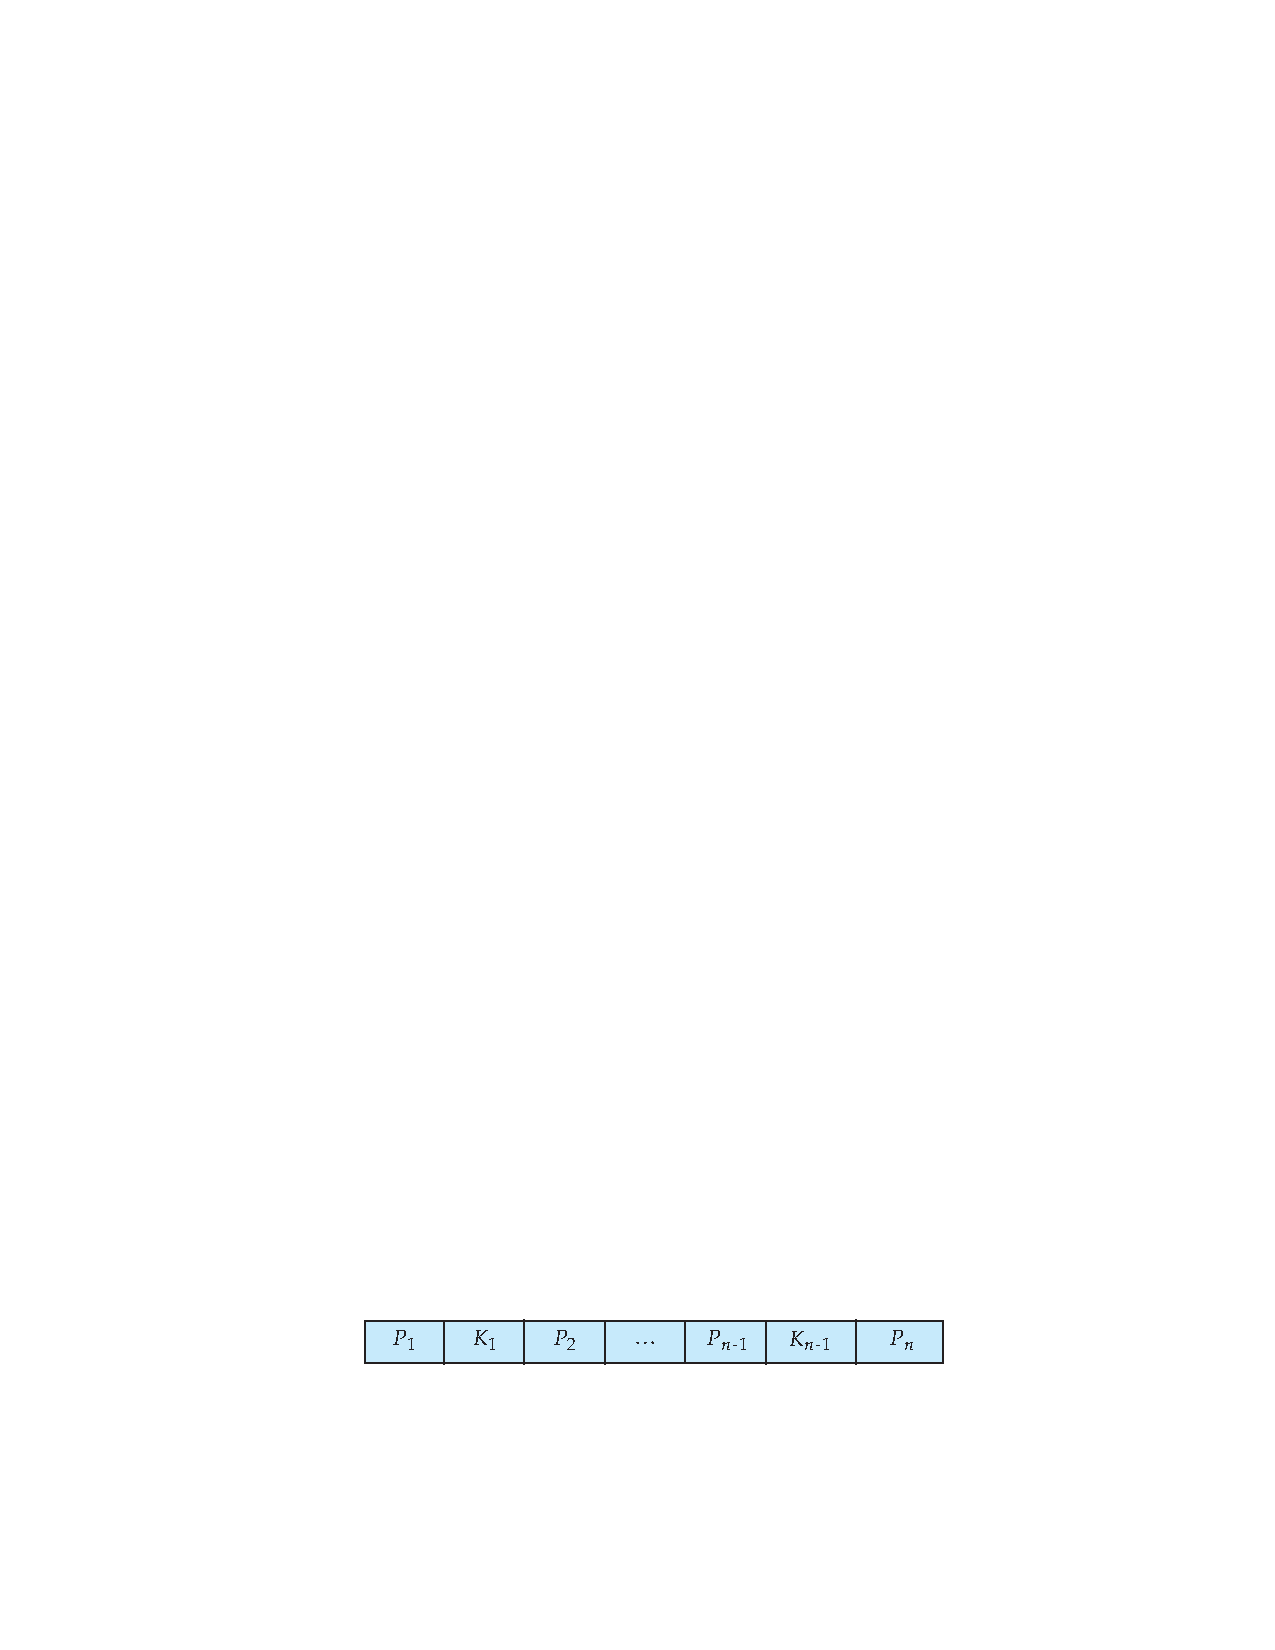
\includegraphics[width=0.4\textwidth]{aula06-btree2}
\caption{Um nó em uma árvore B+.}
\label{aula06:fig:btree2}
\end{figure}

As propriedades de um nó folha, como na figura~\ref{aula06:fig:btree3}, são:
\begin{itemize}
\item Para $i = 1, 2, ..., n-1$, o ponteiro $P_i$ aponta
para o registro com chave de busca $K_i$, ou para um bucket de apontadores para registros.
Buckets só são necessários se a chave de busca não for chave primária.
\item Se $L_i$, $L_j$ são nós folha e $i < j$, as chaves de busca de $L_i$
são menores que as chaves de busca de $L_j$.
\item $P_n$ aponta para o próximo nó folha na ordem da chave de busca.
\end{itemize}
%
\begin{figure}[!htb]
\centering
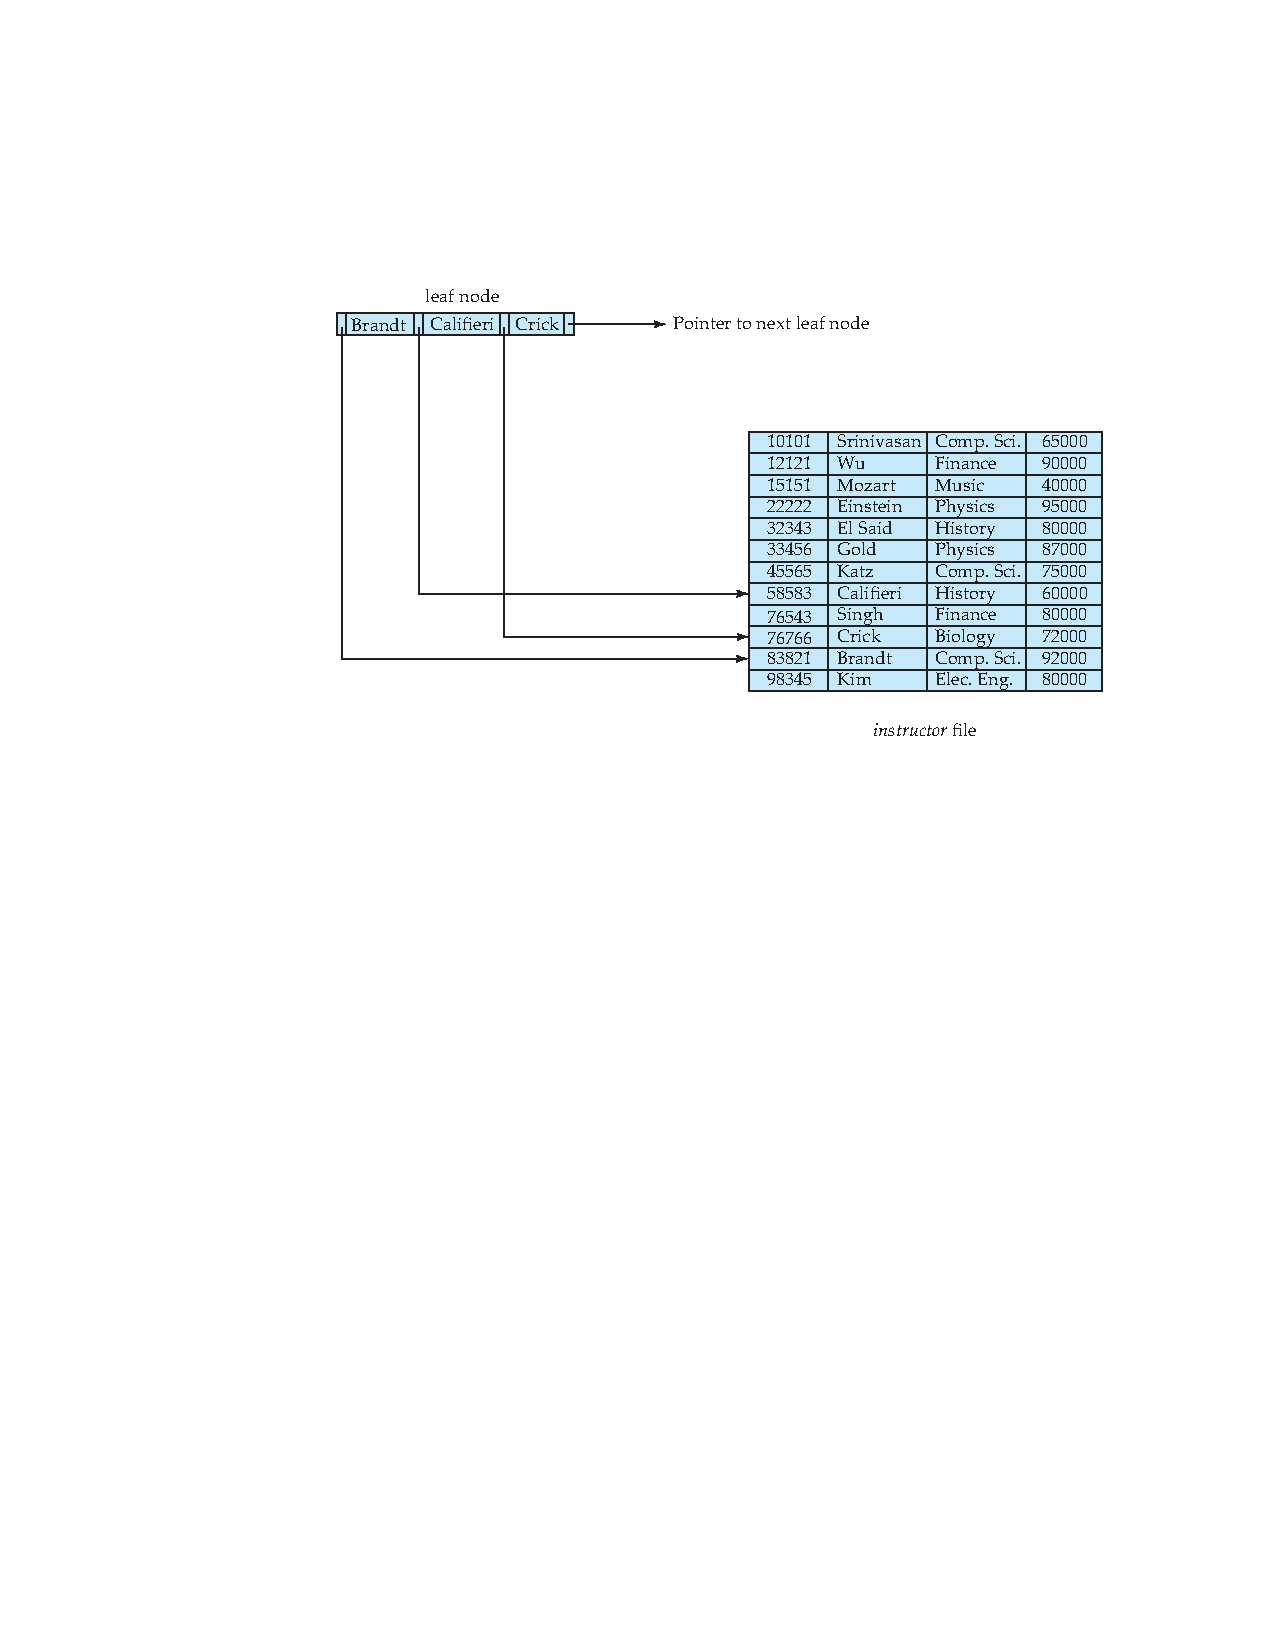
\includegraphics[width=0.6\textwidth]{aula06-btree3}
\caption{Exemplo de um nó folha ($n = 4$) de uma árvore B+.}
\label{aula06:fig:btree3}
\end{figure}

Ao passo que nós não folha formam um índice esparso multinível sobre os nós folha.
Para um nó não folha, como na figura~\ref{aula06:fig:btree2}, com $m$ ponteiros:
\begin{itemize}
\item Todas as chaves de busca da subárvore apontada por $P_1$ são 
menores do que $K_1$.
\item Para $2 \leq i \leq n-1$, todas as chaves de busca da sub-árvore apontada
por $P_i$ são maiores ou iguais a $K_{i-1}$ e menores que $K_i$.
\item Todas as chaves de busca da sub-árvore apontada por $P_n$ são maiores
ou iguais a $K_{n-1}$.
\end{itemize}

A figura~\ref{aula06:fig:btree4} ilustra um exemplo de árvore B+ com $n = 6$.
Baseado nessa figura, podemos afirmar que:
\begin{itemize}
\item Nós folha tem de 3 a 5 valores ($\lceil (n-1)/2 \rceil$ e $n-1$, com $n=6$).
\item Nós não folha (que não a raiz) tem de 3 a 6 filhos ($\lceil n/2 \rceil$ e
$n$ com $n=6$).
\item A raiz precisa ter pelo menos $2$ filhos.
\end{itemize}
%
\begin{figure}[!htb]
\centering
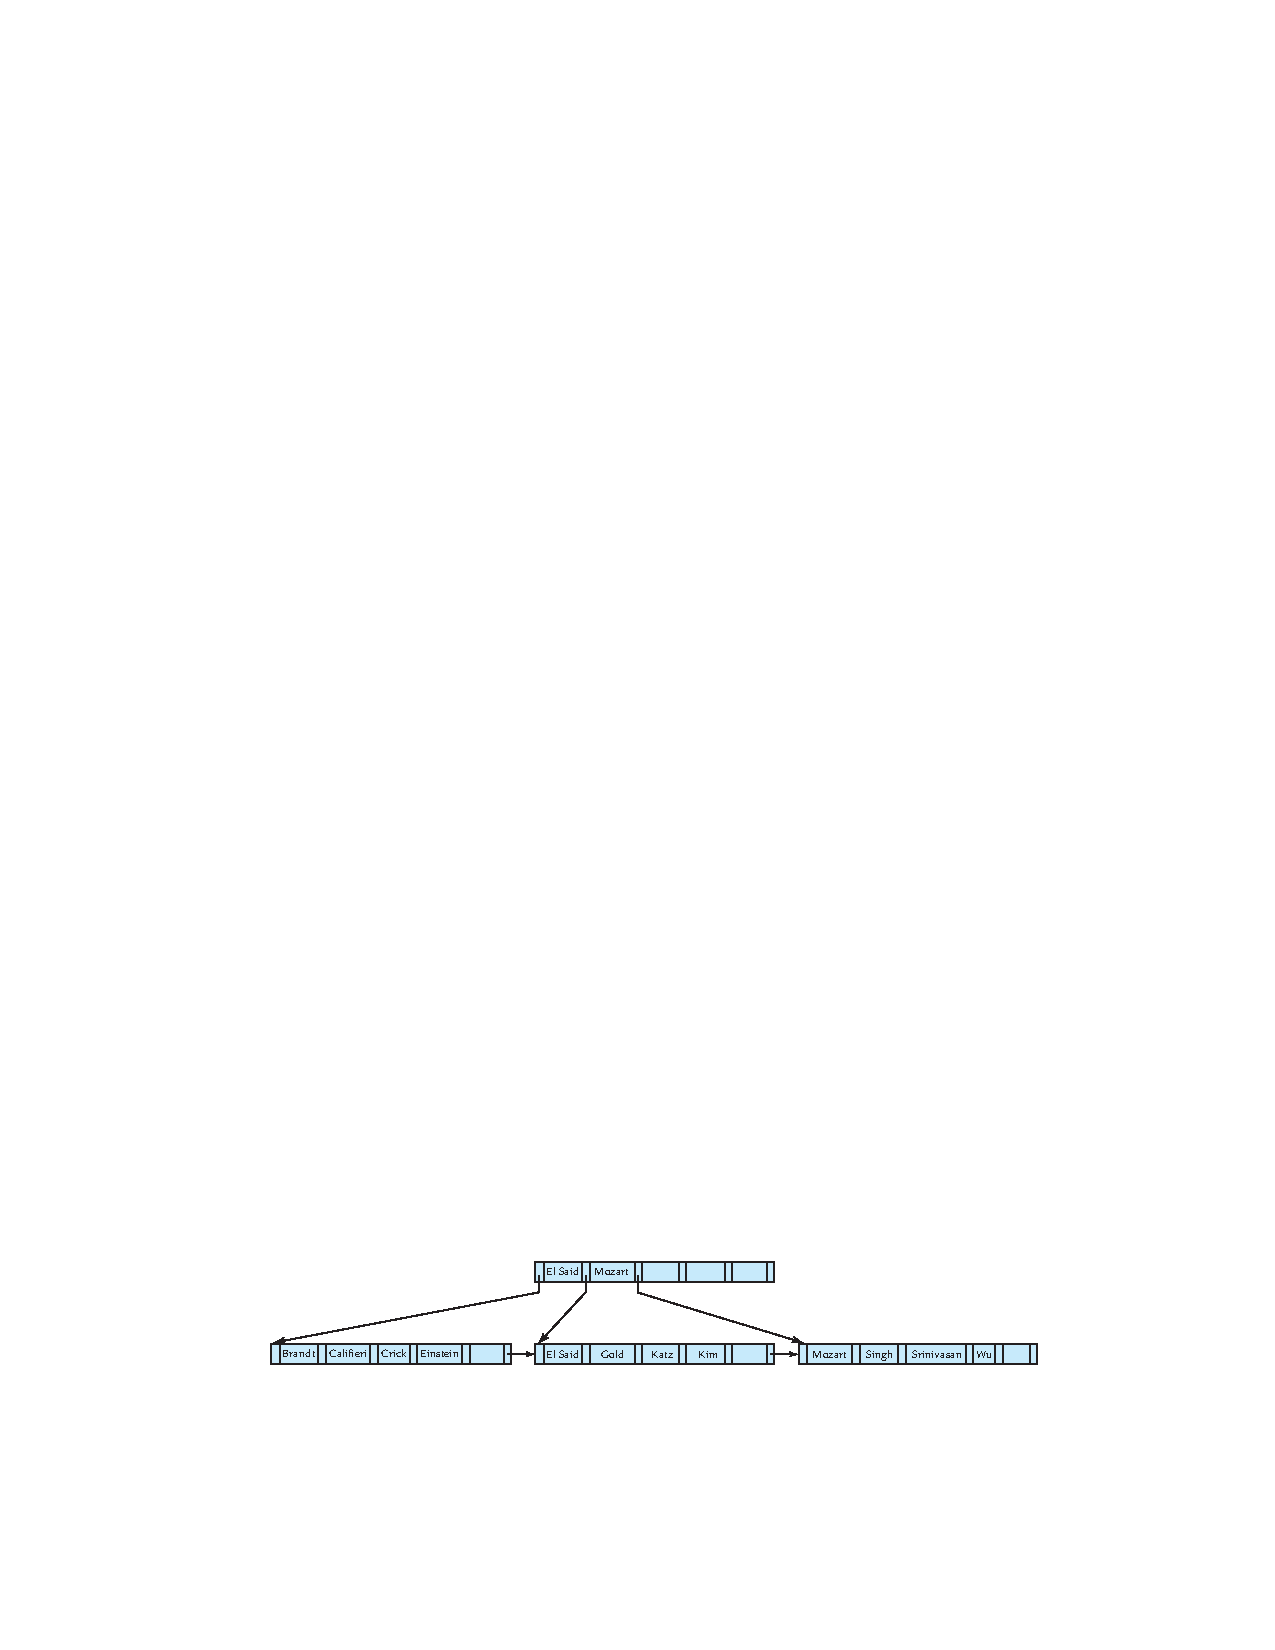
\includegraphics[width=0.8\textwidth]{aula06-btree4}
\caption{Árvore B+ com $n = 6$.}
\label{aula06:fig:btree4}
\end{figure}

Algums observações sobre árvores B+:
\begin{itemize}
\item Visto que as conexões entre nós são feitas por ponteiros, 
blocos ``logicamente'' próximos não precisam estar ``fisicamente'' 
próximos.

\item Os níveis não folha de uma árvore B+ formam uma hierarquia 
multinível de índices esparsos.

\item A árvore possui um número relativamente pequeno de níveis:
	\begin{itemize}
	\item O nível abaixo da raiz possui pelo menos $2 * \lceil n/2 \rceil$ valores.
	\item O próximo nível possui pelo menos $2 * \lceil n/2 \rceil * \lceil n/2 \rceil$ valores.
	\item ... etc.
	\item Se existem $K$ chaves de busca, a altura não é maior do que $\lceil \log_{n/2} K \rceil$.
	\item Por isso as buscas são eficientes.
	\end{itemize}
\item Inserções e remoções são eficientes, já que o índice é reestruturado em tempo 
logarítimico, como será visto adiante.
\end{itemize}

%%%%%%%%%%%%%%%%%%%%%%%%%%%%%%%%%%%%%%%%%%%%%%%%%%%%%%%%%%%%%%%%%%%%%%%%%%%%%%%
\subsection{Busca}

Os passos na busca em árvores B+ para uma chave de busca de valor $V$
onde retorna $C$ e o índice $i$ tal que $C.P_i$ aponta para o primeiro registro
com chave de busca $V$:
\begin{enumerate}
\item C = raiz.
\item \textbf{Repete} enquanto $C$ não é um nó folha:
	\begin{enumerate}
	\item Seja $i= $ o menor número tal que $V \leq C.K_i$.
	\item \textbf{Se} não existir um $i$, então $C = C.P_m$ onde $P_m$ é o último ponteiro não-nulo do nó.
	\item \textbf{Senão} (existe um $i$):
		\begin{enumerate}
		\item \textbf{Se} $V = C.K_i$, então $C = C.P_{i+1}$.
		\item \textbf{Senão} $C = C.P_i$ ($V < C.K_i$).
		\end{enumerate}
	\end{enumerate}
\item Seja $i$ o valor mínimo tal que $K_i = V$.
\item \textbf{Se} existe um $i$, retorna $(C, i)$, \textbf{senão} retorna $null$.
\end{enumerate}

Se o arquivo de índice possui $K$ chaves de busca, a altura da árvore não
ultrapassa $\lceil \log_{\lceil n/2 \rceil} K \rceil$
Um nó é geralmente do mesmo tamanho de um bloco, tipicamente $4$ Kbytes, e 
$n$ é tipicamente cerca de 100 (40 bytes por entrada no índice).
Com 1 milhão de chaves de busca e $n= 100$, no máximo $\log_{50}(1,000,000) = 4$
nós são acessados em uma busca, ou seja, no máximo 4 acessos a blocos.
Compare isso com uma árvore binária balanceada com 1 milhão de chaves de busca,
que acessa cerca de 20 nós em uma busca.
A diferença é significativa já que cada acesso a nó requer um acesso a disco.

%%%%%%%%%%%%%%%%%%%%%%%%%%%%%%%%%%%%%%%%%%%%%%%%%%%%%%%%%%%%%%%%%%%%%%%%%%%%%%%
\subsection{Atualização}

\subsubsection{Inserção}

Os passos para inserção em uma árvore B+ são:
\begin{enumerate}
\item Encontre o nó folha onde a chave de busca deveria aparecer.
\item Se a chave existir no nó folha:
	\begin{enumerate}
	\item Adicionar registro no arquivo.
	\item Adicionar o ponteiro no bucket.
	\end{enumerate}
\item Se a chave de busca não estiver presente:
	\begin{enumerate}
	\item Adicionar o registro no arquivo e criar o bucket.
	\item Se tiver espaço no nó folha, inserir par (chave, pointeiro).
	\item Senão, dividir o nó folha, junto com o novo par (chave-valor).
	\end{enumerate}
\end{enumerate}

A divisão do nó folha envolve os seguintes passos:
\begin{enumerate}
\item Pegar os $n$ pares (chave, apontador) (incluindo o novo) em ordem. Colocar os primeiros $\lceil n/2 \rceil$ no nó original e o restante no novo nó.
\item Considere que o novo nó é $p$, e $k$ é a menor chave em $p$. 
Inserir $(k,p)$ no pai do nó sendo dividido.
\item Se o pai estiver cheio, divida-o e propague a divisão para cima. A divisão prossegue até que se encontre um nó não cheio.
\end{enumerate}
%
Um exemplo de inserção é mostrado na figura~\ref{aula06:fig:btree6}.
%
\begin{figure}[!htb]
\centering
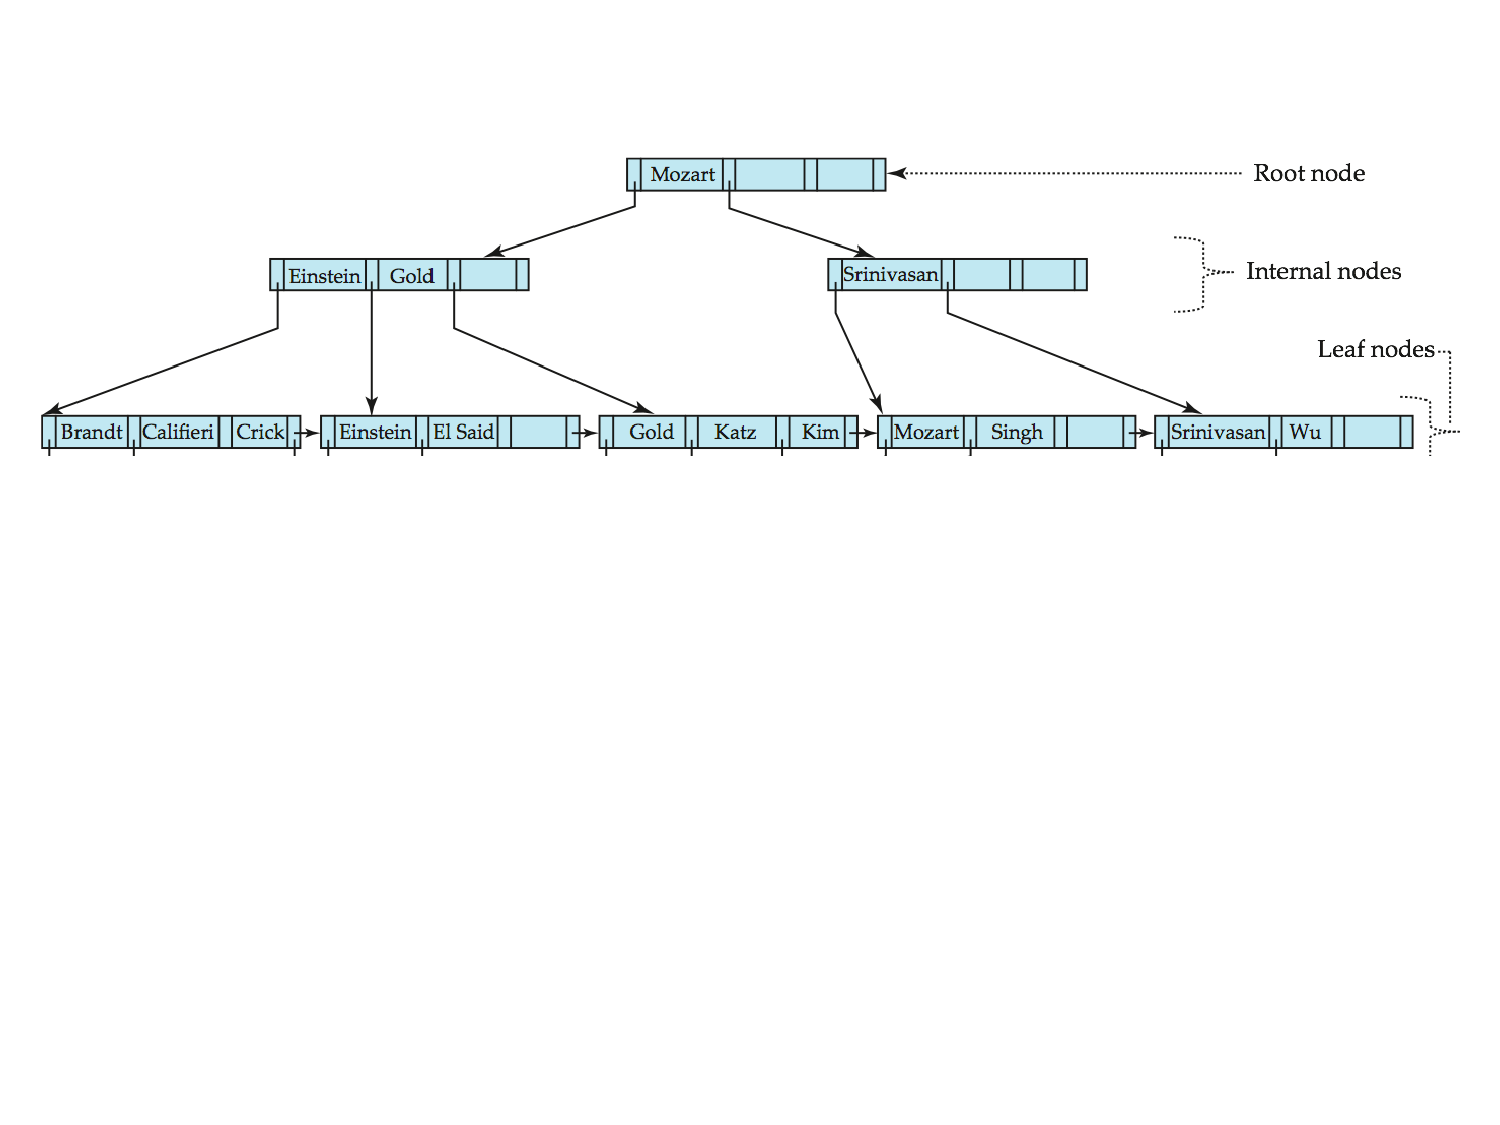
\includegraphics[width=0.8\textwidth]{aula06-btree6}
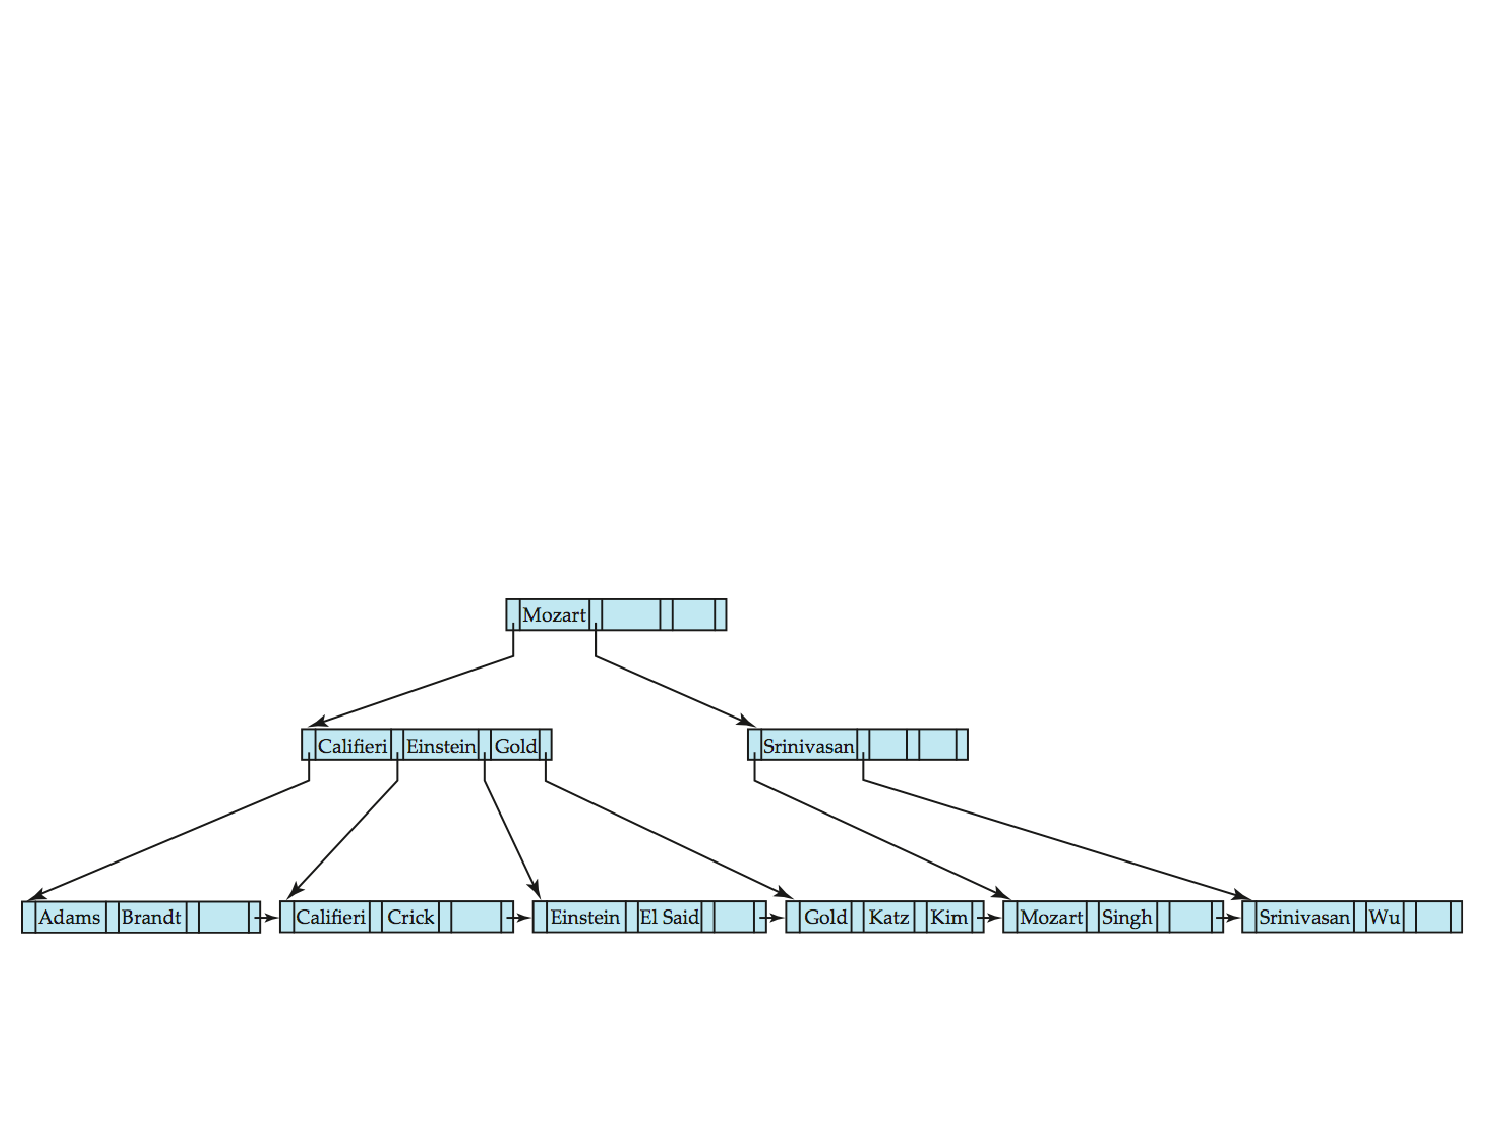
\includegraphics[width=0.8\textwidth]{aula06-btree7}
\caption{Árvore B+ antes e depois da inserção de ``Adams''.}
\label{aula06:fig:btree6}
\end{figure}

No pior caso, a raiz será dividida, aumentando a altura da árvore em uma
unidade.

Os passos na divisão de um nó não folha, quando ao inserir $(k,p)$
em um nó interno $N$ já cheio, são:
\begin{enumerate}
\item Copiar $N$ para uma área temporária $M$ com espaço para $n+1$ pointeiros
e $n$ chaves.
\item Inserir $(k,p)$ em $M$.
\item Copiar $P_1,K_1, ..., K_{\lceil n/2 \rceil -1}, P_{\lceil n/2 \rceil}$ de
$M$ para o nó $N$. 
\item Copiar $P_{\lceil n/2 \rceil + 1}, K_{\lceil n/2 \rceil+1}, ..., K_n,
P_{n+1}$ de $M$ para o novo nó $N'$.
\item Inserir $(K_{\lceil n/2 \rceil},N')$ no pai $N$.
\end{enumerate}
A figura~\ref{aula06:fig:btree5} mostra um exemplo da divisão de um nó
não-folha cheio e inserção do no pai $N$.
%
\begin{figure}[!htb]
\centering
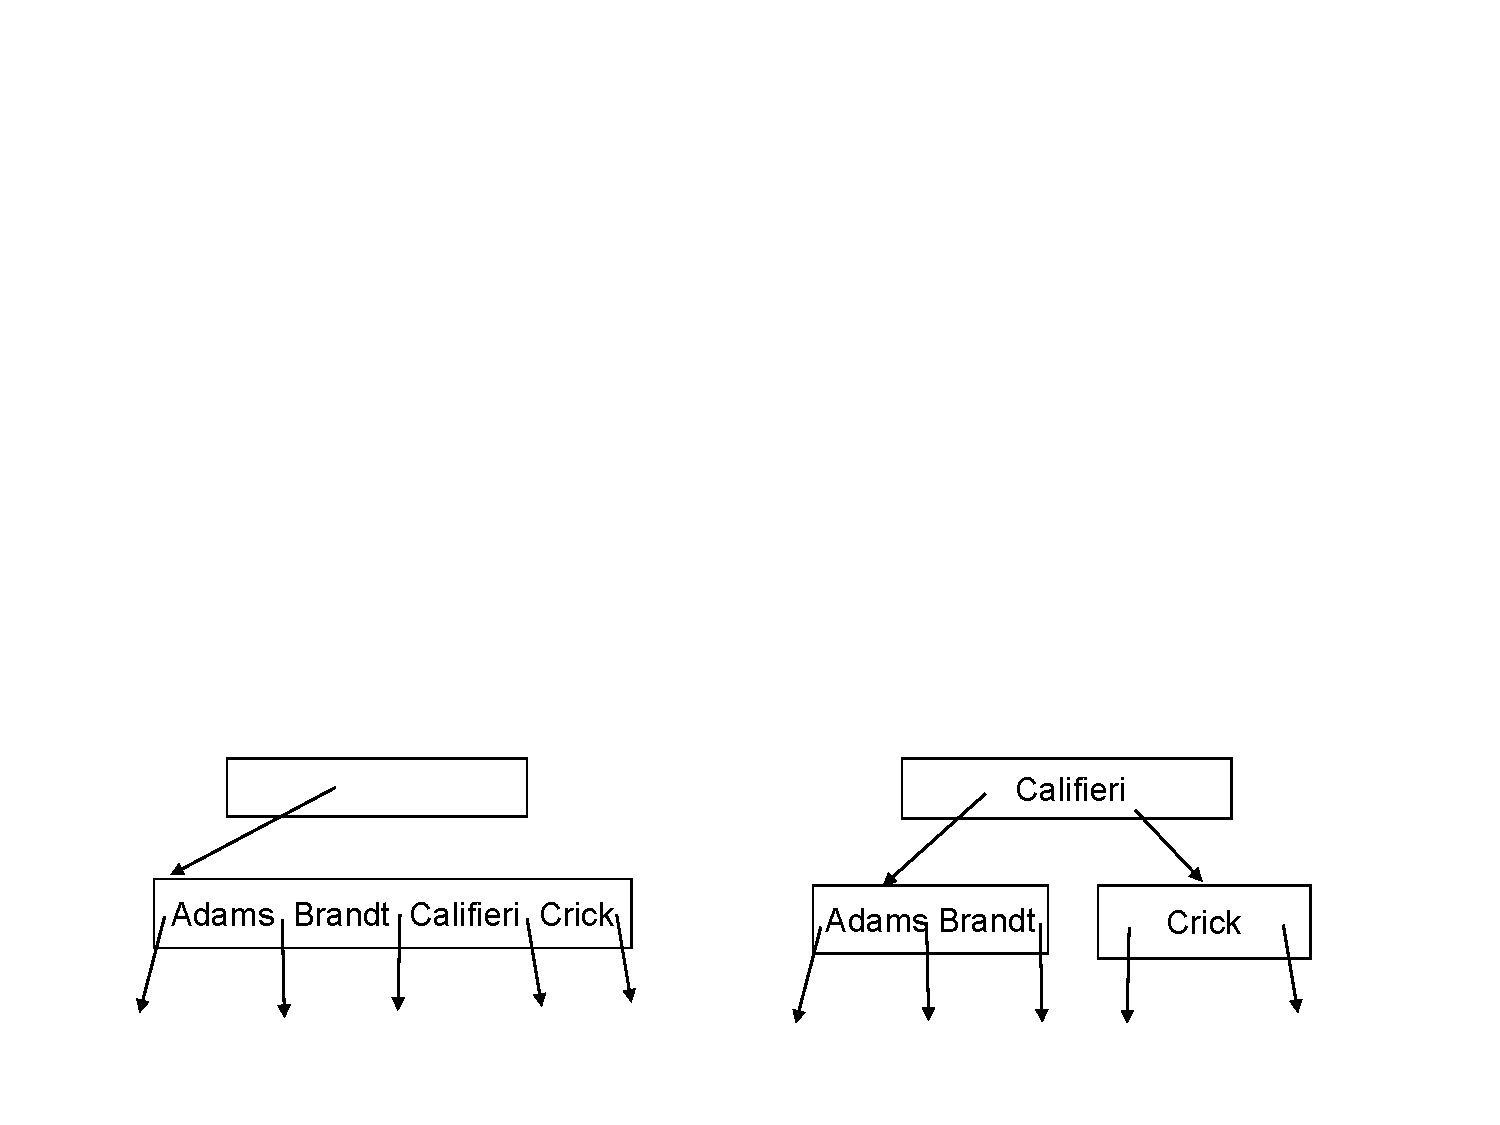
\includegraphics[width=0.7\textwidth]{aula06-btree5}
\caption{Exemplo de uma divisão de nó não-folha cheio.}
\label{aula06:fig:btree5}
\end{figure}

\subsubsection{Remoção}

Os passos da remoção são:
\begin{enumerate}
\item Encontrar os registros a serem removidos, removê-los do
arquivo e do bucket (se necessário).
\item Remover (chave, pointeiro) do nó folha se não tiver bucket ou se 
o bucket estiver vazio.
\item Se o nó possuir poucas entradas devido a remoção, e as entradas 
do nó e seu vizinho couberem no mesmo nó, então \textbf{mesclar vizinhos}:
	\begin{enumerate}
	\item Inserir todas as chaves dos dois nós em um só (o da esquerda) e 
	remover o outro.
	\item Remover o pai do par $(K_{i-1}, P_i)$, onde $P_i$ é o ponteiro
	para o nó removido.
	\item Repetir o procedimento se o pai ficar com poucas entradas.
	\end{enumerate}
\item Senão, se o nó possuir poucas entradas, mas as entradas no nó
e no vizinho não couberem em um só, então \textbf{redistribuir ponteiros}:
	\begin{enumerate}
	\item Redistribuir os ponteiros entre o nó e o vizinho de modo
	que ambos tenham mais do que o número mínimo de entradas.
	\item Atualizar as chaves correspondentes do nó pai.
	\end{enumerate}
\end{enumerate}

As remoções podem se propagar para cima até que se encontre um nó com pelo 
menos $\lceil n/2 \rceil$ pointeiros.
Se o nó raiz possuir apenas um ponteiro após a remoção, ele é removido e seu filho
se torna a raiz.
A figura~\ref{aula06:fig:btree8} mostram o exemplo de remoção.
%
\begin{figure}[!htb]
\centering
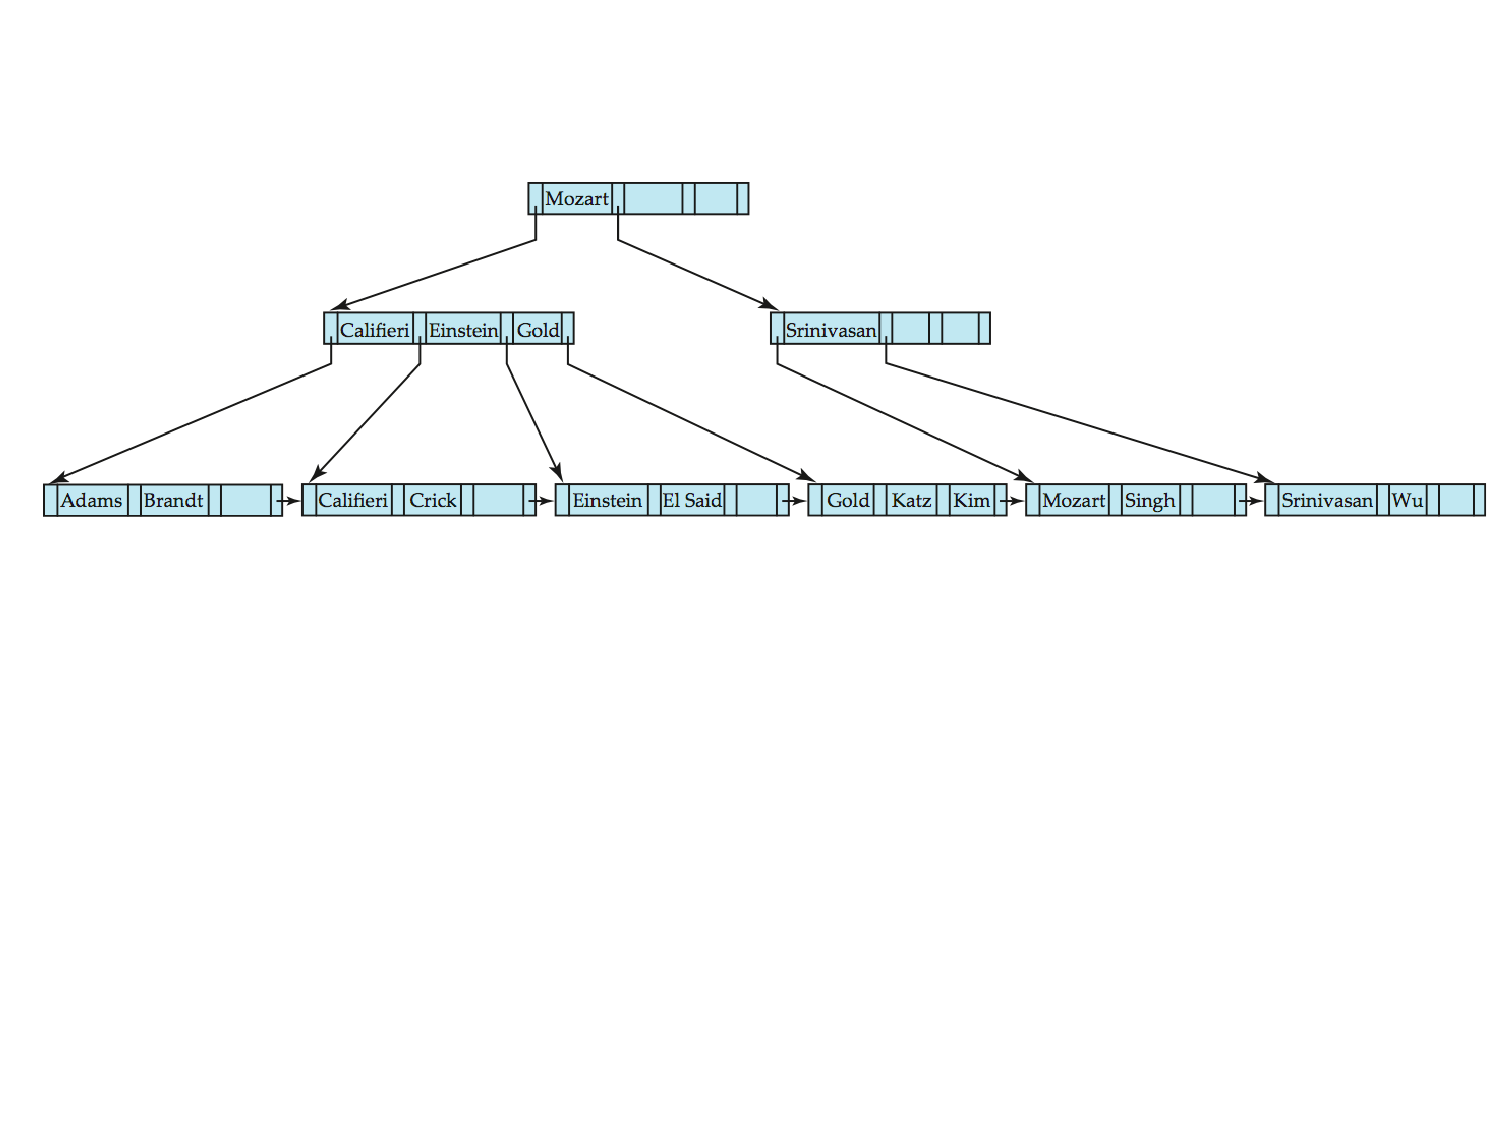
\includegraphics[width=0.8\textwidth]{aula06-btree8}
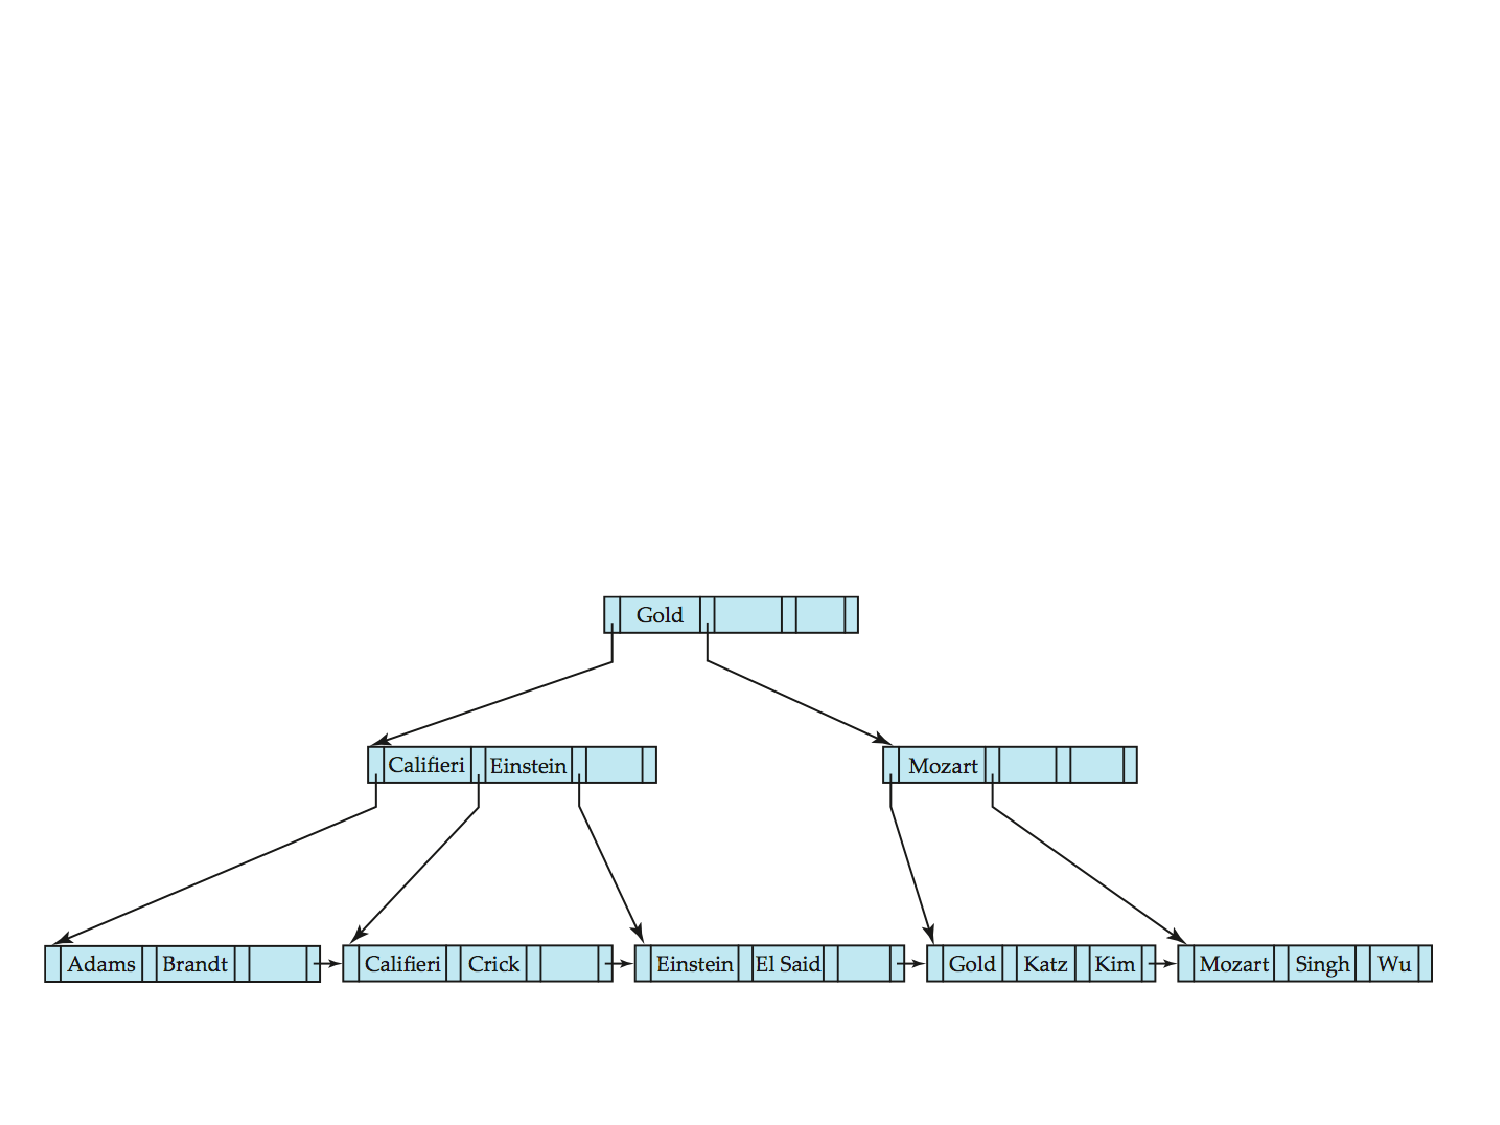
\includegraphics[width=0.8\textwidth]{aula06-btree9}
\caption{Árvore B+ antes e depois da remoção de ``Srinivasan''.}
\label{aula06:fig:btree8}
\end{figure}

%%%%%%%%%%%%%%%%%%%%%%%%%%%%%%%%%%%%%%%%%%%%%%%%%%%%%%%%%%%%%%%%%%%%%%%%%%%%%%%
\subsection{Organização de arquivos}

Árvores B+ podem ser usadas diretamente para organizar arquivos
em vez de simplesmente para indexação. 
Nesse caso, os nós folhas armazenam registros em vez de ponteiros.
O problema da degradação de arquivo é resolvida usando essa solução.
A inserção e remoção são tratadas da mesma forma.

As folhas ainda precisam estar preenchidas até a metade visto
registros são mais longos do que pointeiros, 
o máximo de registros em um nó folha é menor do que o número de ponteiros
dos nós não-folha.

Para melhorar a utilização de espaço, pode-ser envolver mais vizinhos na 
redistribuição durante as divisões e mesclas.
Por exemplo, usar 2 vizinhos na redistribuição (para evitar divisões/mesclas)
resulta em cada nó tendo pelo menos $\lfloor 2n/3 \rfloor$ entradas.

%%%%%%%%%%%%%%%%%%%%%%%%%%%%%%%%%%%%%%%%%%%%%%%%%%%%%%%%%%%%%%%%%%%%%%%%%%%%%%%
\section{Índices Hash}
%%%%%%%%%%%%%%%%%%%%%%%%%%%%%%%%%%%%%%%%%%%%%%%%%%%%%%%%%%%%%%%%%%%%%%%%%%%%%%%

%%%%%%%%%%%%%%%%%%%%%%%%%%%%%%%%%%%%%%%%%%%%%%%%%%%%%%%%%%%%%%%%%%%%%%%%%%%%%%%
\subsection{Hashing estático}

Por definição, um \textbf{bucket} é uma unidade de armazenamento com um ou mais
registros. Tipicamente, um bucket pode ser um bloco de disco.
Em uma organização de arquivo com hash, o bucket de um registro é obtido diretamente
de sua chave de busca por meio da \textbf{função hash}.

Uma função hash mapeia todas as chaves de busca para buckets, e é usada
para localizar registros para acesso, inserção e remoção.
Registros com valores de chave de busca diferentes podem ser mapeados para o mesmo
bucket.
Para localizar um registro, todo o bucket deve ser varrido sequencialmente.

A figura~\ref{aula06:fig:hash1} mostram o exemplo de arquivo hash com hashing estático.
%
\begin{figure}[!htb]
\centering
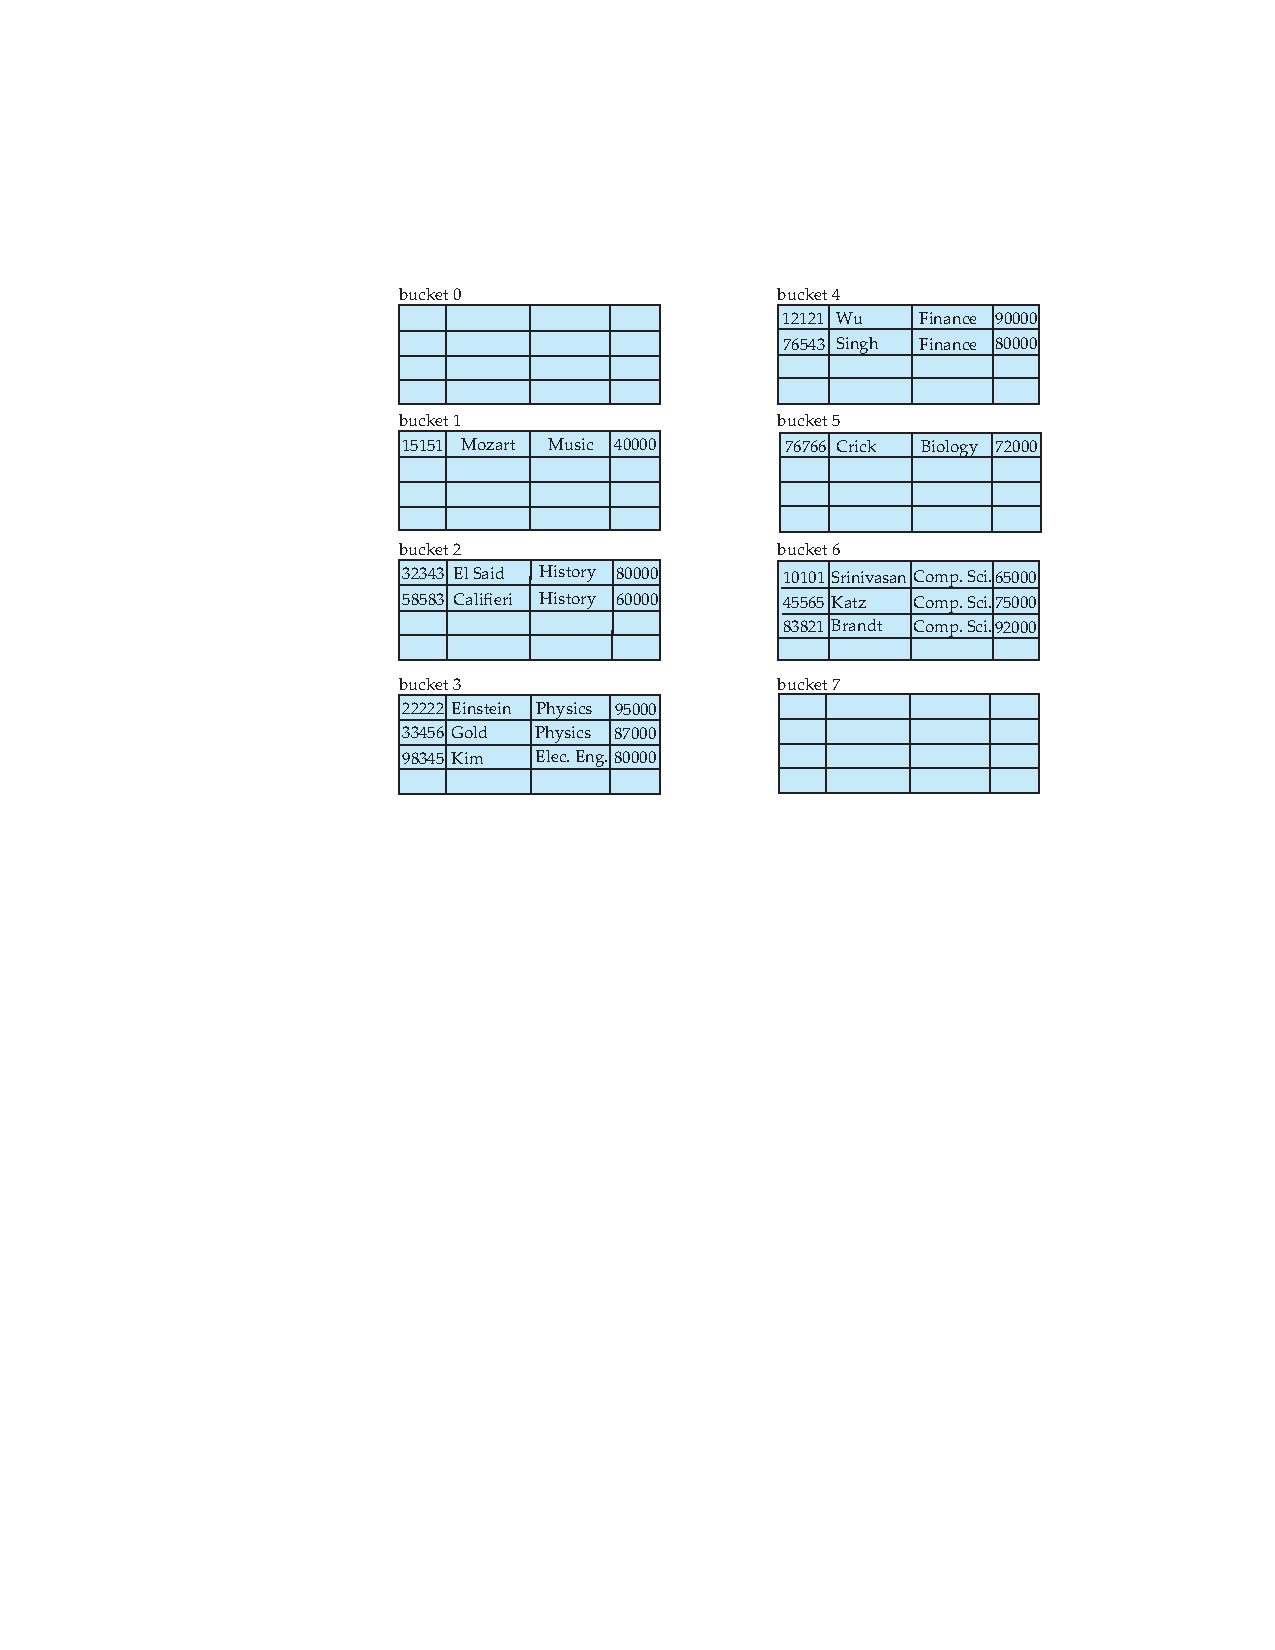
\includegraphics[width=0.6\textwidth]{aula06-hash1}
\caption{Organização de arquivo hash para \emph{instructor}, com
\emph{dept\_name} como chave de busca.}
\label{aula06:fig:hash1}
\end{figure}

\subsubsection{Funções hash}

A pior função mapeia todas as chaves de busca para o mesmo bucket, o que 
o tempo de acesso proporcional ao número de registros do arquivo.

Uma função ideal é \textbf{uniforme}: cada bucket recebe o mesmo número de chaves
de busca, a partir do conjunto de todos os valores possíveis.
Além disso, uma função ideal é \textbf{aleatória}: cada bucket recebe o mesmo número de 
chaves de busca, qualquer que seja a distribuição de chaves de busca real no
arquivo.

Funções típicas realizam o cálculo a partir da representação binária das chaves
de busca. 
Por exemplo, somando a representação binária dos caracteres e dividindo pelo número
de buckets.
O resto da divisão seria o bucket designado.

\subsubsection{Tratamento dos estouros de buckets}

Em caso de colisão, os registros que colidem ocupam o mesmo bucket e pode
ocorrer estouro do bucket (\emph{bucket overflow}).
O estouro pode ocorrer devido:
\begin{itemize}
\item buckets insuficientes.
\item Desequilíbrio na distribuição dos registros.
Os motivos são:
	\begin{itemize}
	\item muitos registros com a mesma chave de busca.
	\item a função de hash não é uniforme.
	\end{itemize}
\end{itemize}

Embora a probabilidade de estouro possa ser reduzida, ela não pode
ser eliminada.
Ela pode ser tratata através de \textbf{buckets de estouro}.
No \textbf{encadeamento de estouro}, os buckets de estouro são ligados
por uma lista encadeada (ver figura~\ref{aula06:fig:hash2}).
%
\begin{figure}[!htb]
\centering
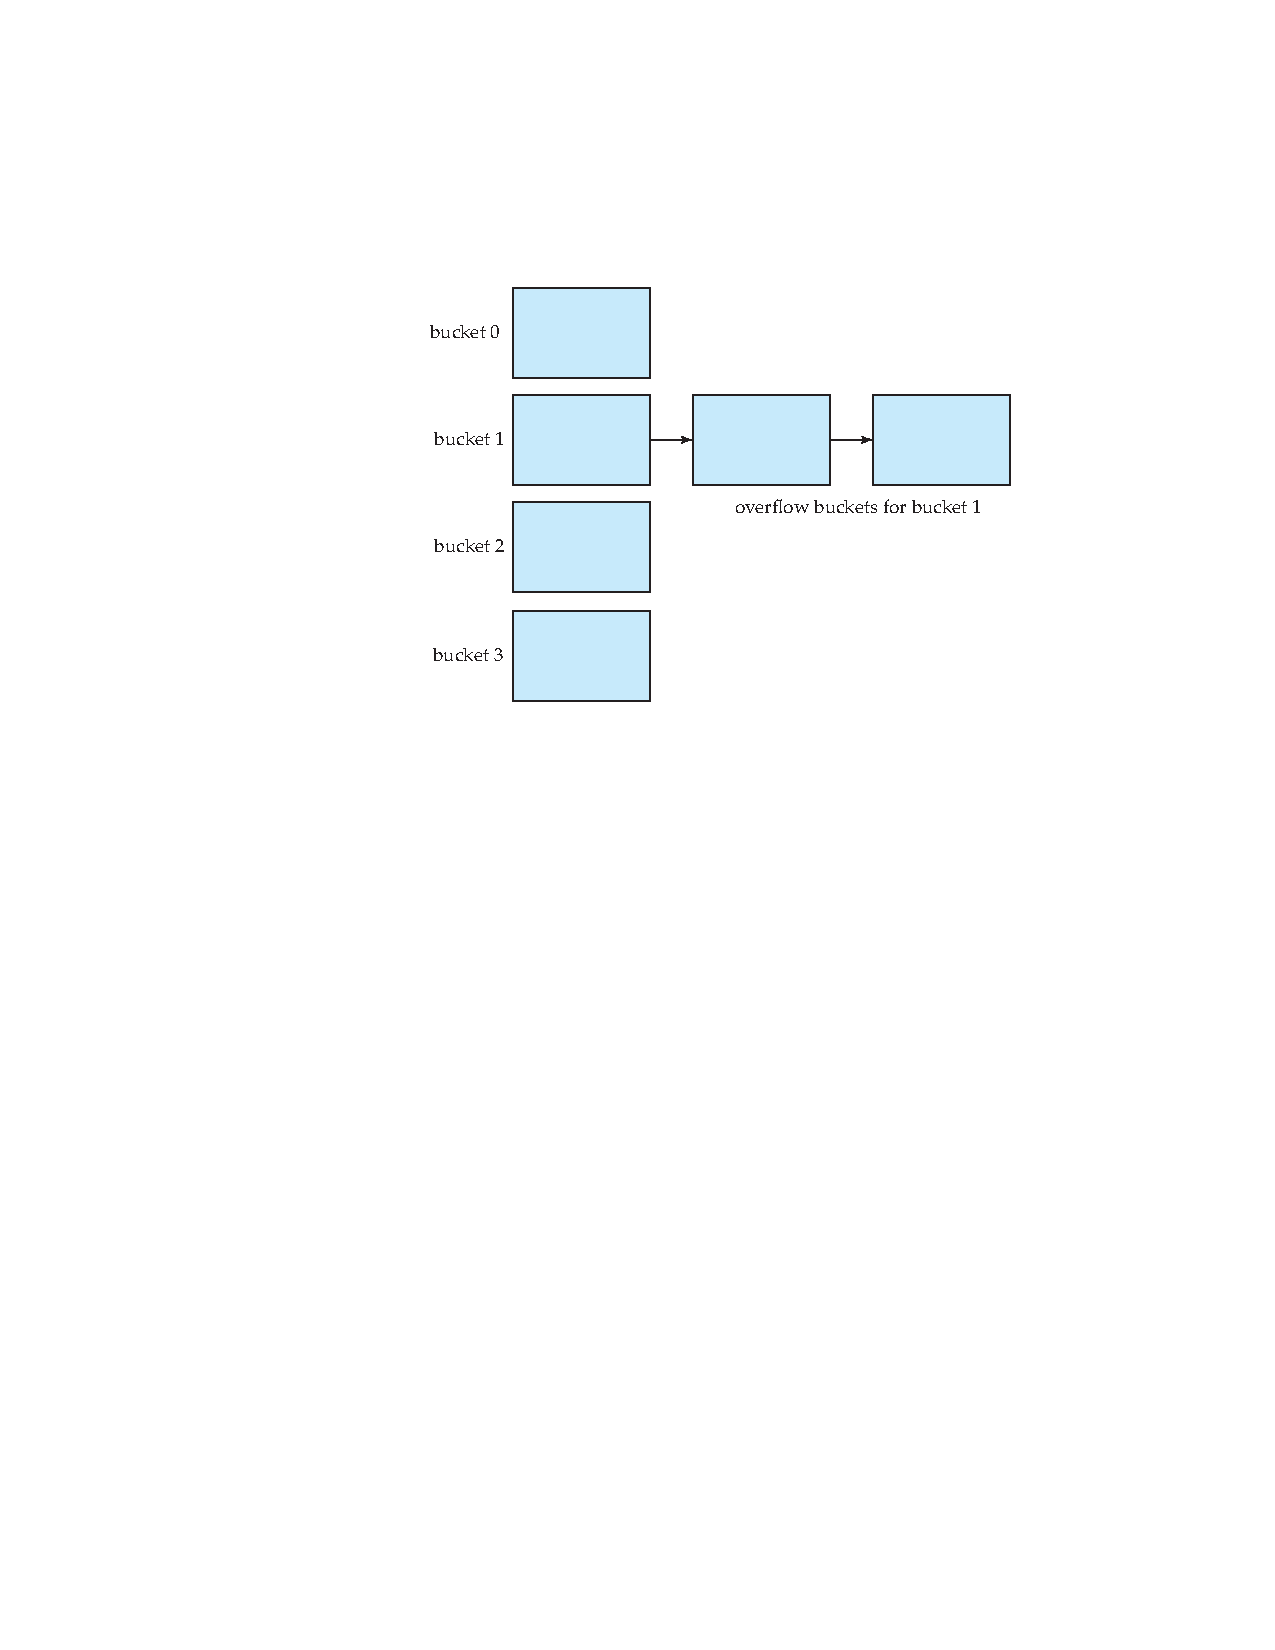
\includegraphics[width=0.5\textwidth]{aula06-hash2}
\caption{Exemplo de encadeamento de estouro.}
\label{aula06:fig:hash2}
\end{figure}

O esquema acima é chamado \textbf{closed hashing}. Uma outra alternativa,
chamada \textbf{open hashing}, não usa buckets de estouro.
Porém, não é adequada para aplicações de banco de dados.

\subsubsection{Índices hash}

Hashing também pode ser usado como índices. 
Um \textbf{índice hash} organiza as chaves de busca com seus ponteiros para registros.

\subsubsection{Deficiências do hashing estático}

No hashing estático, a função $h$ mapeia chaves de busca para um número fixo de buckets.
Com o crescimento ou encolhimento do banco de dados:
\begin{itemize}
\item Se o número de buckets for baixo, e o arquivo crescer, o desempenho
irá cair devido aos estouros.
\item Se o número de buckets for alto, uma grande quantidade de espaço
será desperdiçada inicialmente.
\item Se o arquivo encolher, novamente o espaço será desperdiçado.
\end{itemize}

Uma solução seria reorganização periódica do arquivo com uma nova função de hash.
Porém, essa solução custa caro e interrompe operações sobre o arquivo.
Uma solução melhor é permitir que o número de buckets seja modificado
dinamicamente.

%%%%%%%%%%%%%%%%%%%%%%%%%%%%%%%%%%%%%%%%%%%%%%%%%%%%%%%%%%%%%%%%%%%%%%%%%%%%%%%
\subsection{Hashing dinâmico}

Usado para bancos cujo tamanho costuma mudar, e permite que a função
de hash mude dinamicamente.
O \textbf{Hashing extensível} é uma das formas de hashing dinâmico.
A função de hash gera valores a partir de um intervalo elevado, tipicamente
inteiros com b-bits, onde $b = 32$.

Apenas um prefixo da função de hash é usado para indexar uma tabela de buckets.
Considere que a largura do prefixo seja de $i$ bits, $0 \leq i \leq 32$.
O tamanho da tabela de buckets é $2^i$, sendo inicialmente $i= 0$.
O valor $i$ cresce ou diminui junto com o banco de dados.

Múltiplas entradas da tabela de buckets podem apontar para o mesmo bucket. 
Assim, o número real de buckets é $< 2^i$. 
O número de buckets também muda dinamicamente pela sua mescla ou divisão.

Em uma hash extensível, cada bucket $j$ guarda o valor $i_j$. Todas as entradas
que apontam para o mesmo bucket tem o mesmo valor para os primeiros $i_j$ bits.
Para localizar o bucket contendo a chave de busca $k_j$:
\begin{enumerate}
\item Computar $h(K_j) = X$.
\item Usar os bits de maior ordem $i$ de $X$ como um deslocador na tabela
de buckets, e seguir o ponteiro para o bucket apropriado.
\end{enumerate}

\subsubsection{Inserção em estruturas de hash extensível}

Para inserir um registro com chave de busca $K_j$:
\begin{enumerate}
\item localizar o bucket apropriado $j$.
\item se tiver espaço no bucket $j$, inserir o registro no bucket.
\item senão, o bucket deve ser dividido e a inserção tentada de novo. 
Em alguns casos, são necessários buckets de estouro.
\end{enumerate}

Para dividir o bucket $j$ quando inserindo registro com a chave de busca $K_j$:
\begin{enumerate}
\item Se $i > i_j$ (mais de um apontador para o bucket $j$):
	\begin{enumerate}
	\item alocar um novo bucket $z$ e atribuir $i_j = i_z = (i_j+1)$.
	\item atualizar a segunda metade das entradas da tabela de 
	buckets que apontavam para $j$, fazendo-as apontar para $z$.
	\item remover os registros do bucket $j$ e reinseri-los 
	(em $j$ ou $z$).
	\item localizar o bucket para $K_j$ e inserir registro no bucket apropriado
	(realizar divisões sucessivas enquanto o bucket continuar cheio).
	\end{enumerate}

\item Se $i = i_j$ (apenas um ponteiro para o bucket $j$):
	\begin{enumerate}
	\item se $i$ atingir o limite $b$, ou se muitas divisões ocorrerem, criar um bucket
	de estouro.
	\item senão
		\begin{enumerate}
		\item incrementar $i$ e dobrar o tamanho da tabela de buckets.
		\item substituir cada entrada da tabela por duas entradas que
			apontam para o mesmo bucket.
		\item localizar a entrada na tabela de endereçamento para $K_j$.
		Agora $i > i_j$ estão no primeiro caso acima.
		\end{enumerate}
	\end{enumerate}

\end{enumerate}

A figura~\ref{aula06:fig:hash3} demostra a representação binária gerada pela função 
hash $h$ em uma chave de busca exemplo, enquanto que na figura~\ref{aula06:fig:hash4} ilustra
a estrutura do arquivo hash depois de 11 inserções.
%
\begin{figure}[!htb]
\centering
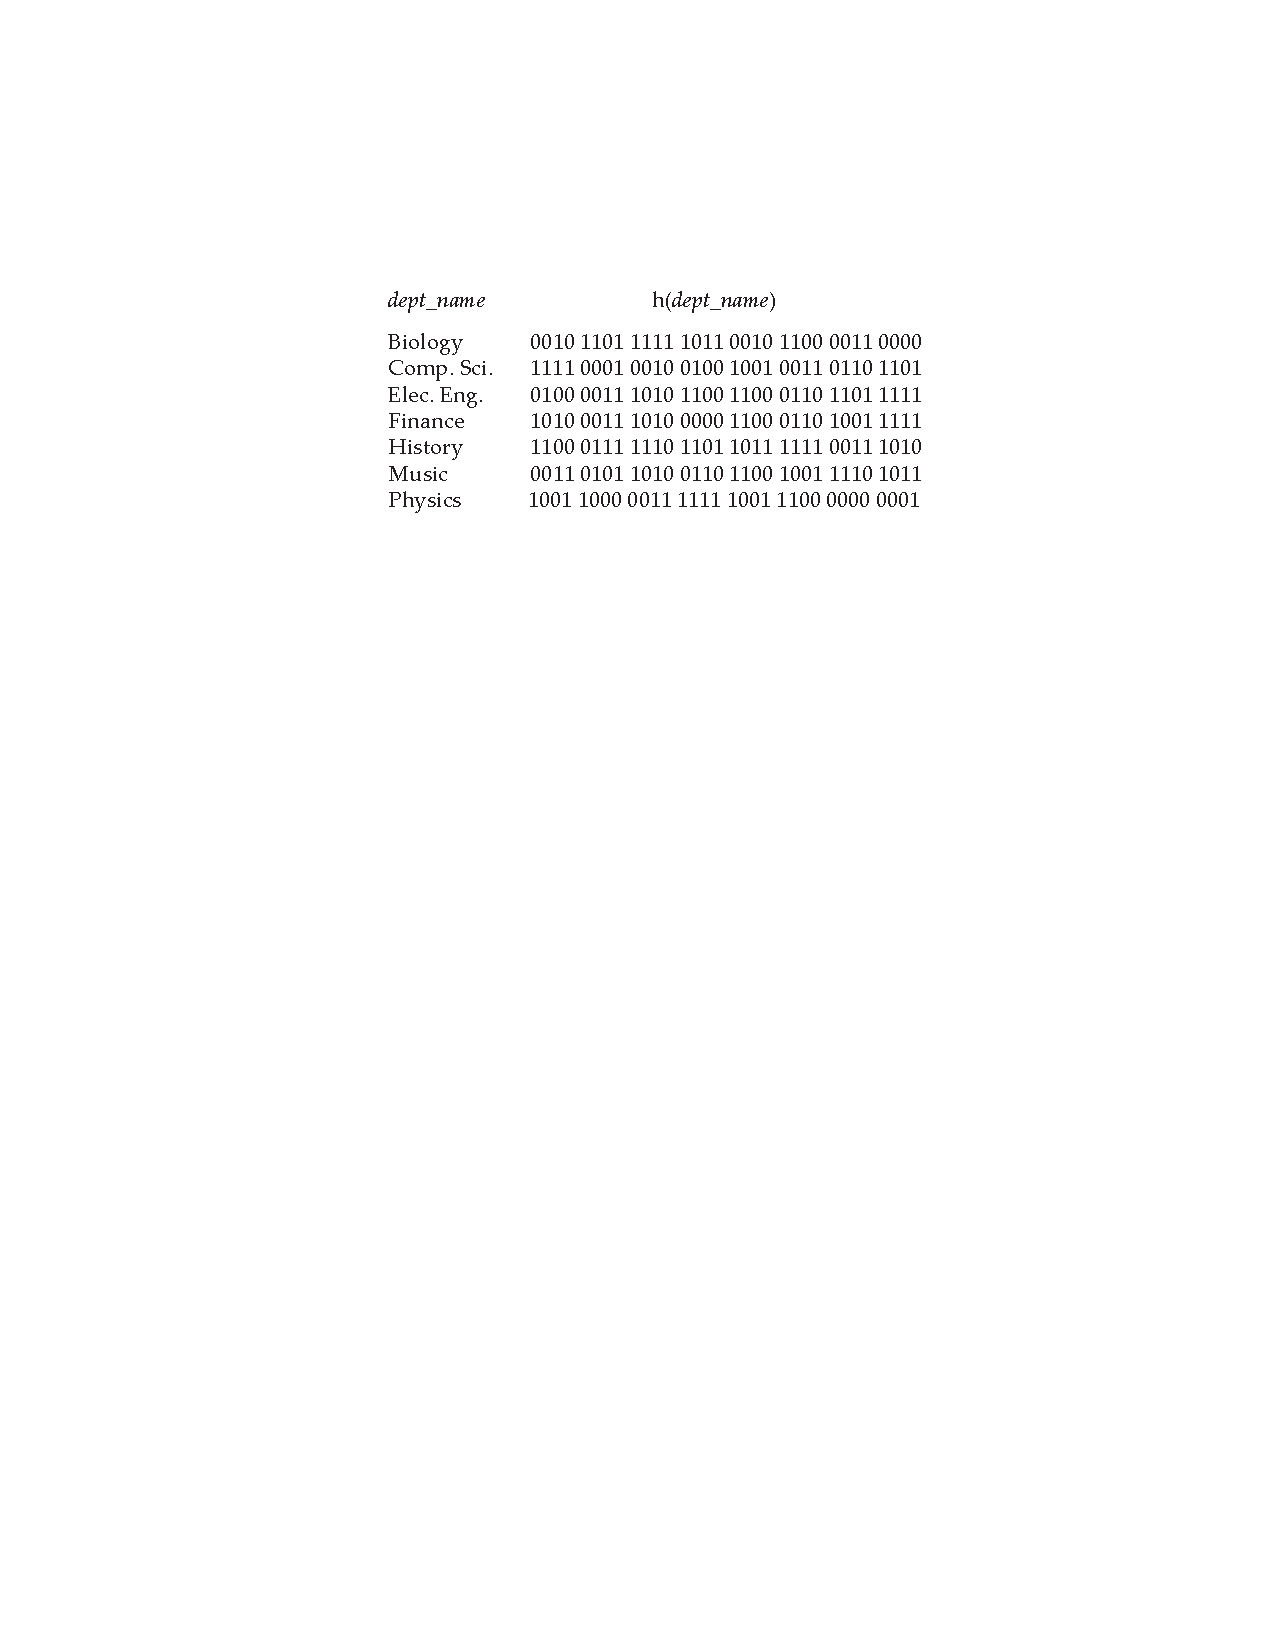
\includegraphics[width=0.6\textwidth]{aula06-hash3}
\caption{Função de hash extensível para o exemplo a seguir de inserção.}
\label{aula06:fig:hash3}
\end{figure}
%
\begin{figure}[!htb]
\centering
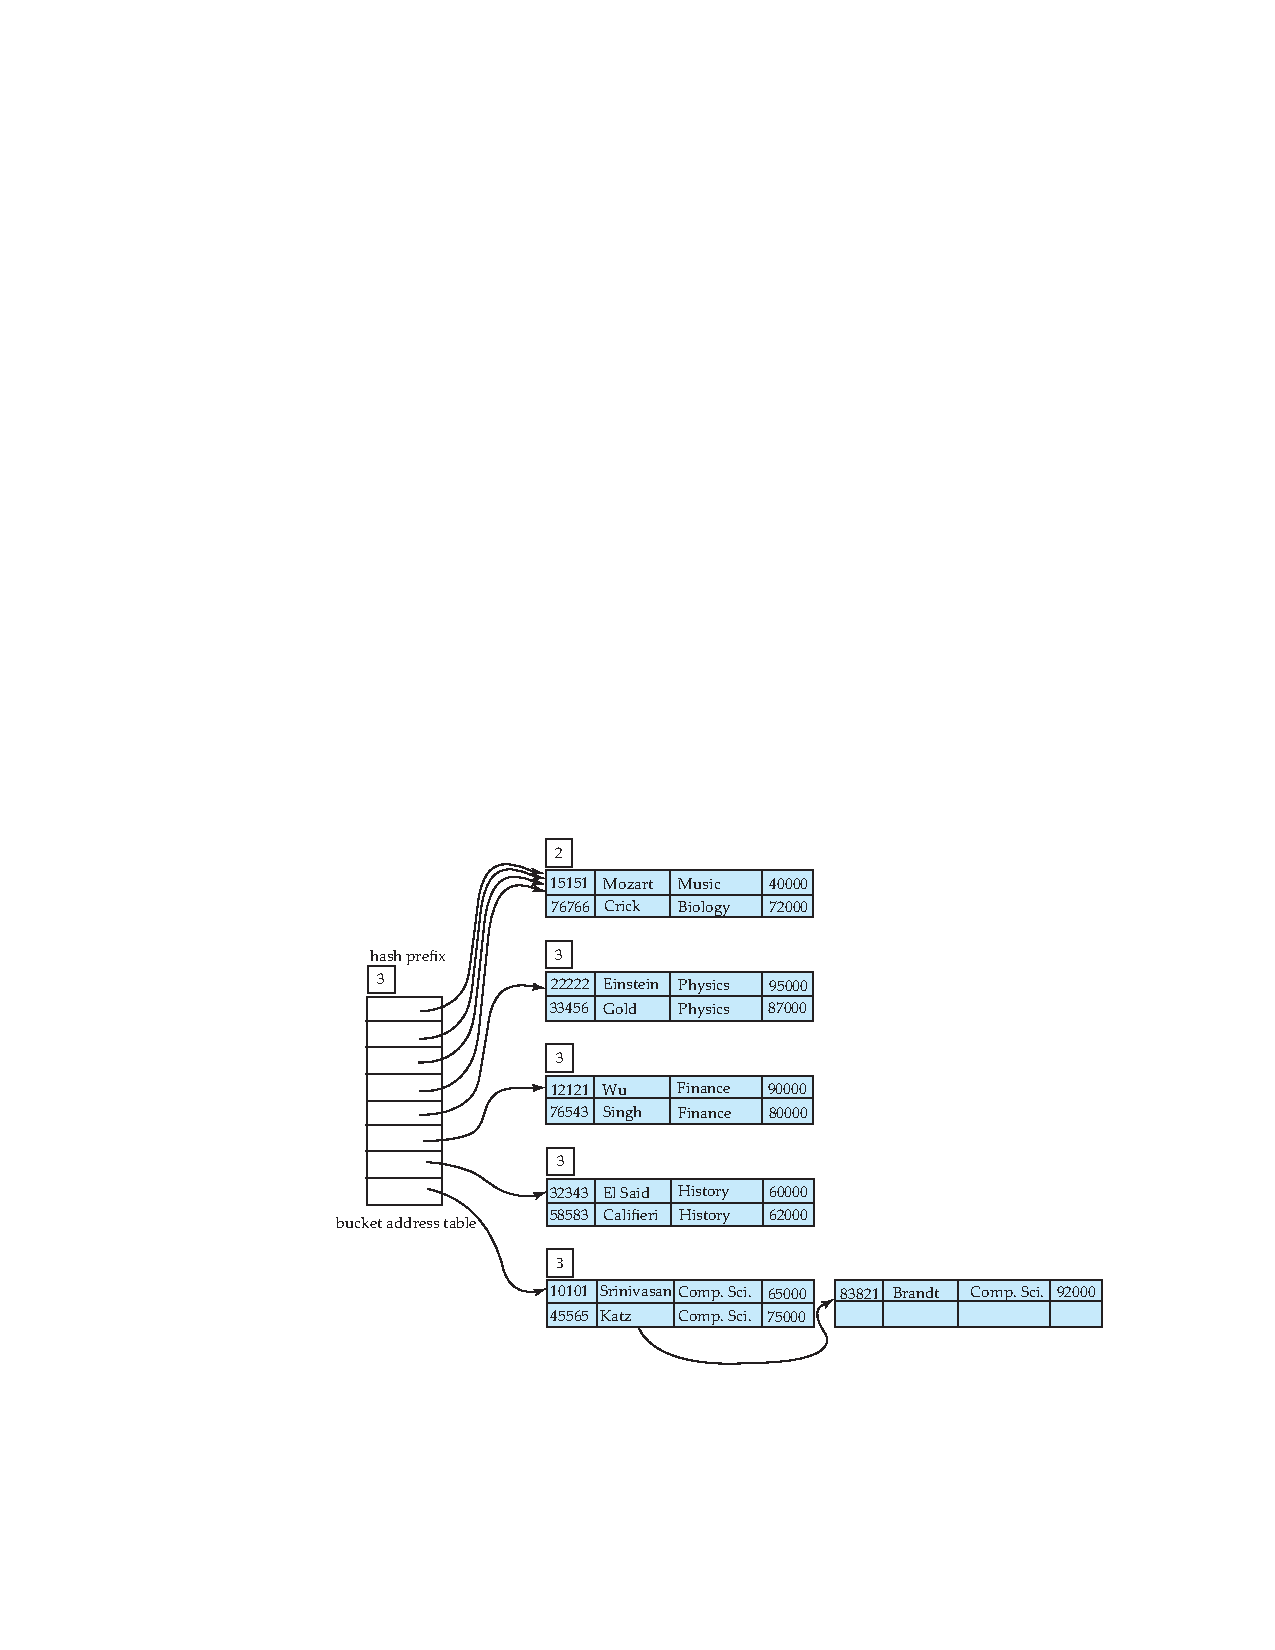
\includegraphics[width=0.7\textwidth]{aula06-hash4}
\caption{Estrutura do arquivo hash depois de 11 inserções.}
\label{aula06:fig:hash4}
\end{figure}


\subsubsection{Remoção em estruturas de hash extensível}

Para remover uma chave:
\begin{enumerate}
\item localizá-la no bucket e removê-la.
\item o bucket pode ser removido se ficar vazio (com as devidas
atualizações na tabela de buckets).
\item a mescla de buckets pode ser feita (pode mesclar apenas com
um bucket que tenha o mesmo valor $i_j$ e o mesmo prefixo $i_j-1$, se existir).
\end{enumerate}
A redução da tabela de buckets também é possível. Porém, a redução é cara
e deve ser feita apenas se o número de buckets for muito menor do que o tamanho
da tabela.

\subsubsection{Comparação com outros esquemas}

As vantagens do hash extensível são:
\begin{itemize}
\item O desempenho não degrada com o aumento do arquivo, sendo $C(n)=1$ se a 
função for uniforme e aleatória.
\item Sobrecarga de espaço é mínima.
\end{itemize}

As desvantagens são:
\begin{itemize}
\item Nível de indireção extra para localizar registros.
\item A tabela de buckets pode se tornar muito grande (maior que o espaço
disponível na memória).
	\begin{itemize}
	\item Não se pode alocar espaços contíguos em disco.
	\item Solução: usar uma árvore B+ para representar os registros em 
		uma tabela de buckets.
	\end{itemize}
\item Mudar o tamanho da tabela de endereço também é uma operação custosa.
\item Custo para recuperar os registros em ordem é alto.
\item Pior caso é $C(n) = n$.
\end{itemize}

%%%%%%%%%%%%%%%%%%%%%%%%%%%%%%%%%%%%%%%%%%%%%%%%%%%%%%%%%%%%%%%%%%%%%%%%%%%%%%%
\section{Índices compostos e bitmap}
%%%%%%%%%%%%%%%%%%%%%%%%%%%%%%%%%%%%%%%%%%%%%%%%%%%%%%%%%%%%%%%%%%%%%%%%%%%%%%%

\textbf{Chaves de busca compostas} são chaves de busca que possuem
mais de um atributo como em \emph{(branch\_name, balance)}.

\textbf{Índices de mapa de bits} (bitmap) foram projetados para responder com
eficiência consultas sobre mútiplas chaves.
Registros em uma relação devem possuir uma numeração sequencial. 
Dado um número $n$ deve ser fácil recuperar o registro $n$.

Um índice de bitmap é aplicável para atributos que assumem uma quantidade pequena de valores.
Exemplos são: sexo, país, estado, nível salarial (salário categorizado em níveis como 
0-9999, 10000-19999, 20000,50000, 50000-infinito).
Um mapa de bits é simplesmente um vetor de bits.

Um índice de bitmap sobre um atributo tem o um bitmap para cada valor possível
para esse atributo.
O bitmap tem tantos bits quantos forem os registros. 
Em um bitmap para o valor $v$, o bit para um registro é 1 se o 
registro possui o valor $v$, e 0 caso constrário.

Índices de bitmap são úteis para consultas por múltiplos atributos, e não muito úteis
para consultas por um único atributo.
Consultas são respondidas usando os seguintes operadores de bitmap:
\begin{itemize}
\item Interseção (\textbf{AND}).
\item União (\textbf{OR}).
\item Complementação (\textbf{NOT}).
\end{itemize}
Cada operação usa dois bitmaps de mesmo tamanho e aplica a operação nos bits
correspondentes para gerar o bitmap de resultado. Exemplos dessas operações são:
\begin{itemize}
\item Interseção -- 100110 \textbf{AND} 110011 = 100010
\item União --      100110 \textbf{OR} 110011 = 110111
\item Complementação -- \textbf{NOT} 100110 = 011001
\end{itemize}
Índices de bitmap geralmente são muito pequenos se comparados com o tamanho da tabela.

A figura~\ref{aula06:fig:bitmap1} mostra um exemplo de índice bitmap com a relação
de dois campos \emph{gender} e \emph{income\_level}. 
Por exemplo, em uma busca $gender = f(01101)$ e $income\_level = L2(01000)$ aplica-se a 
operação de interserção (AND) e resulta no bitmap $01000$.
%
\begin{figure}[!htb]
\centering
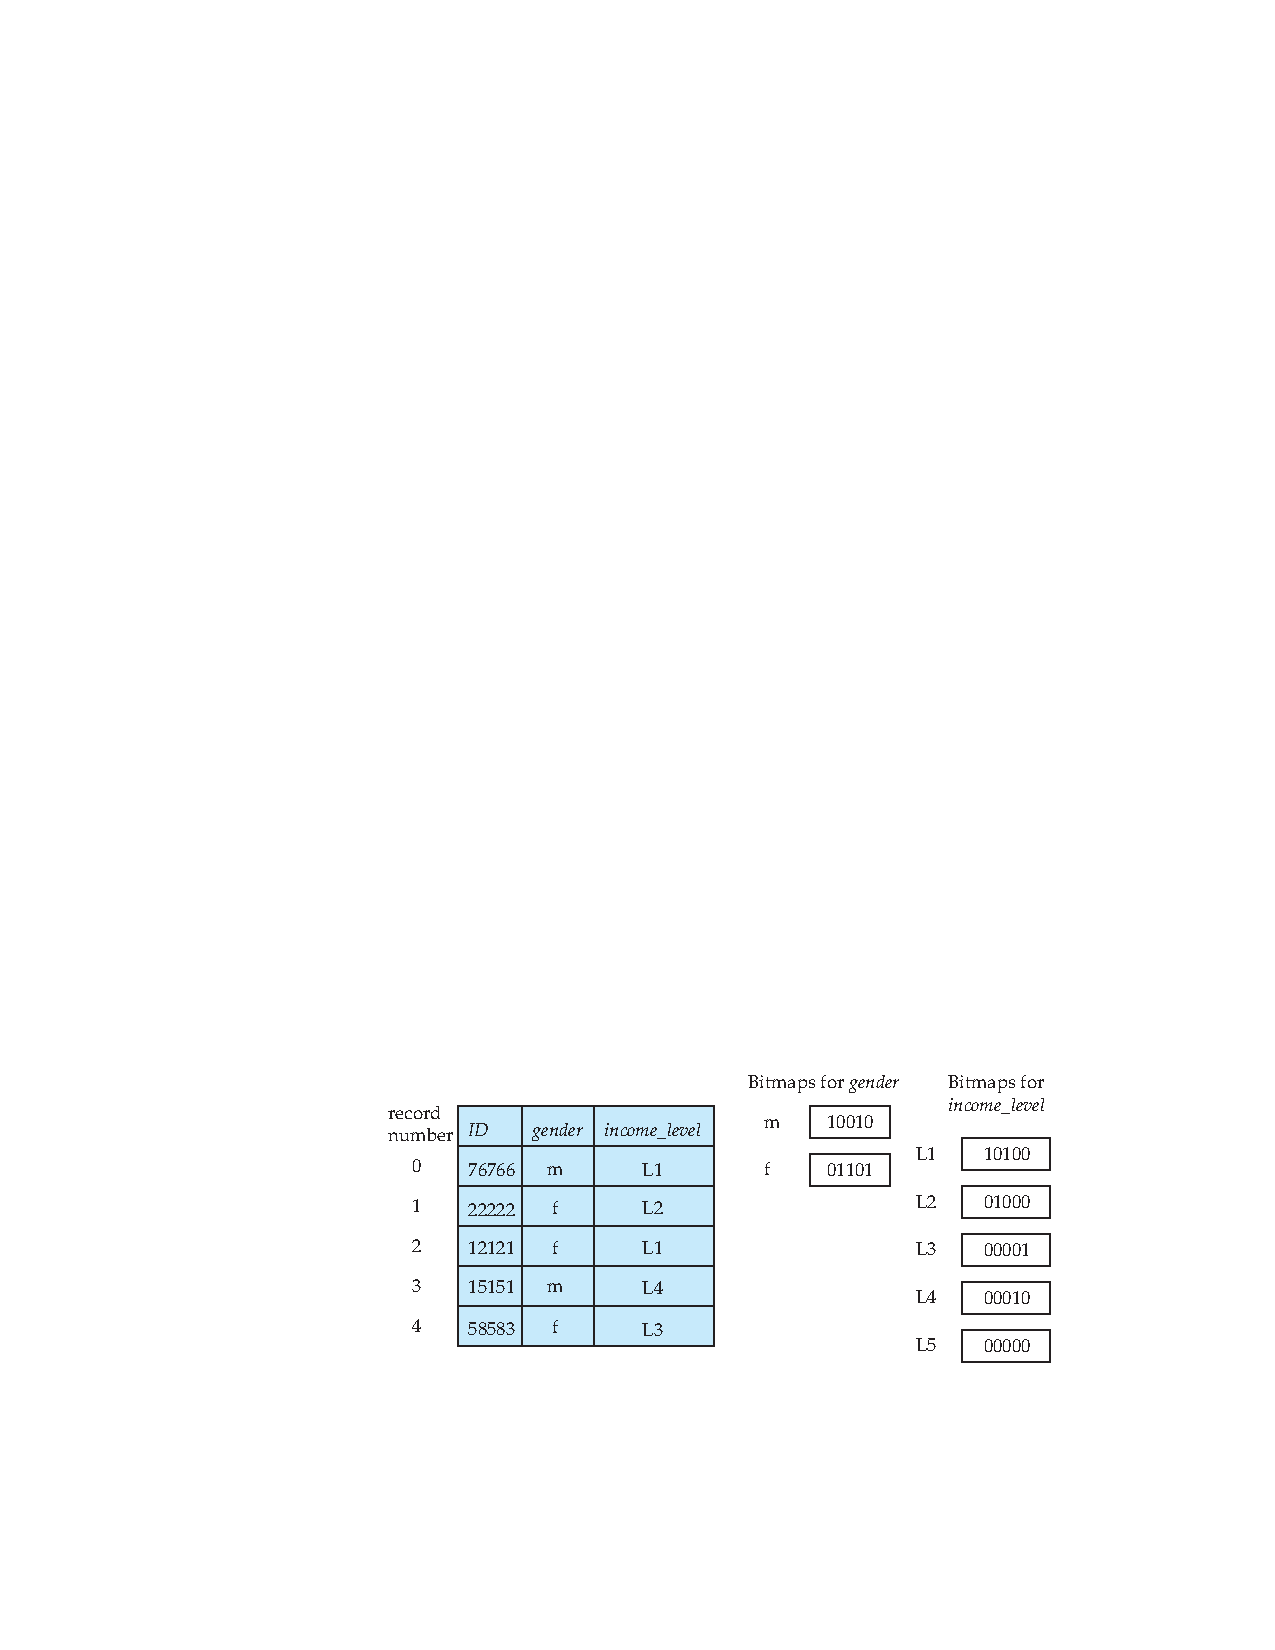
\includegraphics[width=0.6\textwidth]{aula06-bitmap1}
\caption{Índices bitmap para uma relação.}
\label{aula06:fig:bitmap1}
\end{figure}
%A operação de remoção precisa ser tratada de forma adequada.
%O \textbf{bitmap de existência} é necessário para operações de complementação,
%usada para averiguar se os registros ainda são válidos.

Quanto a implementação, bitmaps são empacotados em palavras, uma única palavra 
em uma instrução de CPU computa AND de 32 ou 64 bits de cada vez.
Por exemplo, um mapa com milhão de bits pode ser computado com apenas
31.250 instruções.

A contagem do número de 1s pode ser otimizada ao usar cada byte para indexar
um array de 256 posições.
Cada posição guarda a contagem de 1s na sua respectiva representação binária. 
Pode-se usar pares de bytes para agilizar o cálculo, com um custo
de memória adicional.
Em seguida, basta somar as contagens recuperadas.
Bitmaps podem ser usados nos nós folhas das árvores B+ em vez de listas 
de ponteiros de registros.
É vantajoso se $> 1/64$ dos registros tiver esse valor, supondo que o ponteiro
ocupe 64 bits.
Essa técnica combina vantagens dos bitmaps e das árvores B+.

%%%%%%%%%%%%%%%%%%%%%%%%%%%%%%%%%%%%%%%%%%%%%%%%%%%%%%%%%%%%%%%%%%%%%%%%%%%%%%%
\section{Índices multidimensionais}
%%%%%%%%%%%%%%%%%%%%%%%%%%%%%%%%%%%%%%%%%%%%%%%%%%%%%%%%%%%%%%%%%%%%%%%%%%%%%%%

Os atributos usados em uma busca podem ser considerados como dimensões.
Consultas que envolvem buscas em mais de um atributo ou dimensão podem
usar dois tipo de índices.
\begin{itemize}
\item Índices unidimensionais.
\item Índices multidimensionais.
\end{itemize}

Em índices unidimensionais a chave de pesquisa é única. Também é possível
recuperar registros que correspondem a um dado valor (ou intervalo)
da chave de busca. Os tipos de índices podem ser:
\begin{itemize}
\item Índices ordenados - arquivos sequenciais e árvores B+.
\item Tabelas hash.
\end{itemize}

\textbf{Índices multidimensionais} são usados para consultas em mais do que um atributo
(ou dimensão).
A estruturas de índices multidimensionais podem ser baseadas em:
\begin{description}
\item[Tabelas hash] a resposta da consulta pode não estar em um único bucket. Contudo,
pode estar em um número baixo de buckets.

\item[Árvores] não há correspondência entre os nós da árvore e blocos do disco.
Todavia, árvores podem ficar desbalanceadas e a eficiência nas atualizações pode ser menor.

\end{description}

%%%%%%%%%%%%%%%%%%%%%%%%%%%%%%%%%%%%%%%%%%%%%%%%%%%%%%%%%%%%%%%%%%%%%%%%%%%%%%%
\subsection{Arquivos de grade}

%%%%%%%%%%%%%%%%%%%%%%%%%%%%%%%%%%%%%%%%%%%%%%%%%%%%%%%%%%%%%%%%%%%%%%%%%%%%%%%
\subsection{Funções de hash particionado}

%%%%%%%%%%%%%%%%%%%%%%%%%%%%%%%%%%%%%%%%%%%%%%%%%%%%%%%%%%%%%%%%%%%%%%%%%%%%%%%
\subsection{Índices de várias chaves}

%%%%%%%%%%%%%%%%%%%%%%%%%%%%%%%%%%%%%%%%%%%%%%%%%%%%%%%%%%%%%%%%%%%%%%%%%%%%%%%
\subsection{Árvores kd}

%%%%%%%%%%%%%%%%%%%%%%%%%%%%%%%%%%%%%%%%%%%%%%%%%%%%%%%%%%%%%%%%%%%%%%%%%%%%%%%
\subsection{Árvores de quadrante}

%%%%%%%%%%%%%%%%%%%%%%%%%%%%%%%%%%%%%%%%%%%%%%%%%%%%%%%%%%%%%%%%%%%%%%%%%%%%%%%
\subsection{Árvores R}

%%%%%%%%%%%%%%%%%%%%%%%%%%%%%%%%%%%%%%%%%%%%%%%%%%%%%%%%%%%%%%%%%%%%%%%%%%%%%%%
\section{Exercícios}
%%%%%%%%%%%%%%%%%%%%%%%%%%%%%%%%%%%%%%%%%%%%%%%%%%%%%%%%%%%%%%%%%%%%%%%%%%%%%%%



\end{document}
